\documentclass[12pt]{article}
\usepackage[utf8]{inputenc}
\usepackage{multibbl}
\usepackage{hyperref}
\newbibliography{article}
\newbibliography{SI}

% Usage of multibbl:
% bibtex artile
% bibtex SI

%\usepackage[sectionbib,numbers]{natbib}
\usepackage{eurosym}
\usepackage{float}
\usepackage{amstext,amsthm}
\usepackage{amsmath}
\usepackage{amssymb,mathtools}
\usepackage[nointegrals]{wasysym} % enthaelt iint-Def die aber auch in amsmath definiert sind
\usepackage{mathrsfs}
% \usepackage{refcheck}
\usepackage{graphicx}
\usepackage[figuresleft]{rotating}
\usepackage{rotating, float, caption}


\usepackage{tikz,color,a4wide,tabularx}
\usetikzlibrary{shapes.geometric}
%\usepackage{enumerate}

\newtheorem{proposition}{Proposition}[section]
\newtheorem{corollary}[proposition]{Corollary}
\newtheorem{theorem}{Theorem}
\newtheorem{lemma}{Lemma}[section]
\theoremstyle{definition}
\newtheorem{definition}{Definition}[section]
\newtheorem{remark}{Remark}[section]
\newtheorem{example}{Example}[section]
\newtheorem{estimator}{Estimator}[section]
\pagestyle{headings}

% \setlength{\bibsep}{0pt}

\setlength{\textheight}{230mm}
\setlength{\topmargin}{-15mm} 
\setlength{\textwidth}{17cm} 
\setlength{\oddsidemargin}{-3mm}
\setlength{\columnseprule}{.1pt}
\setlength{\columnsep}{20pt}

\def\blstr{1.1}
\renewcommand{\baselinestretch}{\blstr}
\def\blstrtable{1.55}
\def\blstrcode{1.2}  
%\renewcommand{\labelenumi}{\alph{enumi})}
%%\setlength{\oddsidemargin}{0.28in} 
%%\setlength{\evensidemargin}{0.28in}

%\addtolength{\bibsep}{1.5mm}
%%\bibpunct{(}{)}{,}{a}{}{,}

%%\RequirePackage{ae,mathpple}
%%\renewcommand{\rmdefault}{ppl}
%%\renewcommand{\sfdefault}{aess}
%%\renewcommand{\ttdefault}{aett}
\newcommand{\Rpackage}[1]{{\normalfont\fontseries{b}\selectfont #1}}

%\usepackage{a4}
\usepackage[normalem]{ulem}
\usepackage{color}
\newcommand\crule[3][black]{\textcolor{#1}{\rule{#2}{#3}}}

\newcommand{\dirk}[3]{\textcolor{red}{\sout{#1}\textcolor{blue}{#2}}{\begin{marginpar}{\raggedright\color{red} Dirk:\tiny {#3}}\end{marginpar}}}
\newcommand{\peter}[3]{\textcolor{red}{\sout{#1}\textcolor{blue}{#2}}{\begin{marginpar}{\raggedright\color{green} Peter:\tiny {#3}}\end{marginpar}}}


\DeclareMathAlphabet{\mathpzc}{OT1}{pzc}{m}{it}
\newcommand{\smallu}{\mathpzc{u}}
\newcommand{\smallx}{\mathpzc{x}}
\newcommand{\smally}{\mathpzc{y}}
\newcommand{\smallz}{\mathpzc{z}}
\newcommand{\ind}[1]{\mathbbm{1}_{\{#1\}}} %Definition Indikatorfunktion
\newcommand{\indset}[1]{\mathbbm{1}_{#1}} %Definition Indikatorfunktion
\providecommand{\abs}[1]{\lvert#1\rvert}
\providecommand{\norm}[1]{\lVert#1\rVert}

\usepackage{xcolor}
\definecolor{colAMR}{RGB}{255,0,0}
\definecolor{colAFR}{RGB}{255,191,0}
\definecolor{colEUR}{RGB}{128,255,0}
\definecolor{colEAS}{RGB}{255,0,191}
\definecolor{colSAS}{RGB}{0,255,255}
\definecolor{colMEA}{RGB}{0,64,255}
\definecolor{colOCE}{RGB}{128,0,255}
\definecolor{colSIB}{RGB}{0,255,64}



\usepackage{times}
%%\RequirePackage[T1]{fontenc}

\begin{document}
\title{\LARGE Inference of recent admixture using genotype data}

\author{\sc Peter Pfaffelhuber, Elisabeth Huss, Franz Baumdicker, \\
  \sc Jana Naue, Sabine Lutz-Bonengel, Fabian Staubach}

\date{\today}

\maketitle

\begin{abstract}
  \noindent
  For inference of individual genetic histories, admixture barplots
  are being used abundantly in forensic genetics. These plots
  visualize parameters for individual ancestry (IA), as inferred from
  the admixture-model, as e.g.\ implemented in the software {\sc
    structure} and {\sc admixture}. In this model, it is assumed that
  every allele in the individual's genome originates in one of several
  ancestral populations with the same probability. We will showcase
  that estimates of IA might be inaccurate in cases of recent
  adxmixture. As a way out, we introduce the recent-admixture model,
  which makes use of the excess of heterozygotes observed in recently
  admixed individuals. In this model, we assume that the two
  homologous copies of each allele originate from the ancestral
  populations independently for the mother's and the father's
  copy. Estimates for IA in absence of recent admixture are almost
  identical for the admixture and recent admixture model. However,
  they are more accurate for the recent-admixture model in individuals
  which are in fact recently admixed. Moreover, we develop a
  likelihood ratio test for recent admixture, which has a high power
  to find recently admixed individuals. We analyse data from the 1000
  genomes dataset with our methods and find some recently admixed
  individuals.
\end{abstract}

\section{Introduction}
Inference of the geographical ancestry of a trace using genetic
markers is today a well-established research field in forensic
genetics (see e.g.\ \cite{article}{Phillips2016, Eduardoff2016,
  Kidd2017}). Either the trace is classified into one of several
groups of different origin (e.g.\ Africa, Europe, East Asia, Native
America, and Oceania; see e.g.\ \cite{article}{Snipper2007,
  Pfaffelhuber2019}, or it is assumed that it consists of a mixture of
ancestral genetic material originating in several groups. For this
task, {\sc structure} \cite{article}{Pritchard2000} has become the
de-facto standard to estimate individual ancestry (IA) proportions of
a trace among several continental groups. This Bayesian approach using
MCMC was complemented by the faster, likelihood based approach,
implemented in the software {\sc admixture}
\cite{article}{Alexander2009}; see also \cite{article}{Tang2005} for
the same model.

When using {\sc structure} or {\sc admixture} for estimating
continental (or other scales of geography) IA of a trace, allelic
frequencies for all continents from a reference database must be
used. A main assumption for estimating IAs is that all allelic states
have the same independent chance to share a copy from some continent.
When using a (small) set of ancestry informative markers, the large
genomic distance makes loci almost independent by recombination,
resulting in independence of markers across loci. However,
independence of the two copies at the same marker, usually denoted by
Hardy-Weinberg equilibrium, may not always hold. For example, consider
an individual whose parents have different continental backgrounds,
$A$ and $B$, say, and an allele which separates perfectly between the
two continents. Then, the individual will certainly be a heterozygote
at this marker. This increase in frequency for heterozygotes under
admixture is known for a long time and usually called the Wahlund
effect \cite{article}{Wahlund1928}.  However, {\sc structure} and {\sc
  admixture} will estimate that the chance for some allele to come
from $A$ and $B$ to be 50\%, which is then also be the estimated
probability for a heterozygote at the locus (due to the assumption of
independence of allelic states in the admixture model).

In general, {\sc structure} (and {\sc admixture}) are able to give
accurate estimates of IA also in the case of recent-admixture. As
observed in \cite{article}{Cheung2018}, {\sc structure} outperforms a
newly developed Genetic Distance Algorithm preforms in almost all
cases of recent admixture (except for the case when all four
grand-parents come from different populations). However, {\sc
  structure} does not reveal all relevant information in the data in
the case of recent admixture, since e.g.\ an IA of 50\% $A$ and 50\%
$B$ either indicates two parents with these IAs or a recent admixture
event of one individual from $A$ and one from $B$.

Our goal is to be able to distinguish these cases by making use of the
Wahlund effect, which will also result in better estimates of IA. So,
we aim for (i) improving estimates of IA and (ii) detecting recent
admixture. In particular, we extend the likelihood-model behind {\sc
  structure} or {\sc admixture} in order to account for recent
admixture. In the resulting recent-admixture-model, IA consists of two
vectors, one for each parent. We will call this pair of vectors
Parental Individual Admixture, PIA. So, in the above example, the
recent-admixture-model would estimate father and mother to have IAs as
100\% $A$ and 100\% $B$, respectively, due to the excess of
heterozygotes.  Since we are using only autosomal markers, we cannot
distinguish which of the parents comes from $A$ and $B$, though. Then,
with the estimate of PIA, the estimated probability for a heterozygote
is~1 in the example. Let us mention that in some occasions, {\sc
  STRUCTURE} draws wrong conclusions on DNA of recently admixed
individuals. We see in simulations, that a recently admixed from two
distant populations is estimated to come mainly from some intermediate
location.

The excess of heterozygotes was recently used to detect recent
admixture using statistical tests. For example,
\cite{article}{McNevin2019} uses a statistical test by simply counting
the number of heterozygous positions in an individual in order to
infer recent admixture. A different approach is used by
\cite{article}{Tvedebrink2018, Tvedebrink2019}. Here,
likelihood-ratio tests were developed which test the null-hypothesis
of non-admixture and recent (first generation) admixture versus the
alternative that the studied sample is not represented in the
reference database. We complement this test by observing that the
adxmixture model is a special case of the recent-admixture model, if
the IA of both parents is the same. This paves the way to give a
likelihood-ratio-test for recent admixture, with equality of the
parental IAs as null-hypothesis. The alternative hypothesis, however,
is that the studied sample shows recent admixture of populations
within the reference database.

As exemplary cases, we present data from two (one female and one male)
individuals whose DNA was collected during a study in Freiburg,
Germany. The female individual self-reported to have a father from
Germany and a mother from the Philippines. Her mtDNA haplotype based
on the control region sequencing was found three times so far in the
EMPOP database (out of 38361 samples) with two matches on the
Philippines and belongs to the haplogroup F1a4a1. This stands in
accordance with the self-reported ancestry of the maternal
lineage. The male individual self-reported to have a father from Italy
and a mother from Venezuela. His mtDNA haplotype was not yet observed
(no exact match), but belongs to the haplogroup A2+64 which is mostly
found in Central America. No samples with that haplogroup were seen in
Venezuela yet. However, only 101 reference samples are available in
EMPOP covering Native American in Venezuela. The minimal Y-chromosomal
haplotype was observed worldwide another times within the YHRD
database with four occurrences in Italy. For both samples, the
recent-admixture model correctly picks up the different origins of the
genetic material from 53 aurosomal SNPs, but only in one case places
the ancestors in proximity to the reported ones.

% As showcases, we present data from a (female) individual whose DNA was
% collected during a study in Freiburg, Germany, and analyse the 1000
% genomes dataset for recent admixture. For the former, the individual
% self-reported to have a father from Germany and a mother from the
% Philippines. Here, when using a classification tool such as {\sc
%   Snipper} \cite{article}{Snipper2007}, her DNA is classified as
% South-East-Asian (i.e.\ close to reference samples from India,
% Pakistan etc). The ForenSeq Universal Analysis Software did not
% provide a clear classification result into one cluster, but states the
% closest centroid in which also samples from the 1000 genomes
% populations mainly from Puerto Rico and Colombia fall into. While the
% admixture model correctly estimates ancestral proportions from Europe,
% East-Asia and Oceania, the recent-admixture model clearly identifies a
% recently admixed genome. In addition, the mt-DNA of her and therefore
% the maternal lineage belongs to the haplogroup F1a4a1 which was
% observed on the Philippines and in Japan using the EMPOP database and
% stands in accordance with the self-reported ancestry of the mother.
% For the latter, the analysis of the 1000 genomes dataset, we detect
% individuals with a high chance of recent admixture from Africa
% (population ASW, African Americans) and a moderate chance of recent
% admixture from South Asia (BEB, Bangli and GIH, Gujarati Indian from
% Houston).

\section{Materials and Methods}
We start by briefly recalling the admixture model, which is the basis
for the widely used sofware {\sc structure} \cite{article}{Pritchard2000}, {\sc
  admixture} \cite{article}{Alexander2009} and {\sc frappe} \cite{article}{Tang2005}.
Afterwards, we introduce a new model, called the recent-admixture
model. More details on the derivations in the admixture and
recent-admiture model can be found in the SI. Moreover, the
implementation of our methods can be downloaded from \url{
  https://github.com/pfaffelh/recent-admixture}. For both, the
adxmiture and recent-admixture model, we assume to have reference
database of $M$ bi-allelic markers from $K$ populations. However, from
this reference database, we only need to known allele frequencies,
i.e.\ by $p_{mk}$, the frequency of allele~1 at marker $m$ in
population $k$ for all $m=1,...,M$ and $k=1,...,K$. We have a trace
with $G_m \in \{0,1,2\}$ copies of allele~1 at marker $m$ for
$m=1,...,M$.  We will assume throughout that the allele frequencies
$p_{mk}$ are given and will not be changed by analysing the
trace. This is important since in currently used software {\sc
  structure}, {\sc admixuture} and {\sc frappe}, mostly in
non-forensic use, it is frequently the case that many new individuals
are studied, and allele frequencies are updated. For forensic use,
when analysing several traces at once, this would imply that the
results for the ancestry of trace~1 depend not only on the reference
data, but also on the data for traces~2, 3,... which seems
inappropriate. Hence, we do not make the computational overload of
updating allele frequencies, which would also lead to increased
runtimes and take the allele frequencies as given in the reference
database. With other words, we will follow the approach of
\cite{article}{Chakraborty1986} and \cite{article}{Hanis1986} for analysing our models.

\subsection{The admixture model}
Assuming that each allele observed in the trace comes from population
$k$ with probability $q_k$, the probability to observe allele~1 at
marker $m$ is
\begin{align}
  \label{eq:beta}
  \beta_m(q) := \sum_k p_{mk} q_k,  
\end{align}
and the log-likelihood of $q = (q_k)_{k=1,...,K}$ is (see
also~\eqref{Seq:lik} in the SI)
\begin{align}\label{eq:logLadmixture}
  \ell(q|G) = \sum_{m=1}^M \log\Big(\binom{2}{G_m} \beta_m(q)^{G_m}(1-\beta_m(q))^{2-G_m}\Big).
\end{align}
Assuming that all $p_{mk}$'s are known, this function can be maximized
over $q$ by computing $\hat q = (\hat q_k)_{k=1,...,K}$ such that
$\hat q_k = f_k(\hat q)$ for (see also \eqref{eqSI:fixed} in the SI)
\begin{align}\label{eq:fixed}
  f_k(q) =
  \frac{1}{2M} \sum_{m=1}^M \Big(G_m \frac{p_{mk}}{\beta_m(q)} + (2-G_m)\frac{1-p_{mk}}{1-\beta_m(q)}\Big)q_k,
  \qquad k =1,...,K.
\end{align}
This can be done numerically by iterating
$q_{n+1} = (f_k(q_n))_{k=1,...,K}$ until convergence. (In our
implementation, we continue the iteration until
$|q_{n+1} - q_n|< 10^{-6}$.) We note that this approach is essentially
the same as in the EM-algorithm from \cite{article}{Tang2005}, but
combining the expectation and maximization steps, since we do not
update allele frequencies. In addition, although maximizing
\eqref{eq:logLadmixture} could also be handled using a Newton method
as in \cite{article}{Alexander2009}, this approach has the advantage
that $q_n$'s are positive in all steps, and the sum of all entries in
$q_n$ is always~1. Moreover, the iteration is computationally fast if
only a small or moderate number of alleles is considered.

\subsection{The recent-admixture model}
When mother and father of an individual come with their own vectors of
admixture proportions, $q^M$ and $q^P$, the log-likelihood from
\eqref{eq:logLadmixture} changes to (see also
\eqref{eqSI:logLrecentadmixture} in the SI)
\begin{align}\label{eq:logLrecentadmixture}
  \ell(q^M, q^P|G) & = \sum_{m=1}^M \log( \gamma_m(q^M, q^P, G_m)),
  \\
  \notag
  \gamma_m(q^M, q^P, g) & = \begin{cases}\beta_m(q^M) \beta_m(q^P), & \text{ if }g=2,\\
    (\beta_m(q^M) (1-\beta_m(q^P))
    + (1-\beta_m(q^M)) \beta_m(q^P)), & \text{ if }g=1,\\
    (1-\beta_m(q^M))(1-\beta_m(q^P)), & \text{ if }g=0. \end{cases}
\end{align}
\sloppy As carried out in the SI, this function can be maximized by
computing $\hat q^M, \hat q^P$ such that
$\hat q^P = f(\hat q^M, \hat q^P)$ and
$\hat q^M = f(\hat q^P, \hat q^M)$ for
$f(q,q') = (f_k(q, q'))_{k=1,...,K}$ with (see
\eqref{eqSI:fixedRecent} in the SI)
\begin{align}\label{eq:fixedRecent}
  f_k(q, q') & := \frac{1}{M}\sum_{m=1}^M \delta_k(q,q', G_m) q_k',
  \\
  \notag
  \delta_k(q^M, q^P, g) & = \begin{cases}
    \displaystyle\frac{p_{mk}}{\beta_m(q')}, & \text{ if }g=2,\\[2ex]
    \displaystyle\frac{(p_{mk} (1-\beta_m(q))
      + (1-p_{mk})\beta_m(q))}{\beta_m(q)(1-\beta_m(q'))
      + (1-\beta_m(q))\beta_m(q')}, & \text{ if }g=1,\\[2ex]
    \displaystyle\frac{(1-p_{mk})}{1-\beta_m(q')}, & \text{ if }g=0. \end{cases}
\end{align}
In our implementation, we iteratively compute
$q_{n+1}^P = f(q_n^M, q_n^P)$ and $q_{n+1}^M = f(q_{n+1}^P, q_n^M)$
until convergence.

\subsection{Obtaining admixed individuals in silico}
\label{S:insilico}
In order to test our method, we created admixed individuals from a
reference database. (We use the 1000 genomes dataset, but excluding
Admixed Americans, AMR; see below.) For example, we obtain an
individual admixed from populations $k$ and $k'$ by choosing a genome
$\tilde G = (\tilde G_m)_{m=1,...,M}$ from population $k$ and
$\bar G = (\bar G_m)_{m=1,...,M}$ from population $k'$ as the
parents. Then, $(G_m)_{m=1,...,M}$ are independent with
$G_m = X_m + Y_m$, where $X_m = 1$ with probability $\tilde G_m/2$,
$X_m=0$ with probability $1 - \tilde G_m/2$ and $Y_m = 1$ with
probability $\bar G_m/2$, $Y_m=0$ with probability $1 - \bar
G_m/2$. When iterating this procedure, we can also model second-order
admixed individuals etc.\ in silico.

Using AFR, EAS, EUR, SAS as population labels (as in the 1000 genomes
dataset), all cases for second generation admixed individuals fall
into one of seven categories. Writing up the ancestries of the four
grand-parents {\it Mother of mother/father of mother$\times$mother of
  father/father of father}, we have the following distinguishable
cases for second generation admixed individuals (the full list of all
resulting 55 cases is given in the SI; note that \cite{article}{Cheung2018}
come up with only 35 cases, since they do not distinguish between
maternal and paternal ancestry, e.g.\ they count
AFR/AFR$\times$EAS/EAS and AFR/EAS$\times$AFR/EAS as one case):

\begin{itemize}
\item[(A)] 4 non-admixed cases, e.g.\ AFR/AFR$\times$AFR/AFR;
\item[(B)] 6 admixed cases with admixture ratio 50:50, where both
  parents are non-admixed, e.g. AFR/AFR$\times$EAS/EAS;
\item[(C)] 6 admixed cases with admixture ratio 50:50, where both
  parents are admixed, e.g.\ AFR/EAS$\times$AFR/EAS;
\item[(D)] 12 admixed cases with admixture ratio 75:25, e.g.\
  AFR/AFR$\times$AFR/EAS;
\item[(E)] 12 admixed cases with admixture ratio 50:25:25, where one
  parent is non-admixed, e.g.\ AFR/AFR$\times$EAS/EUR;
\item[(F)] 12 admixed with admixture ratio 50:25:25, where both
  parents are admixed, e.g.\ AFR/EAS$\times$AFR/EUR;
\item[(G)] 3 admixed with admixture ratio 25:25:25:25, e.g.\
  AFR/EAS$\times$EUR/SAS;
\end{itemize}
For each of the other 55 cases, we simulated 500 individuals in silico
by picking four grand-parents at random from the populations, creating
mother and father from the grand-parents, and creating a new
individual from the parents, as described above.

\subsection{Comparing results from admixture and recent-admixture}
For a reference database from which we compute (or estimate) allele
frequencies $p_{mk}$ (which is the allele frequency of allele~1 at
marker $m$ in population $k$), we can estimate $q$ from the admixture
model as well as $q^M,q^P$ from the recent-admixture model, as
described in \eqref{eq:fixed} and \eqref{eq:fixedRecent}. In order to
compare the results from the admixture and recent-admixture model, we
compute $q_k^{MP} := \tfrac 12 (q_k^M + q_k^P)$ for $k=1,...,K$, which
give the fractions of the genome coming from populations
$1,...,K$. Then, for a non-admixed individual, we have
$q_k^{\text{\sc true}} = 1$ for some $k$, and for an admixed
individual with parents from populations $k$ and $k'$ we have
$q_k^{\text{\sc true}} =q_{k'}^{\text{\sc true}} = 0.5$, and similarly
for individuals with grandparents from two up to four different
populations. Computing the estimation error, i.e.\ the {\em distance
  to the true IA} for the admixture model, results in
\begin{align}
  \label{eq:error}
  \sum_k |q_k - q_k^{\text{\sc true}}| \text{  and }\sum_k |q_k^{MP} - q_k^{\text{\sc true}}|
\end{align}
for the recent-admixture model. We stress that in the recent-admixture
model, we in fact obtain results for $q^M$ and $q^P$ separately, such
that even more information than $q^{MP}$ is contained in the estimates
for this model.

\subsection{Likelihood ratios for recent admixture}
We want to see if data $G = (G_m)_{m=1,...,M}$ from a new trace fits
significantly better to the recent-admixture model than to the
admixture model. Since the admixutre model is identical to the
recent-admixture model for $q^M = q^P = q$, this amounts to a
likelihood ratio test of $H_0: q^M = q^P$ against $H_1: q^M\neq
q^P$. For this, we take the estimators $\hat q$ of $q$ from iteration
of \eqref{eq:fixed}, and $\hat q^M, \hat q^P$ of $q^M$ and $q^P$ from
iteration of \eqref{eq:fixedRecent} and compute
\begin{align}
  \label{eq:DeltaEll}
  \Delta\ell := \ell(\hat q^M, \hat q^P|G) - \ell(\hat q|G)
\end{align}
with $\ell(q^M, q^P|G)$ from \eqref{eq:logLrecentadmixture} and
$\ell(q|G)$ from \eqref{eq:logLadmixture}. As usual
in likelihood ratio tests, if $\Delta \ell >x$ for some $x$ (which
needs to be specified), the recent-admixture model fits significantly
better and we reject $H_0$. If $\Delta \ell \leq x$, we accept $H_0$.
The downside here is that we do not know the distribution of
$\Delta\ell$ under $H_0$ and therefore cannot translate the observed
value for $\Delta\ell$ to a $p$-value. Therefore, we only report the
$\Delta\ell$-value.

In order to get more insight into $\Delta\ell$, recall that we assume
that AIMs segregate independently. As a consequence, both
$\ell(\hat q|G)$ from \eqref{eq:logLadmixture} and
$\ell(\hat q^M, \hat q^P|G)$ from \eqref{eq:logLrecentadmixture} are
sums over all $M$ loci, such that we can report the contribution of
every AIM to $\Delta\ell$, and $\Delta\ell$ is the sum over all such
contributions.

\subsection{A sample from Freiburg}
Within a larger study about biogeographical inference, buccal swabs
from two individuals with one European parent from Germany or Italy
and one from either the Philippines or Venezuela were collected using
a DNA-free swab (Sarstedt, Nümbrecht, Germany). Approval for
collection and DNA analysis was obtained from the ethical committee of
the University of Freiburg (414/18). DNA was extracted using the
QIAamp Mini Kit (Qiagen, Hilden, Germany) and AIMs sequenced using the
ForenSeq DNA Signature Prep Kit (Mix B) with the MiSeq
FGx\textsuperscript{\textregistered} Reagent Micro Kit on a MiSeq FGx
(all Verogen, San Diego, CA, USA). Sample preparation and sequencing
was performed according to the Manufacturer's recommendations. SNPs
were analyzed and exported for inclusion in the model using the
ForenSeq Universal Analysis Software (Verogen).

As a reference dataset for the analysis of the recent-admixture model
(used for computing allele frequencies for continental populations),
we use the Forensic {\em MPS AIMs Panel Reference Sets}, taken from
\url{http://mathgene.usc.es/snipper/illumina_55.xlsx} which comes with
the software {\sc Snipper} \cite{article}{Snipper2007}. This dataset
contains data from the 1000 genomes project (504 out of 661
individuals from Africa (AFR) excluding the samples from African
Caribbeans in Barbados and Americans of African Ancestry; 85 out of
347 Admixed Americans (AMR) only including Peruvians from Lima; 504
East Asians (EAS), 503 Europeans (EUR) and 489 South Asians (SAS)), as
well as 13 Oceanian, Papua New Guinea, (OCE) samples from the Human
Genome Diversity Panel. In the reference dataset, rs3811801 (contained
in the ForenSeq DNA kit) is missing and therefore excluded from
further analysis. This SNP has some discriminatory power for EAS
(allele frequencies 1 (AFR); 1 (AMR); 0.49 (EAS); 0.99 (SAS)), as see
from the 1000 genomes data. Since data for rs1919550 and rs2024566 is
missing for the Oceanic samples of the reference database, we also
excluded these AIMs. Both only have low discriminatory power on a
continental level. In total, this amounts to a total of 53 AIMs in the
analysis, all of which are contained in the Kidd AIMset
(\cite{article}{Kidd2014}). Allele frequencies are displayed in Figure
\ref{Sfig:allFreqs}.


\subsection{Data from the 1000 genomes project}
In order to detect recent admixture in publicly available data, we
downloaded 1000 Genomes data (phase 3) from
\url{ftp://ftp.1000genomes.ebi.ac.uk/vol1/ftp/release/20130502/}, as
well as information on the sampling locations from
\url{ftp://ftp.1000genomes.ebi.ac.uk/vol1/ftp/release/20130502/integrated_call_samples_v3.20130502.ALL.panel}
\cite{article}{Auton2015}. This is data from 661 individuals from
Africa (AFR), 347 Admixed Americans (AMR), 504 East Asians (EAS), 503
Europeans (EUR) and 489 South Asians (SAS). The dataset comes with
approximately 80 million SNPs. However, we use only a few of them
known as the EUROFORGEN AIMset \cite{article}{Phillips2014} and Kidd
AIMset \cite{article}{Kidd2014}, respectively. The former comes with
128 SNPs, and we ignore seven tri-allelic SNPs (rs17287498, rs2069945,
rs2184030, rs433342, rs4540055, rs5030240, rs12402499), since our
methods currently rely on bi-allelic SNPs. It was designed to
distinguish Africa, Europe, East Asia, Native America, and Oceania,
but was shown to perform well on the 1000 genomes dataset, also for
distinguishing South Asia, even when ignoring the tri-allelic SNPs
\cite{article}{Pfaffelhuber2019}.  The latter comes with 55 bi-allelic
SNPs and was introduced as a global AIMset differentiating between 73
populations. We note that this AIMset is part of the Verogen MiSeq
FGx™ Forensic Genomics Solution.
\\
The analysis of this dataset relies on allele frequencies used to
estimate IA and PIA. Here, we use the samples of AFR, EAS, EUR and
SAS. We did not use AMR since they are known to be admixed.

\section{Results}

\subsection{Some showcases from simulations}
We simulated genome-wide data from a sample, taken from a population
genetic model with three islands, $A$, $B$ and $C$, using
\cite{article}{Kelleher2016}. Migration is such that only $A, B$ and $B, C$ are
connected, but not $A, C$. We used a migration rate of 10 diploid
individuals per connected islands (in both directions) per
generation. More precisely, we simulate a sample of 400 individuals
per island, each with 20~recombining chromosomes, each with about
2.5$\cdot 10^4$ SNPs. From these $\sim 5\cdot 10^5$ SNPs, we use the
step-wise approach from \cite{article}{Pfaffelhuber2019} to look for~10
Ancestry Informative Markers (AIMs). When using a naive Bayes approach
as in {\sc snipper} \cite{article}{Snipper2007}, this AIMset gives a vanishing
misclassification error for the task of classifying the 3$\times$400
simulated, non-admixed individuals.

Subsequently, we used the admixture and recent-admixture model to
estimate IA and PIA for both, non-admixed and recently (first
generation) admixed individuals. The latter were obtained as described
in Section~\ref{S:insilico}. We observe that the admixture model fails
to give accurate estimates for IA in $A\times C$-recently-admixed
individuals for two reasons. First, it correctly predicts that the
individual is $A\times C$-admixed, but overestimates one of the two
ancestral proportions. Second, and more severely, it confounds the
signal for recent admixture with an ancestral proportion from island
$B$.
%In both cases, the recent-admixture model frequently gives better
%estimates for IA.
Figure~\ref{fig:sim1} shows an example of an
$A\times C$-recently-admixed individual, with misleading estimate for
IA, but a more enlightening estimate for PIA. The individual is taken
from all $A\times C$-admixed individuals, which are displayed in
Figure~\ref{Sfig:sim2}.

To get an picture of all non-admixed and recently admixed samples, we
computed errors for estimating IA as given in \eqref{eq:error} for the
admixture and recent-admixture model. As described in MM, we average
estimates $\hat q^M$ and $\hat q^P$ from the recent-admixture model,
in order to compare to the true IAs. Figure~\ref{Sfig:sim3} displays
these errors in all cases including non-admixed individuals, and all
three cases of recent-admixture. Interestingly, binomial tests with
the alternative that the recent-admixture model gives smaller errors
show significant results in all but one case
($A, B, A\times B, A\times C, B\times C$: $p<0.001$, $C:
p=0.14$). This shows that on average the recent-admixture model
performs better than the admixture model, even on non-admixed samples.

\begin{figure}
  \parbox[t]{0.2\textwidth}{  
    \hspace{1cm} (A)

  ~
  
  \begin{tikzpicture}[every node/.style={circle}]
    \node[fill = blue, inner sep=.01cm] (n1) at (1,2.5)   {\color{white}$\;A\;\,$};
    \node[fill = green, inner sep=.01cm] (n2) at (2,2.5) {$\;B\;\,$};
    \node[fill = yellow, inner sep=.01cm] (n3) at (3,2.5) {$\;C\;\,$};
    \foreach \from/\to in
    {n1/n2,n2/n3}
    \draw[<->] (\from) -- (\to);
  \end{tikzpicture}
  }   \parbox[t]{0.42\textwidth}{  
    \hspace{2.8cm} (B)

  ~

  % seed 210, mixed A x C 202
  \begin{tabular}{|l|r|}\hline
    \rule[-3ex]{0cm}{7ex} \parbox{1.8cm}{true}
    \hspace{0cm} \parbox{1cm}{\hfill $q^{MP}$ \ $q^M, q^P$}
    & \parbox{2cm}{\begin{tikzpicture} 
        \draw[fill=blue] (0cm, 0cm) rectangle (1cm, .4cm);
        \draw[fill=green] (1cm, 0cm) rectangle (1cm, .4cm);
        \draw[fill=yellow] (1cm, 0cm) rectangle (2cm, .4cm);
        \draw[fill=black] (2cm, 0cm) rectangle (2cm, .4cm);
      \end{tikzpicture}
    \\[-1.3ex]\begin{tikzpicture} 
      \draw[fill=blue] (0cm, 0cm) rectangle (2cm, .2cm);
      \draw[fill=green] (2cm, 0cm) rectangle (2cm, .2cm);
      \draw[fill=yellow] (2cm, 0cm) rectangle (2cm, .2cm);
      \draw[fill=black] (2cm, 0cm) rectangle (2cm, .2cm);
    \end{tikzpicture}
    \\[-2ex]\begin{tikzpicture} 
      \draw[fill=blue] (0cm, 0cm) rectangle (0cm, .2cm);
      \draw[fill=green] (0cm, 0cm) rectangle (0cm, .2cm);
      \draw[fill=yellow] (0cm, 0cm) rectangle (2cm, .2cm);
      \draw[fill=black] (2cm, 0cm) rectangle (2cm, .2cm);
    \end{tikzpicture}
    }
    \\ \hline\hline
    \rule[-1ex]{0cm}{4ex} admixture \hspace{1cm} \parbox{.5cm}{$\hat q$ \\[-1.3ex] \mbox{}}
    &  \begin{tikzpicture} 
      \draw[fill=blue] (0cm, 0cm) rectangle (0.334cm, .4cm);
      \draw[fill=green] (0.334cm, 0cm) rectangle (1.632cm, .4cm);
      \draw[fill=yellow] (1.632cm, 0cm) rectangle (2cm, .4cm);
      \draw[fill=black] (2cm, 0cm) rectangle (2cm, .4cm);
    \end{tikzpicture}
    \\ \hline
    \rule[-3ex]{0cm}{7ex} \parbox{1.8cm}{recent-\\admixture}
    \hspace{0cm} \parbox{1cm}{\hfill $\hat q^{MP}$ \\[1ex]  $\hat q^M, \hat q^P$}
    & \parbox{2cm}{\begin{tikzpicture} 
        \draw[fill=blue] (0cm, 0cm) rectangle (0.848cm, .4cm);
        \draw[fill=green] (0.848cm, 0cm) rectangle (1.208cm, .4cm);
        \draw[fill=yellow] (1.208cm, 0cm) rectangle (2cm, .4cm);
        \draw[fill=black] (2cm, 0cm) rectangle (2cm, .4cm);
      \end{tikzpicture}
    \\[-1.3ex]\begin{tikzpicture} 
      \draw[fill=blue] (0cm, 0cm) rectangle (1.696cm, .2cm);
      \draw[fill=green] (1.696cm, 0cm) rectangle (2cm, .2cm);
      \draw[fill=yellow] (2cm, 0cm) rectangle (2cm, .2cm);
      \draw[fill=black] (2cm, 0cm) rectangle (2cm, .2cm);
    \end{tikzpicture}
    \\[-2ex]\begin{tikzpicture} 
      \draw[fill=blue] (0cm, 0cm) rectangle (0cm, .2cm);
      \draw[fill=green] (0cm, 0cm) rectangle (0.414cm, .2cm);
      \draw[fill=yellow] (0.414cm, 0cm) rectangle (2cm, .2cm);
      \draw[fill=black] (2cm, 0cm) rectangle (2cm, .2cm);
    \end{tikzpicture}
    }\\ \hline
  \end{tabular}
  }   \parbox[t]{0.32\textwidth}{  
    \hspace{2cm}(C)

  \includegraphics[width=0.3\textwidth]{abc_baryplot2.pdf}}
  
\caption{(A) Illustration of the population model for the
  simulations. Islands $A, B$ and $B, C$ are connected trough 10
  migrants per generation, but $A, C$ is not directly connected. (B)
  When estimating IA and PIA, an $A\times C$ admixed individual is
  inferred to have most of its ancestry in $B$ when using admixture,
  since allele frequencies in $B$ are between $A$ and $C$.  However,
  recent-admixture correctly predicts two parents of different
  ancestry, one mostly $A$, the other mostly $C$. (C) When trying to
  classify individuals into $A$, $B$ or $C$, blue dots correspond to
  (non-admixed) individuals from $A$, yellow dots to $C$ and black
  dots to $A\times C$ individuals. Altough all non-admixed individuals
  are correctly assigned, admixed individuals are mostly not even
  assigned to $A$ or $C$. The individual from (B) is indicated by the
  arrow and is assigned to $B$ with probability almost 100\%.}
  \label{fig:sim1}
\end{figure}

% \begin{figure}
%   \centering
%   % mixed A/C 177
%   \begin{tabular}{l|l|r|}\cline{2-3}
%     \rule[-3ex]{0cm}{7ex} & \parbox{1.8cm}{true}
%     \hspace{0cm} \parbox{1cm}{\hfill $q^{MP}$ \ $q^M, q^P$}
%     & \parbox{2cm}{\begin{tikzpicture} 
%         \draw[fill=blue] (0cm, 0cm) rectangle (1cm, .4cm);
%         \draw[fill=green] (1cm, 0cm) rectangle (1cm, .4cm);
%         \draw[fill=yellow] (1cm, 0cm) rectangle (2cm, .4cm);
%         \draw[fill=black] (2cm, 0cm) rectangle (2cm, .4cm);
%       \end{tikzpicture}
%     \\[-1.3ex]\begin{tikzpicture} 
%       \draw[fill=blue] (0cm, 0cm) rectangle (2cm, .2cm);
%       \draw[fill=green] (2cm, 0cm) rectangle (2cm, .2cm);
%       \draw[fill=yellow] (2cm, 0cm) rectangle (2cm, .2cm);
%       \draw[fill=black] (2cm, 0cm) rectangle (2cm, .2cm);
%     \end{tikzpicture}
%     \\[-2ex]\begin{tikzpicture} 
%       \draw[fill=blue] (0cm, 0cm) rectangle (0cm, .2cm);
%       \draw[fill=green] (0cm, 0cm) rectangle (0cm, .2cm);
%       \draw[fill=yellow] (0cm, 0cm) rectangle (2cm, .2cm);
%       \draw[fill=black] (2cm, 0cm) rectangle (2cm, .2cm);
%     \end{tikzpicture}
%     }
%     \\ \hline\hline
%     \parbox{.3cm}{
%     \begin{sideways}
%       \phantom{a}1
%     \end{sideways}}
%     \rule[-1ex]{0cm}{4ex} & admixture \hspace{1cm} \parbox{.5cm}{$\hat q$ \\[-1.3ex] \mbox{}}
%     &  \begin{tikzpicture} 
%       \draw[fill=blue] (0cm, 0cm) rectangle (0.428cm, .4cm);
%       \draw[fill=green] (0.428cm, 0cm) rectangle (0.428cm, .4cm);
%       \draw[fill=yellow] (0.428cm, 0cm) rectangle (2cm, .4cm);
%       \draw[fill=black] (2cm, 0cm) rectangle (2cm, .4cm);
%     \end{tikzpicture}
%     \\ \cline{2-3}
%     \parbox{.3cm}{
%     \begin{sideways}
%       \phantom{a}Individual
%     \end{sideways}}
%     \rule[-3ex]{0cm}{7ex} & \parbox{1.8cm}{recent-\\admixture}
%     \hspace{0cm} \parbox{1cm}{\hfill $\hat q^{MP}$ \\[1ex]  $\hat q^M, \hat q^P$}
%     & \parbox{2cm}{\begin{tikzpicture} 
%         \draw[fill=blue] (0cm, 0cm) rectangle (0.998cm, .4cm);
%         \draw[fill=green] (0.998cm, 0cm) rectangle (1cm, .4cm);
%         \draw[fill=yellow] (1cm, 0cm) rectangle (2cm, .4cm);
%         \draw[fill=black] (2cm, 0cm) rectangle (2cm, .4cm);
%       \end{tikzpicture}
%     \\[-1.3ex]\begin{tikzpicture} 
%       \draw[fill=blue] (0cm, 0cm) rectangle (1.998cm, .2cm);
%       \draw[fill=green] (1.998cm, 0cm) rectangle (2cm, .2cm);
%       \draw[fill=yellow] (2cm, 0cm) rectangle (2cm, .2cm);
%       \draw[fill=black] (2cm, 0cm) rectangle (2cm, .2cm);
%     \end{tikzpicture}
%     \\[-2ex]\begin{tikzpicture} 
%       \draw[fill=blue] (0cm, 0cm) rectangle (0cm, .2cm);
%       \draw[fill=green] (0cm, 0cm) rectangle (0cm, .2cm);
%       \draw[fill=yellow] (0cm, 0cm) rectangle (2cm, .2cm);
%       \draw[fill=black] (2cm, 0cm) rectangle (2cm, .2cm);
%     \end{tikzpicture}
%     }\\ \hline
%     \hline
%     \parbox{.3cm}{
%     \begin{sideways}
%       \phantom{a}2
%     \end{sideways}}
%     \rule[-1ex]{0cm}{4ex} & admixture \hspace{1cm} \parbox{.5cm}{$\hat q$ \\[-1.3ex] \mbox{}}
%     & \begin{tikzpicture} 
%       \draw[fill=blue] (0cm, 0cm) rectangle (0.342cm, .4cm);
%       \draw[fill=green] (0.342cm, 0cm) rectangle (1.114cm, .4cm);
%       \draw[fill=yellow] (1.114cm, 0cm) rectangle (2cm, .4cm);
%       \draw[fill=black] (2cm, 0cm) rectangle (2cm, .4cm);
%     \end{tikzpicture}
%     \\ \cline{2-3}
%     \parbox{.3cm}{
%     \begin{sideways}
%       \phantom{a}Individual
%     \end{sideways}} 
%     \rule[-3ex]{0cm}{7ex}& \parbox{1.8cm}{recent-\\admixture} \hspace{0cm}
%   \parbox{1cm}{\hfill $\hat q^{MP}$ \\[1ex] $\hat q^M, \hat q^P$} &
%   \parbox{2cm}{\begin{tikzpicture} \draw[fill=blue] (0cm, 0cm)
%       rectangle (0.882cm, .4cm); \draw[fill=green] (0.882cm, 0cm)
%       rectangle (1cm, .4cm); \draw[fill=yellow] (1cm, 0cm) rectangle
%       (2cm, .4cm); \draw[fill=black] (2cm, 0cm) rectangle (2cm, .4cm);
%     \end{tikzpicture}
%     \\[-1.3ex]\begin{tikzpicture} 
%       \draw[fill=blue] (0cm, 0cm) rectangle (1.764cm, .2cm);
%       \draw[fill=green] (1.764cm, 0cm) rectangle (2cm, .2cm);
%       \draw[fill=yellow] (2cm, 0cm) rectangle (2cm, .2cm);
%       \draw[fill=black] (2cm, 0cm) rectangle (2cm, .2cm);
%     \end{tikzpicture}
%     \\[-2ex]\begin{tikzpicture} 
%       \draw[fill=blue] (0cm, 0cm) rectangle (0cm, .2cm);
%       \draw[fill=green] (0cm, 0cm) rectangle (0cm, .2cm);
%       \draw[fill=yellow] (0cm, 0cm) rectangle (2cm, .2cm);
%       \draw[fill=black] (2cm, 0cm) rectangle (2cm, .2cm);
%     \end{tikzpicture}
%     }\\ \hline 
%   \end{tabular}
%   \caption{Colors indicate IA from islands A \crule[blue]{.5cm}{.3cm},
%     B \crule[green]{.5cm}{.3cm} and C
%     \crule[yellow]{.5cm}{.3cm}. Here, in the model where only
%     $A\leftrightarrow B$ and $B\leftrightarrow C$ exchange migrants
%     (but not $A\not\leftrightarrow C$), admixture has two sources of
%     errors when estimating IA for a recently admixed individual from
%     $A\times C$. In individual~1, $C$ is overrepresented in the IA-vector
%     $q$. In individual~2, admixture gives the greatest fraction of
%     ancestry to island $B$, since allele frequencies in $B$ are
%     between $A$ and $C$. In both cases, the IA in terms of the
%     combined vector $q^{MP} = (q^M + q^P)/2$ from the recent-admixture
%     model gives more accurate estimates.}
%   \label{fig:sim1}
% \end{figure}


\subsection{Estimation accuracy}
For comparing the accuracy of the admixture and recent-admixture
model, we extended our analysis of the errors for estimating IA to the
1000 genomes dataset. We excluded all Admixed Americans (AMRs) since
they are known to have an admixed background
\cite{article}{Eduardoff2016, Pfaffelhuber2019} and do not form a
well-defined own group. As the true IA, we use the continental origins
as described in the dataset, i.e.\ we have AFR (African), EAS
(East-Asia), EUR (European) and SAS (South Asian) samples. This means
e.g.\ that we set $q^{\text{\sc true}}_{\text{EUR}}=1$ for a European
sample in the training dataset.

We ran three kinds of analyses. First, on the non-admixed samples,
i.e.\ the original 1000 genomes data (denoted AFR,...). Second, we
produced in silico recently admixed individuals with parents from the
non-admixed samples (denoted AFR$\times$EAS etc.) and ran the analysis
on these samples. Third, the analysis was performed on
second-generation admixed samples, i.e.\ grand-parents were taken from
the non-admixed samples (denoted AFR/EAS$\times$EUR/SAS etc). In the
first case, Figure~\ref{fig:nonmixed_EUROFORGEN} shows that the
resulting errors for the admixture and recent-admixture model are
almost identical. Overall, recent-admixture has a smaller error in
1364 out of 2157 cases, i.e.\ the hypothesis that the error for
recent-admixture is at least as large as for admixture can be rejected
(binomial test, $p<0.001$. % $p<10^{-34}$).
In the second case, Figure~\ref{fig:mixed_cases_EUROFORGEN}(A) shows
clearly that errors for recent-admixture are smaller for all pairs of
continents. More precisely, in 2279 out of 3000 individuals,
recent-admixture is more accurate ($p<0.001$). % $p<10^{-186}$).
Third, for second-generation admixed individuals,
Figure~\ref{fig:mixed_cases_EUROFORGEN}(B) displays errors in the
cases (A)--(G) -- recall from Section~\ref{S:insilico} -- and shows
that again, recent-admixture is more accurate. Here, recent-admixture
outperforms admixture in 15761 out of 27500 cases (resulting in
$p<0.001$) % $ p < 10^{-130}$).
A full list of~55 cases is displayed in
Figure~\ref{fig:mixed_allcases_EUROFORGEN} in the SI. The
corresponding results for the Kidd AIMset are similar and also found
in the SI. We stress that the recent-admixture model not only gives
significantly better estimates for IA, but also provides more
information that the admixture model, since the genetic decomposition
of both parents in estimated.

\begin{figure*}[htb]
  \hspace{3cm} (A) \hspace{8cm} (B)
  \begin{center}
    \parbox[b]{0.45\textwidth}{\includegraphics[width=0.45\textwidth]{deviations_mixed_EUROFORGEN.pdf}\vspace{2cm}}
    \hspace{1cm}
    \parbox[b]{0.45\textwidth}{\includegraphics[width=0.45\textwidth]{deviations_mixed_cases_EUROFORGEN.pdf}}
  \end{center}
  \caption{\label{fig:mixed_cases_EUROFORGEN} For all first generation
    admixed samples (A) and second generation admixed samples (B), we
    computed IA from the admixture and recent-admixture model. The
    distance to the true IA is computed as in \eqref{eq:error}. The
    cases in (B) are as described above. }
\end{figure*}

\subsection{Power of the Likelihood-ratio test for recent admixture}
When fixing the maximal $p$-value (or minimal $\Delta\ell$) for
significance of the likelihood-ratio test for recent admixture (as
described in MM), we obtain the power of the test for all cases of
recent admixture. Displaying the false positives (i.e.\ positively
tested non-admixed) against true positives (i.e.\ positively tested
admixed) in cases (B)--(G) for all possible values of $p$, we obtain
the Receiver-Operation-Characteristic (ROC) curve
\cite{article}{Fawcett2006}. The optimal curve nearly hits~0 false
positives with~100\% true positives and has an AUC (Area Under the
Curve) of~1. As we see in Figure~\ref{fig:ROC_EUROFORGEN}, for the
EUROFORGENE AIMset, the power of the test differs with the kind of
admixture. For first generation admixed (case (B)), one non-admixed
parent (case (E)) and all grand-parents from different continents
(case (G)), the test is nearly perfect in distinguishing
recent-admixture from admixture. If only half of the genome has two
different ancestries (cases (D) and (F)), the power is reduced. If the
individual is not recently-admixed in first generation, but both
parents are (case (C)), power drops even more. In fact, the latter
case is not recent-admixture as in our definition, since $q^M = q^P$
should technically hold. The picture is nearly identical for the Kidd
AIMset; see Figure~\ref{fig:ROC_Kidd}.

\begin{figure*}[htb]
  \begin{center}
    \includegraphics[width=0.45\textwidth]{roc-curve-EUROFORGENE.pdf}
  \end{center}
  \caption{Using the EUROFORGEN AIMset, we plot false positives (i.e.\
    positive non-admixed individuals, as in case (A) above, againts
    positives for all cases of admixture in second generation.}
  \label{fig:ROC_EUROFORGEN}
\end{figure*}

% \begin{table}
%   \centering
%   \begin{tabular}{l|rrrrrr}
Case & B & C & D & E & F & G \\ \hline
AUC &  0.99  &  0.637  &  0.872  &  0.983  &  0.928  &  0.99 \\ Power at $p=0.01$ & 0.94  &  0.23  &  0.51  &  0.9  &  0.62  &  0.9 \\
 \end{tabular}

%   \caption{Using the same data as in Figure~\ref{fig:ROC_EUROFORGEN},
%     we e.g.\ see that the test for recent admixture turns out to have
%     a $p$-value below~1\% in 94\% cases of first generation admixed
%     individuals.}
%   \label{tab:power}
% \end{table}

\subsection{A sample from Freiburg}
For the German/Philippine female, when using a classification tool
using a naive Bayes approach (e.g.\ {\sc snipper}), data from the 53
autosomal markers indicate a 61\% chance to be European and 39\% to be
South-East-Asian (with reference samples from India, Pakistan
etc). The ForenSeq Universal Analysis Software did not provide a clear
classification result into one cluster of the training dataset, but
the sample falls together with the Admixed American samples of the
1000 Genome project. The closest centroid contains samples from the
1000 genome populations mainly from Puerto Rico and Colombia fall
into. The use of the admixture model leads to a mixed ancestry from
Europe, East-Asian and Oceania; see Figure~\ref{fig:ind83}(A). Oceania
does not fit with the self-reported data and might result from a wrong
conclusion due to the mixed SNPs of European and East-Asian
ancestry. Using the recent-admixture model, one parent with European
and one parent with mainly a East-Asian ancestry are revealed which
fits the self-declaration. This individual has $\Delta\ell = 3.513$,
i.e.\ a likelihood ratio of $e^{\Delta\ell} \approx 33$, such that the
recent-admixed model is clearly favoured.

For the Italian/Venezuelan male, when using a naive Bayes classifier,
his DNA is classified as European. The ForenSeq Universal Analysis
Software provides a classification rather into the European cluster,
but states the closest centroid in which also single reference samples
from the 1000 genome project from European as well as Middle- and
South-American ancestry fall into.

The admixture model estimates mainly European ancestry, and
contribution of South-East-Asian, and a small fraction African
ancestry. The recent-admixture model estimates an European ancestry
(explained by the Italian father) and one parent with mostly
South-East Asian origin. So, recent-admixture is correctly predicted
with a likelihood ratio of $e^{0.820} \approx 2.71$ relative to
non-recent admiture, but the East-Asian ancestry of one parent is in
contrast to the Venezualian ancestry of the mother. However, note that
the only reference population near Venezuela are Admixed Americans
from Peru.

\begin{figure*}[htb]
  (A) \hspace{4.5cm} (D)
  
  \parbox{5cm}{
    \begin{tikzpicture}[scale=0.5] 
      \draw[fill=colEUR] (0cm, 0cm) rectangle (4.936cm, 1cm);
      \draw[fill=colEAS] (4.936cm, 0cm) rectangle (6.864cm, 1cm);
      \draw[fill=colOCE] (6.864cm, 0cm) rectangle (7.824cm, 1cm);
      \draw[fill=white] (7.824cm, 0cm) rectangle (8cm, 1cm);
    \end{tikzpicture}}
  \parbox{5cm}{\begin{tikzpicture}[scale=0.5] 
      \draw[fill=colEUR] (0cm, 0cm) rectangle (5.712cm, 1cm);
      \draw[fill=colSAS] (5.712cm, 0cm) rectangle (6.92cm, 1cm);
      \draw[fill=colAFR] (6.92cm, 0cm) rectangle (7.496cm, 1cm);
      \draw[fill=white] (7.496cm, 0cm) rectangle (8cm, 1cm);
    \end{tikzpicture}} \hspace{1cm}
  \parbox[t]{5cm}{EUR \begin{tikzpicture}[baseline=(current bounding
      box.south)]\draw [fill=colEUR] (0,0) rectangle
      (1cm,0.25cm);\end{tikzpicture}, \\ \noindent 
    EAS \begin{tikzpicture}[baseline=(current bounding
      box.south)]\draw [fill=colEAS] (0,0) rectangle
      (1cm,0.25cm);\end{tikzpicture}, \\ \noindent
    OCE \begin{tikzpicture}[baseline=(current bounding
      box.south)]\draw [fill=colOCE] (0,0) rectangle
      (1cm,0.25cm);\end{tikzpicture}, \\ \noindent
    SAS \begin{tikzpicture}[baseline=(current bounding
      box.south)]\draw [fill=colSAS] (0,0) rectangle
      (1cm,0.25cm);\end{tikzpicture}, \\ \noindent
    Other \begin{tikzpicture}[baseline=(current bounding
      box.south)]\draw [fill=white] (0,0) rectangle
      (1cm,0.25cm);\end{tikzpicture}.
  }
  
  \vspace{-1.5cm}
  
  (B) \hspace{4.5cm} (E) \hspace{4cm}

  \parbox{5cm}{
    \begin{tikzpicture}[scale=0.5]
      \draw[fill=colEUR] (0cm, 0cm) rectangle (0cm, .5cm);
      \draw[fill=colEAS] (0cm, 0cm) rectangle (3.96cm, .5cm);
      \draw[fill=colSAS] (3.96cm, 0cm) rectangle (6.352cm, .5cm);
      \draw[fill=white] (6.352cm, 0cm) rectangle (8cm, .5cm);
    \end{tikzpicture}
    
    \vspace{-3mm}\noindent
    \begin{tikzpicture}[scale=0.5] 
      \draw[fill=colEUR] (0cm, 0cm) rectangle (8cm, .5cm);
      \draw[fill=colEAS] (8cm, 0cm) rectangle (8cm, .5cm);
      \draw[fill=colSAS] (8cm, 0cm) rectangle (8cm, .5cm);
      \draw[fill=white] (8cm, 0cm) rectangle (8cm, .5cm);
    \end{tikzpicture}}
  \parbox{5cm}{
    \begin{tikzpicture}[scale=0.5]
      \draw[fill=colEUR] (0cm, 0cm) rectangle (1.112cm, .5cm);
      \draw[fill=colSAS] (1.112cm, 0cm) rectangle (5.984cm, .5cm);
      \draw[fill=colAFR] (5.984cm, 0cm) rectangle (7.056cm, .5cm);
      \draw[fill=white] (7.056cm, 0cm) rectangle (8cm, .5cm);
    \end{tikzpicture}
    
    \vspace{-3mm}\noindent
    \begin{tikzpicture}[scale=0.5] 
      \draw[fill=colEUR] (0cm, 0cm) rectangle (8cm, .5cm);
      \draw[fill=colSAS] (8cm, 0cm) rectangle (8cm, .5cm);
      \draw[fill=colAFR] (8cm, 0cm) rectangle (8cm, .5cm);
      \draw[fill=white] (8cm, 0cm) rectangle (8cm, .5cm);
    \end{tikzpicture}
  }

  \vspace{1cm}
  
  (C) \hspace{3cm} 

  \begin{tikzpicture}[scale = 0.95]
    \node [anchor=west, rotate = 90] at (0.8333333cm, 0cm)
    {\footnotesize rs16891982}; \node at (0.8333333cm, -.5cm) {1};
    \draw[fill=black] (0.7833333cm, -1.64cm) rectangle (0.8833333cm,
    -1cm); \node [anchor=west, rotate = 90] at (1.166667cm, 0cm)
    {\footnotesize rs1426654}; \node at (1.166667cm, -.5cm) {1};
    \draw[fill=black] (1.116667cm, -1.64cm) rectangle (1.216667cm,
    -1.11cm); \node [anchor=west, rotate = 90] at (1.5cm, 0cm)
    {\footnotesize rs9522149}; \node at (1.5cm, -.5cm) {1};
    \draw[fill=black] (1.45cm, -1.64cm) rectangle (1.55cm, -1.261cm);
    \node [anchor=west, rotate = 90] at (1.833333cm, 0cm)
    {\footnotesize rs1834619}; \node at (1.833333cm, -.5cm) {1};
    \draw[fill=black] (1.783333cm, -1.64cm) rectangle (1.883333cm,
    -1.308cm); \node [anchor=west, rotate = 90] at (2.166667cm, 0cm)
    {\footnotesize rs2196051}; \node at (2.166667cm, -.5cm) {1};
    \draw[fill=black] (2.116667cm, -1.64cm) rectangle (2.216667cm,
    -1.312cm); \node [anchor=west, rotate = 90] at (2.5cm, 0cm)
    {\footnotesize rs917115}; \node at (2.5cm, -.5cm) {1};
    \draw[fill=black] (2.45cm, -1.64cm) rectangle (2.55cm, -1.323cm);
    \node [anchor=west, rotate = 90] at (2.833333cm, 0cm)
    {\footnotesize rs12913832}; \node at (2.833333cm, -.5cm) {1};
    \draw[fill=black] (2.783333cm, -1.64cm) rectangle (2.883333cm,
    -1.36cm); \node [anchor=west, rotate = 90] at (3.166667cm, 0cm)
    {\footnotesize rs4918664}; \node at (3.166667cm, -.5cm) {1};
    \draw[fill=black] (3.116667cm, -1.64cm) rectangle (3.216667cm,
    -1.375cm); \node [anchor=west, rotate = 90] at (3.5cm, 0cm)
    {\footnotesize rs7997709}; \node at (3.5cm, -.5cm) {1};
    \draw[fill=black] (3.45cm, -1.64cm) rectangle (3.55cm, -1.392cm);
    \node [anchor=west, rotate = 90] at (3.833333cm, 0cm)
    {\footnotesize rs200354}; \node at (3.833333cm, -.5cm) {1};
    \draw[fill=black] (3.783333cm, -1.64cm) rectangle (3.883333cm,
    -1.415cm); \node [anchor=west, rotate = 90] at (4.166667cm, 0cm)
    {\footnotesize rs1572018}; \node at (4.166667cm, -.5cm) {1};
    \draw[fill=black] (4.116667cm, -1.64cm) rectangle (4.216667cm,
    -1.431cm); \node [anchor=west, rotate = 90] at (4.5cm, 0cm)
    {\footnotesize rs1229984}; \node at (4.5cm, -.5cm) {1};
    \draw[fill=black] (4.45cm, -1.64cm) rectangle (4.55cm, -1.467cm);
    \node [anchor=west, rotate = 90] at (4.833333cm, 0cm)
    {\footnotesize rs4833103}; \node at (4.833333cm, -.5cm) {1};
    \draw[fill=black] (4.783333cm, -1.64cm) rectangle (4.883333cm,
    -1.474cm); \node [anchor=west, rotate = 90] at (5.166667cm, 0cm)
    {\footnotesize rs6754311}; \node at (5.166667cm, -.5cm) {1};
    \draw[fill=black] (5.116667cm, -1.64cm) rectangle (5.216667cm,
    -1.474cm); \node [anchor=west, rotate = 90] at (5.5cm, 0cm)
    {\footnotesize rs2238151}; \node at (5.5cm, -.5cm) {1};
    \draw[fill=black] (5.45cm, -1.64cm) rectangle (5.55cm, -1.479cm);
    \node [anchor=west, rotate = 90] at (5.833333cm, 0cm)
    {\footnotesize rs870347}; \node at (5.833333cm, -.5cm) {1};
    \draw[fill=black] (5.783333cm, -1.64cm) rectangle (5.883333cm,
    -1.508cm); \node [anchor=west, rotate = 90] at (6.166667cm, 0cm)
    {\footnotesize rs7722456}; \node at (6.166667cm, -.5cm) {2};
    \draw[fill=black] (6.116667cm, -1.64cm) rectangle (6.216667cm,
    -1.559cm); \node [anchor=west, rotate = 90] at (6.5cm, 0cm)
    {\footnotesize rs6990312}; \node at (6.5cm, -.5cm) {1};
    \draw[fill=black] (6.45cm, -1.64cm) rectangle (6.55cm, -1.572cm);
    \node [anchor=west, rotate = 90] at (6.833333cm, 0cm)
    {\footnotesize rs4471745}; \node at (6.833333cm, -.5cm) {1};
    \draw[fill=black] (6.783333cm, -1.64cm) rectangle (6.883333cm,
    -1.588cm); \node [anchor=west, rotate = 90] at (7.166667cm, 0cm)
    {\footnotesize rs174570}; \node at (7.166667cm, -.5cm) {1};
    \draw[fill=black] (7.116667cm, -1.64cm) rectangle (7.216667cm,
    -1.612cm); \node [anchor=west, rotate = 90] at (7.5cm, 0cm)
    {\footnotesize rs17642714}; \node at (7.5cm, -.5cm) {2};
    \draw[fill=black] (7.45cm, -1.64cm) rectangle (7.55cm, -1.62cm);
    \node [anchor=west, rotate = 90] at (7.833333cm, 0cm)
    {\footnotesize rs12498138}; \node at (7.833333cm, -.5cm) {0};
    \draw[fill=black] (7.783333cm, -1.64cm) rectangle (7.883333cm,
    -1.625cm); \node [anchor=west, rotate = 90] at (8.166667cm, 0cm)
    {\footnotesize rs4411548}; \node at (8.166667cm, -.5cm) {0};
    \draw[fill=black] (8.116667cm, -1.64cm) rectangle (8.216667cm,
    -1.626cm); \node [anchor=west, rotate = 90] at (8.5cm, 0cm)
    {\footnotesize rs7554936}; \node at (8.5cm, -.5cm) {2};
    \draw[fill=black] (8.45cm, -1.64cm) rectangle (8.55cm, -1.627cm);
    \node [anchor=west, rotate = 90] at (8.833333cm, 0cm)
    {\footnotesize rs7326934}; \node at (8.833333cm, -.5cm) {2};
    \draw[fill=black] (8.783333cm, -1.64cm) rectangle (8.883333cm,
    -1.627cm); \node [anchor=west, rotate = 90] at (9.166667cm, 0cm)
    {\footnotesize rs12439433}; \node at (9.166667cm, -.5cm) {2};
    \draw[fill=black] (9.116667cm, -1.64cm) rectangle (9.216667cm,
    -1.629cm); \node [anchor=west, rotate = 90] at (9.5cm, 0cm)
    {\footnotesize rs2042762}; \node at (9.5cm, -.5cm) {2};
    \draw[fill=black] (9.45cm, -1.64cm) rectangle (9.55cm, -1.631cm);
    \node [anchor=west, rotate = 90] at (9.833333cm, 0cm)
    {\footnotesize rs459920}; \node at (9.833333cm, -.5cm) {2};
    \draw[fill=black] (9.783333cm, -1.64cm) rectangle (9.883333cm,
    -1.632cm); \node [anchor=west, rotate = 90] at (10.16667cm, 0cm)
    {\footnotesize rs10497191}; \node at (10.16667cm, -.5cm) {2};
    \draw[fill=black] (10.11667cm, -1.64cm) rectangle (10.21667cm,
    -1.633cm); \node [anchor=west, rotate = 90] at (10.5cm, 0cm)
    {\footnotesize rs7251928}; \node at (10.5cm, -.5cm) {2};
    \draw[fill=black] (10.45cm, -1.64cm) rectangle (10.55cm,
    -1.634cm); \node [anchor=west, rotate = 90] at (10.83333cm, 0cm)
    {\footnotesize rs2814778}; \node at (10.83333cm, -.5cm) {2};
    \draw[fill=black] (10.78333cm, -1.64cm) rectangle (10.88333cm,
    -1.635cm); \node [anchor=west, rotate = 90] at (11.16667cm, 0cm)
    {\footnotesize rs1871534}; \node at (11.16667cm, -.5cm) {2};
    \draw[fill=black] (11.11667cm, -1.64cm) rectangle (11.21667cm,
    -1.635cm); \node [anchor=west, rotate = 90] at (11.5cm, 0cm)
    {\footnotesize rs3737576}; \node at (11.5cm, -.5cm) {0};
    \draw[fill=black] (11.45cm, -1.64cm) rectangle (11.55cm,
    -1.636cm); \node [anchor=west, rotate = 90] at (11.83333cm, 0cm)
    {\footnotesize rs3823159}; \node at (11.83333cm, -.5cm) {0};
    \draw[fill=black] (11.78333cm, -1.64cm) rectangle (11.88333cm,
    -1.639cm); \node [anchor=west, rotate = 90] at (12.16667cm, 0cm)
    {\footnotesize rs671}; \node at (12.16667cm, -.5cm) {2};
    \draw[fill=black] (12.11667cm, -1.64cm) rectangle (12.21667cm,
    -1.641cm); \node [anchor=west, rotate = 90] at (12.5cm, 0cm)
    {\footnotesize rs1462906}; \node at (12.5cm, -.5cm) {2};
    \draw[fill=black] (12.45cm, -1.64cm) rectangle (12.55cm,
    -1.642cm); \node [anchor=west, rotate = 90] at (12.83333cm, 0cm)
    {\footnotesize rs3916235}; \node at (12.83333cm, -.5cm) {2};
    \draw[fill=black] (12.78333cm, -1.64cm) rectangle (12.88333cm,
    -1.646cm); \node [anchor=west, rotate = 90] at (13.16667cm, 0cm)
    {\footnotesize rs4891825}; \node at (13.16667cm, -.5cm) {2};
    \draw[fill=black] (13.11667cm, -1.64cm) rectangle (13.21667cm,
    -1.647cm); \node [anchor=west, rotate = 90] at (13.5cm, 0cm)
    {\footnotesize rs2166624}; \node at (13.5cm, -.5cm) {0};
    \draw[fill=black] (13.45cm, -1.64cm) rectangle (13.55cm,
    -1.648cm); \node [anchor=west, rotate = 90] at (13.83333cm, 0cm)
    {\footnotesize rs11652805}; \node at (13.83333cm, -.5cm) {0};
    \draw[fill=black] (13.78333cm, -1.64cm) rectangle (13.88333cm,
    -1.653cm); \node [anchor=west, rotate = 90] at (14.16667cm, 0cm)
    {\footnotesize rs7657799}; \node at (14.16667cm, -.5cm) {2};
    \draw[fill=black] (14.11667cm, -1.64cm) rectangle (14.21667cm,
    -1.653cm); \node [anchor=west, rotate = 90] at (14.5cm, 0cm)
    {\footnotesize rs1800414}; \node at (14.5cm, -.5cm) {2};
    \draw[fill=black] (14.45cm, -1.64cm) rectangle (14.55cm,
    -1.677cm); \node [anchor=west, rotate = 90] at (14.83333cm, 0cm)
    {\footnotesize rs2593595}; \node at (14.83333cm, -.5cm) {2};
    \draw[fill=black] (14.78333cm, -1.64cm) rectangle (14.88333cm,
    -1.679cm); \node [anchor=west, rotate = 90] at (15.16667cm, 0cm)
    {\footnotesize rs3814134}; \node at (15.16667cm, -.5cm) {2};
    \draw[fill=black] (15.11667cm, -1.64cm) rectangle (15.21667cm,
    -1.679cm); \node [anchor=west, rotate = 90] at (15.5cm, 0cm)
    {\footnotesize rs1079597}; \node at (15.5cm, -.5cm) {0};
    \draw[fill=black] (15.45cm, -1.64cm) rectangle (15.55cm, -1.7cm);
    \node [anchor=west, rotate = 90] at (15.83333cm, 0cm)
    {\footnotesize rs798443}; \node at (15.83333cm, -.5cm) {2};
    \draw[fill=black] (15.78333cm, -1.64cm) rectangle (15.88333cm,
    -1.7cm); \node [anchor=west, rotate = 90] at (16.16667cm, 0cm)
    {\footnotesize rs735480}; \node at (16.16667cm, -.5cm) {0};
    \draw[fill=black] (16.11667cm, -1.64cm) rectangle (16.21667cm,
    -1.703cm); \node [anchor=west, rotate = 90] at (16.5cm, 0cm)
    {\footnotesize rs3827760}; \node at (16.5cm, -.5cm) {0};
    \draw[fill=black] (16.45cm, -1.64cm) rectangle (16.55cm,
    -1.729cm); \node [anchor=west, rotate = 90] at (16.83333cm, 0cm)
    {\footnotesize rs310644}; \node at (16.83333cm, -.5cm) {2};
    \draw[fill=black] (16.78333cm, -1.64cm) rectangle (16.88333cm,
    -1.733cm); \node [anchor=west, rotate = 90] at (17.16667cm, 0cm)
    {\footnotesize rs192655}; \node at (17.16667cm, -.5cm) {2};
    \draw[fill=black] (17.11667cm, -1.64cm) rectangle (17.21667cm,
    -1.752cm); \node [anchor=west, rotate = 90] at (17.5cm, 0cm)
    {\footnotesize rs7226659}; \node at (17.5cm, -.5cm) {2};
    \draw[fill=black] (17.45cm, -1.64cm) rectangle (17.55cm,
    -1.776cm); \node [anchor=west, rotate = 90] at (17.83333cm, 0cm)
    {\footnotesize rs1876482}; \node at (17.83333cm, -.5cm) {0};
    \draw[fill=black] (17.78333cm, -1.64cm) rectangle (17.88333cm,
    -1.807cm); \node [anchor=west, rotate = 90] at (18.16667cm, 0cm)
    {\footnotesize rs260690}; \node at (18.16667cm, -.5cm) {2};
    \draw[fill=black] (18.11667cm, -1.64cm) rectangle (18.21667cm,
    -1.922cm);
    \node [anchor = east] at (18.45cm, -1.2cm) {$\sum = \Delta\ell = 3.513$};
    \draw[fill=black] (18.11667cm, -1.64cm) rectangle (18.21667cm,
    -1.922cm);
  \end{tikzpicture}

  (F)\hspace{3cm} 

  \begin{tikzpicture}[scale = 0.95]
    \node [anchor=west, rotate = 90] at (0.8333333cm, 0cm)
    {\footnotesize rs16891982}; \node at (0.8333333cm, -.5cm) {1};
    \draw[fill=black] (0.7833333cm, -1.59cm) rectangle (0.8833333cm,
    -1cm); \node [anchor=west, rotate = 90] at (1.166667cm, 0cm)
    {\footnotesize rs9522149}; \node at (1.166667cm, -.5cm) {1};
    \draw[fill=black] (1.116667cm, -1.59cm) rectangle (1.216667cm,
    -1.337cm); \node [anchor=west, rotate = 90] at (1.5cm, 0cm)
    {\footnotesize rs2196051}; \node at (1.5cm, -.5cm) {1};
    \draw[fill=black] (1.45cm, -1.59cm) rectangle (1.55cm, -1.387cm);
    \node [anchor=west, rotate = 90] at (1.833333cm, 0cm)
    {\footnotesize rs4918664}; \node at (1.833333cm, -.5cm) {1};
    \draw[fill=black] (1.783333cm, -1.59cm) rectangle (1.883333cm,
    -1.392cm); \node [anchor=west, rotate = 90] at (2.166667cm, 0cm)
    {\footnotesize rs12913832}; \node at (2.166667cm, -.5cm) {1};
    \draw[fill=black] (2.116667cm, -1.59cm) rectangle (2.216667cm,
    -1.414cm); \node [anchor=west, rotate = 90] at (2.5cm, 0cm)
    {\footnotesize rs3814134}; \node at (2.5cm, -.5cm) {1};
    \draw[fill=black] (2.45cm, -1.59cm) rectangle (2.55cm, -1.422cm);
    \node [anchor=west, rotate = 90] at (2.833333cm, 0cm)
    {\footnotesize rs6990312}; \node at (2.833333cm, -.5cm) {1};
    \draw[fill=black] (2.783333cm, -1.59cm) rectangle (2.883333cm,
    -1.464cm); \node [anchor=west, rotate = 90] at (3.166667cm, 0cm)
    {\footnotesize rs4833103}; \node at (3.166667cm, -.5cm) {2};
    \draw[fill=black] (3.116667cm, -1.59cm) rectangle (3.216667cm,
    -1.471cm); \node [anchor=west, rotate = 90] at (3.5cm, 0cm)
    {\footnotesize rs735480}; \node at (3.5cm, -.5cm) {1};
    \draw[fill=black] (3.45cm, -1.59cm) rectangle (3.55cm, -1.472cm);
    \node [anchor=west, rotate = 90] at (3.833333cm, 0cm)
    {\footnotesize rs2238151}; \node at (3.833333cm, -.5cm) {1};
    \draw[fill=black] (3.783333cm, -1.59cm) rectangle (3.883333cm,
    -1.472cm); \node [anchor=west, rotate = 90] at (4.166667cm, 0cm)
    {\footnotesize rs6754311}; \node at (4.166667cm, -.5cm) {2};
    \draw[fill=black] (4.116667cm, -1.59cm) rectangle (4.216667cm,
    -1.491cm); \node [anchor=west, rotate = 90] at (4.5cm, 0cm)
    {\footnotesize rs3916235}; \node at (4.5cm, -.5cm) {1};
    \draw[fill=black] (4.45cm, -1.59cm) rectangle (4.55cm, -1.544cm);
    \node [anchor=west, rotate = 90] at (4.833333cm, 0cm)
    {\footnotesize rs4411548}; \node at (4.833333cm, -.5cm) {0};
    \draw[fill=black] (4.783333cm, -1.59cm) rectangle (4.883333cm,
    -1.552cm); \node [anchor=west, rotate = 90] at (5.166667cm, 0cm)
    {\footnotesize rs7722456}; \node at (5.166667cm, -.5cm) {2};
    \draw[fill=black] (5.116667cm, -1.59cm) rectangle (5.216667cm,
    -1.552cm); \node [anchor=west, rotate = 90] at (5.5cm, 0cm)
    {\footnotesize rs4891825}; \node at (5.5cm, -.5cm) {1};
    \draw[fill=black] (5.45cm, -1.59cm) rectangle (5.55cm, -1.564cm);
    \node [anchor=west, rotate = 90] at (5.833333cm, 0cm)
    {\footnotesize rs459920}; \node at (5.833333cm, -.5cm) {1};
    \draw[fill=black] (5.783333cm, -1.59cm) rectangle (5.883333cm,
    -1.569cm); \node [anchor=west, rotate = 90] at (6.166667cm, 0cm)
    {\footnotesize rs7251928}; \node at (6.166667cm, -.5cm) {2};
    \draw[fill=black] (6.116667cm, -1.59cm) rectangle (6.216667cm,
    -1.578cm); \node [anchor=west, rotate = 90] at (6.5cm, 0cm)
    {\footnotesize rs10497191}; \node at (6.5cm, -.5cm) {2};
    \draw[fill=black] (6.45cm, -1.59cm) rectangle (6.55cm, -1.578cm);
    \node [anchor=west, rotate = 90] at (6.833333cm, 0cm)
    {\footnotesize rs12439433}; \node at (6.833333cm, -.5cm) {2};
    \draw[fill=black] (6.783333cm, -1.59cm) rectangle (6.883333cm,
    -1.581cm); \node [anchor=west, rotate = 90] at (7.166667cm, 0cm)
    {\footnotesize rs2042762}; \node at (7.166667cm, -.5cm) {2};
    \draw[fill=black] (7.116667cm, -1.59cm) rectangle (7.216667cm,
    -1.582cm); \node [anchor=west, rotate = 90] at (7.5cm, 0cm)
    {\footnotesize rs3737576}; \node at (7.5cm, -.5cm) {0};
    \draw[fill=black] (7.45cm, -1.59cm) rectangle (7.55cm, -1.586cm);
    \node [anchor=west, rotate = 90] at (7.833333cm, 0cm)
    {\footnotesize rs2814778}; \node at (7.833333cm, -.5cm) {2};
    \draw[fill=black] (7.783333cm, -1.59cm) rectangle (7.883333cm,
    -1.586cm); \node [anchor=west, rotate = 90] at (8.166667cm, 0cm)
    {\footnotesize rs7326934}; \node at (8.166667cm, -.5cm) {2};
    \draw[fill=black] (8.116667cm, -1.59cm) rectangle (8.216667cm,
    -1.591cm); \node [anchor=west, rotate = 90] at (8.5cm, 0cm)
    {\footnotesize rs3827760}; \node at (8.5cm, -.5cm) {0};
    \draw[fill=black] (8.45cm, -1.59cm) rectangle (8.55cm, -1.591cm);
    \node [anchor=west, rotate = 90] at (8.833333cm, 0cm)
    {\footnotesize rs1229984}; \node at (8.833333cm, -.5cm) {2};
    \draw[fill=black] (8.783333cm, -1.59cm) rectangle (8.883333cm,
    -1.592cm); \node [anchor=west, rotate = 90] at (9.166667cm, 0cm)
    {\footnotesize rs671}; \node at (9.166667cm, -.5cm) {2};
    \draw[fill=black] (9.116667cm, -1.59cm) rectangle (9.216667cm,
    -1.594cm); \node [anchor=west, rotate = 90] at (9.5cm, 0cm)
    {\footnotesize rs1800414}; \node at (9.5cm, -.5cm) {2};
    \draw[fill=black] (9.45cm, -1.59cm) rectangle (9.55cm, -1.595cm);
    \node [anchor=west, rotate = 90] at (9.833333cm, 0cm)
    {\footnotesize rs1462906}; \node at (9.833333cm, -.5cm) {2};
    \draw[fill=black] (9.783333cm, -1.59cm) rectangle (9.883333cm,
    -1.595cm); \node [anchor=west, rotate = 90] at (10.16667cm, 0cm)
    {\footnotesize rs2166624}; \node at (10.16667cm, -.5cm) {1};
    \draw[fill=black] (10.11667cm, -1.59cm) rectangle (10.21667cm,
    -1.599cm); \node [anchor=west, rotate = 90] at (10.5cm, 0cm)
    {\footnotesize rs11652805}; \node at (10.5cm, -.5cm) {0};
    \draw[fill=black] (10.45cm, -1.59cm) rectangle (10.55cm,
    -1.599cm); \node [anchor=west, rotate = 90] at (10.83333cm, 0cm)
    {\footnotesize rs260690}; \node at (10.83333cm, -.5cm) {2};
    \draw[fill=black] (10.78333cm, -1.59cm) rectangle (10.88333cm,
    -1.606cm); \node [anchor=west, rotate = 90] at (11.16667cm, 0cm)
    {\footnotesize rs7657799}; \node at (11.16667cm, -.5cm) {2};
    \draw[fill=black] (11.11667cm, -1.59cm) rectangle (11.21667cm,
    -1.607cm); \node [anchor=west, rotate = 90] at (11.5cm, 0cm)
    {\footnotesize rs4471745}; \node at (11.5cm, -.5cm) {2};
    \draw[fill=black] (11.45cm, -1.59cm) rectangle (11.55cm,
    -1.607cm); \node [anchor=west, rotate = 90] at (11.83333cm, 0cm)
    {\footnotesize rs3823159}; \node at (11.83333cm, -.5cm) {0};
    \draw[fill=black] (11.78333cm, -1.59cm) rectangle (11.88333cm,
    -1.609cm); \node [anchor=west, rotate = 90] at (12.16667cm, 0cm)
    {\footnotesize rs870347}; \node at (12.16667cm, -.5cm) {0};
    \draw[fill=black] (12.11667cm, -1.59cm) rectangle (12.21667cm,
    -1.619cm); \node [anchor=west, rotate = 90] at (12.5cm, 0cm)
    {\footnotesize rs7554936}; \node at (12.5cm, -.5cm) {1};
    \draw[fill=black] (12.45cm, -1.59cm) rectangle (12.55cm,
    -1.621cm); \node [anchor=west, rotate = 90] at (12.83333cm, 0cm)
    {\footnotesize rs7226659}; \node at (12.83333cm, -.5cm) {2};
    \draw[fill=black] (12.78333cm, -1.59cm) rectangle (12.88333cm,
    -1.631cm); \node [anchor=west, rotate = 90] at (13.16667cm, 0cm)
    {\footnotesize rs17642714}; \node at (13.16667cm, -.5cm) {1};
    \draw[fill=black] (13.11667cm, -1.59cm) rectangle (13.21667cm,
    -1.635cm); \node [anchor=west, rotate = 90] at (13.5cm, 0cm)
    {\footnotesize rs2593595}; \node at (13.5cm, -.5cm) {2};
    \draw[fill=black] (13.45cm, -1.59cm) rectangle (13.55cm,
    -1.646cm); \node [anchor=west, rotate = 90] at (13.83333cm, 0cm)
    {\footnotesize rs1876482}; \node at (13.83333cm, -.5cm) {0};
    \draw[fill=black] (13.78333cm, -1.59cm) rectangle (13.88333cm,
    -1.649cm); \node [anchor=west, rotate = 90] at (14.16667cm, 0cm)
    {\footnotesize rs1079597}; \node at (14.16667cm, -.5cm) {0};
    \draw[fill=black] (14.11667cm, -1.59cm) rectangle (14.21667cm,
    -1.65cm); \node [anchor=west, rotate = 90] at (14.5cm, 0cm)
    {\footnotesize rs12498138}; \node at (14.5cm, -.5cm) {1};
    \draw[fill=black] (14.45cm, -1.59cm) rectangle (14.55cm,
    -1.656cm); \node [anchor=west, rotate = 90] at (14.83333cm, 0cm)
    {\footnotesize rs7997709}; \node at (14.83333cm, -.5cm) {0};
    \draw[fill=black] (14.78333cm, -1.59cm) rectangle (14.88333cm,
    -1.658cm); \node [anchor=west, rotate = 90] at (15.16667cm, 0cm)
    {\footnotesize rs192655}; \node at (15.16667cm, -.5cm) {2};
    \draw[fill=black] (15.11667cm, -1.59cm) rectangle (15.21667cm,
    -1.662cm); \node [anchor=west, rotate = 90] at (15.5cm, 0cm)
    {\footnotesize rs174570}; \node at (15.5cm, -.5cm) {1};
    \draw[fill=black] (15.45cm, -1.59cm) rectangle (15.55cm,
    -1.665cm); \node [anchor=west, rotate = 90] at (15.83333cm, 0cm)
    {\footnotesize rs798443}; \node at (15.83333cm, -.5cm) {2};
    \draw[fill=black] (15.78333cm, -1.59cm) rectangle (15.88333cm,
    -1.667cm); \node [anchor=west, rotate = 90] at (16.16667cm, 0cm)
    {\footnotesize rs1572018}; \node at (16.16667cm, -.5cm) {0};
    \draw[fill=black] (16.11667cm, -1.59cm) rectangle (16.21667cm,
    -1.67cm); \node [anchor=west, rotate = 90] at (16.5cm, 0cm)
    {\footnotesize rs200354}; \node at (16.5cm, -.5cm) {2};
    \draw[fill=black] (16.45cm, -1.59cm) rectangle (16.55cm,
    -1.697cm); \node [anchor=west, rotate = 90] at (16.83333cm, 0cm)
    {\footnotesize rs1871534}; \node at (16.83333cm, -.5cm) {1};
    \draw[fill=black] (16.78333cm, -1.59cm) rectangle (16.88333cm,
    -1.711cm); \node [anchor=west, rotate = 90] at (17.16667cm, 0cm)
    {\footnotesize rs1834619}; \node at (17.16667cm, -.5cm) {0};
    \draw[fill=black] (17.11667cm, -1.59cm) rectangle (17.21667cm,
    -1.721cm); \node [anchor=west, rotate = 90] at (17.5cm, 0cm)
    {\footnotesize rs1426654}; \node at (17.5cm, -.5cm) {2};
    \draw[fill=black] (17.45cm, -1.59cm) rectangle (17.55cm,
    -1.759cm); \node [anchor=west, rotate = 90] at (17.83333cm, 0cm)
    {\footnotesize rs310644}; \node at (17.83333cm, -.5cm) {2};
    \draw[fill=black] (17.78333cm, -1.59cm) rectangle (17.88333cm,
    -1.759cm); \node [anchor=west, rotate = 90] at (18.16667cm, 0cm)
    {\footnotesize rs917115}; \node at (18.16667cm, -.5cm) {0};
    \draw[fill=black] (18.11667cm, -1.59cm) rectangle (18.21667cm,
    -1.801cm);
    \node [anchor = east] at (18.45cm, -1.2cm) {$\sum = \Delta\ell = 0.820$};
    \draw[fill=black] (18.11667cm, -1.64cm) rectangle (18.21667cm,
    -1.922cm);
  \end{tikzpicture}

    
  \caption{\label{fig:ind83} (A) Admixture proportions (IA) of the
    first individual of the Freiburg sample; (B) Parental admixture
    proportions (PIA) of the first individual of the Freiburg sample;
    (C) Genotype (1 for heterozygote; 2 for a homozygote of the
    reference allele; 0 for a homozygote of the opposite allele) and
    contributions to $\Delta\ell$ of all 53 AIMs, ordered by
    magnitude. (D)--(F) Same for the second individual. }
\end{figure*}


\subsection{Recent admixture in the 1000 genomes dataset}
From the 1000 genomes dataset, we highlight individuals which give
significant results for the test of recent admixture for both
AIMsets. As trainingset, for estimating allele frequencies, we use the
individuals from \url{http://mathgene.usc.es/snipper/illumina_55.xlsx}
which are part of the 1000 genomes dataset. (Recall that 85 Admixed
Americans are included here, but two African populations are
excluded.) We tested the whole 1000 genomes dataset of recent
admixture by using the Kidd and EUROFORGENE AIMsets. In
Figure~\ref{fig:NA20278Kidd}, we give the result of the most extreme
individual (in the sense of the largest $\Delta\ell$ observed in the
whole sample), a male from the African American (ASW)
population. Similar results for this individual are obtained on the
EUROFORGENE AIMset; see Figure~\ref{fig:NA20278EUROFORGENE}. We note
that it is known that the ASW population is admixed
\cite{article}{Eduardoff2016}, but until now, it has not been tested
if admixture is recent. Similar results appear in the Admixed American
population, where we find an individual which appears to be recently
admixed from Europe and Admixed American (individual NA19720); see
Figures~\ref{fig:NA19720Kidd} and \ref{fig:NA19720EUROFORGENE}.  We
note, however, that the result for recent admixture may in some cases
depend on the AIMset used. E.g., for another Admixed American from
Mexico in the sample, NA19719, Figures~\ref{fig:NA19720Kidd} and
\ref{fig:NA19720EUROFORGENE} show that the evidence for
recent-admixture using the EUROFORGENE AIMset is much greater that for
the Kidd AIMset.

\begin{figure*}[htb]
  (A) \hspace{4.5cm} (B)
  
  \parbox{4.5cm}{
    \begin{tikzpicture}[scale=0.5] 
      \draw[fill=colEUR] (0cm, 0cm) rectangle (3.904cm, 1cm);
      \draw[fill=colAFR] (3.904cm, 0cm) rectangle (7.496cm, 1cm);
      \draw[fill=colAMR] (7.496cm, 0cm) rectangle (8cm, 1cm);
      \draw[fill=white] (8cm, 0cm) rectangle (8cm, 1cm);
    \end{tikzpicture}}
  \parbox{4.5cm}{\begin{tikzpicture}[scale=0.5]  
      \draw[fill=colAFR] (0cm, 0cm) rectangle (0cm, .5cm);
      \draw[fill=colEUR] (0cm, 0cm) rectangle (7.736cm, .5cm);
      \draw[fill=colAMR] (7.736cm, 0cm) rectangle (8cm, .5cm);
      \draw[fill=white] (8cm, 0cm) rectangle (8cm, .5cm);
    \end{tikzpicture}
    
    
    \vspace{-3mm}\noindent
    \begin{tikzpicture}[scale=0.5] 
      \draw[fill=colAFR] (0cm, 0cm) rectangle (8cm, .5cm);
      \draw[fill=colEUR] (8cm, 0cm) rectangle (8cm, .5cm);
      \draw[fill=colAMR] (8cm, 0cm) rectangle (8cm, .5cm);
      \draw[fill=white] (8cm, 0cm) rectangle (8cm, .5cm);
    \end{tikzpicture}}
\parbox[t]{5.5cm}{EUR$\!$ \begin{tikzpicture}[baseline=(current bounding
      box.south)]\draw [fill=colEUR] (0,0) rectangle
      (.8cm,0.25cm);\end{tikzpicture}, %\\ \noindent 
    AFR$\!$ \begin{tikzpicture}[baseline=(current bounding
      box.south)]\draw [fill=colAFR] (0,0) rectangle
      (.8cm,0.25cm);\end{tikzpicture}, %\\ \noindent
    AMR$\!$ \begin{tikzpicture}[baseline=(current bounding
      box.south)]\draw [fill=colAMR] (0,0) rectangle
      (.8cm,0.25cm);\end{tikzpicture}
  }
  
  \vspace{0.5cm}
  
  (C) \hspace{3cm}

  \begin{tikzpicture}[scale = 0.88]\node [anchor=west, rotate = 90] at
    (0.8333333cm, 0cm) {\footnotesize rs2814778};
  \node at (0.8333333cm, -.5cm) {1}; \draw[fill=black] (0.7833333cm,
  -1.69cm) rectangle (0.8833333cm, -1cm); \node [anchor=west, rotate =
  90] at (1.166667cm, 0cm) {\footnotesize rs1871534}; \node at
  (1.166667cm, -.5cm) {1}; \draw[fill=black] (1.116667cm, -1.69cm)
  rectangle (1.216667cm, -1.05cm); \node [anchor=west, rotate = 90] at
  (1.5cm, 0cm) {\footnotesize rs1426654}; \node at (1.5cm, -.5cm) {1};
  \draw[fill=black] (1.45cm, -1.69cm) rectangle (1.55cm, -1.079cm);
  \node [anchor=west, rotate = 90] at (1.833333cm, 0cm) {\footnotesize
    rs16891982}; \node at (1.833333cm, -.5cm) {1}; \draw[fill=black]
  (1.783333cm, -1.69cm) rectangle (1.883333cm, -1.092cm); \node
  [anchor=west, rotate = 90] at (2.166667cm, 0cm) {\footnotesize
    rs3814134}; \node at (2.166667cm, -.5cm) {1}; \draw[fill=black]
  (2.116667cm, -1.69cm) rectangle (2.216667cm, -1.119cm); \node
  [anchor=west, rotate = 90] at (2.5cm, 0cm) {\footnotesize rs310644};
  \node at (2.5cm, -.5cm) {1}; \draw[fill=black] (2.45cm, -1.69cm)
  rectangle (2.55cm, -1.126cm); \node [anchor=west, rotate = 90] at
  (2.833333cm, 0cm) {\footnotesize rs3916235}; \node at (2.833333cm,
  -.5cm) {1}; \draw[fill=black] (2.783333cm, -1.69cm) rectangle
  (2.883333cm, -1.138cm); \node [anchor=west, rotate = 90] at
  (3.166667cm, 0cm) {\footnotesize rs7657799}; \node at (3.166667cm,
  -.5cm) {1}; \draw[fill=black] (3.116667cm, -1.69cm) rectangle
  (3.216667cm, -1.145cm); \node [anchor=west, rotate = 90] at (3.5cm,
  0cm) {\footnotesize rs735480}; \node at (3.5cm, -.5cm) {1};
  \draw[fill=black] (3.45cm, -1.69cm) rectangle (3.55cm, -1.147cm);
  \node [anchor=west, rotate = 90] at (3.833333cm, 0cm) {\footnotesize
    rs7326934}; \node at (3.833333cm, -.5cm) {1}; \draw[fill=black]
  (3.783333cm, -1.69cm) rectangle (3.883333cm, -1.16cm); \node
  [anchor=west, rotate = 90] at (4.166667cm, 0cm) {\footnotesize
    rs10497191}; \node at (4.166667cm, -.5cm) {1}; \draw[fill=black]
  (4.116667cm, -1.69cm) rectangle (4.216667cm, -1.175cm); \node
  [anchor=west, rotate = 90] at (4.5cm, 0cm) {\footnotesize
    rs4891825}; \node at (4.5cm, -.5cm) {1}; \draw[fill=black]
  (4.45cm, -1.69cm) rectangle (4.55cm, -1.179cm); \node [anchor=west,
  rotate = 90] at (4.833333cm, 0cm) {\footnotesize rs1572018}; \node
  at (4.833333cm, -.5cm) {1}; \draw[fill=black] (4.783333cm, -1.69cm)
  rectangle (4.883333cm, -1.203cm); \node [anchor=west, rotate = 90]
  at (5.166667cm, 0cm) {\footnotesize rs1462906}; \node at
  (5.166667cm, -.5cm) {1}; \draw[fill=black] (5.116667cm, -1.69cm)
  rectangle (5.216667cm, -1.204cm); \node [anchor=west, rotate = 90]
  at (5.5cm, 0cm) {\footnotesize rs2593595}; \node at (5.5cm, -.5cm)
  {1}; \draw[fill=black] (5.45cm, -1.69cm) rectangle (5.55cm,
  -1.226cm); \node [anchor=west, rotate = 90] at (5.833333cm, 0cm)
  {\footnotesize rs798443}; \node at (5.833333cm, -.5cm) {1};
  \draw[fill=black] (5.783333cm, -1.69cm) rectangle (5.883333cm,
  -1.235cm); \node [anchor=west, rotate = 90] at (6.166667cm, 0cm)
  {\footnotesize rs9522149}; \node at (6.166667cm, -.5cm) {1};
  \draw[fill=black] (6.116667cm, -1.69cm) rectangle (6.216667cm,
  -1.273cm); \node [anchor=west, rotate = 90] at (6.5cm, 0cm)
  {\footnotesize rs2196051}; \node at (6.5cm, -.5cm) {1};
  \draw[fill=black] (6.45cm, -1.69cm) rectangle (6.55cm, -1.301cm);
  \node [anchor=west, rotate = 90] at (6.833333cm, 0cm) {\footnotesize
    rs2238151}; \node at (6.833333cm, -.5cm) {1}; \draw[fill=black]
  (6.783333cm, -1.69cm) rectangle (6.883333cm, -1.319cm); \node
  [anchor=west, rotate = 90] at (7.166667cm, 0cm) {\footnotesize
    rs7251928}; \node at (7.166667cm, -.5cm) {1}; \draw[fill=black]
  (7.116667cm, -1.69cm) rectangle (7.216667cm, -1.324cm); \node
  [anchor=west, rotate = 90] at (7.5cm, 0cm) {\footnotesize
    rs12913832}; \node at (7.5cm, -.5cm) {1}; \draw[fill=black]
  (7.45cm, -1.69cm) rectangle (7.55cm, -1.344cm); \node [anchor=west,
  rotate = 90] at (7.833333cm, 0cm) {\footnotesize rs7554936}; \node
  at (7.833333cm, -.5cm) {1}; \draw[fill=black] (7.783333cm, -1.69cm)
  rectangle (7.883333cm, -1.349cm); \node [anchor=west, rotate = 90]
  at (8.166667cm, 0cm) {\footnotesize rs4833103}; \node at
  (8.166667cm, -.5cm) {1}; \draw[fill=black] (8.116667cm, -1.69cm)
  rectangle (8.216667cm, -1.43cm); \node [anchor=west, rotate = 90] at
  (8.5cm, 0cm) {\footnotesize rs260690}; \node at (8.5cm, -.5cm) {1};
  \draw[fill=black] (8.45cm, -1.69cm) rectangle (8.55cm, -1.434cm);
  \node [anchor=west, rotate = 90] at (8.833333cm, 0cm) {\footnotesize
    rs917115}; \node at (8.833333cm, -.5cm) {1}; \draw[fill=black]
  (8.783333cm, -1.69cm) rectangle (8.883333cm, -1.448cm); \node
  [anchor=west, rotate = 90] at (9.166667cm, 0cm) {\footnotesize
    rs200354}; \node at (9.166667cm, -.5cm) {1}; \draw[fill=black]
  (9.116667cm, -1.69cm) rectangle (9.216667cm, -1.481cm); \node
  [anchor=west, rotate = 90] at (9.5cm, 0cm) {\footnotesize rs192655};
  \node at (9.5cm, -.5cm) {1}; \draw[fill=black] (9.45cm, -1.69cm)
  rectangle (9.55cm, -1.603cm); \node [anchor=west, rotate = 90] at
  (9.833333cm, 0cm) {\footnotesize rs2166624}; \node at (9.833333cm,
  -.5cm) {1}; \draw[fill=black] (9.783333cm, -1.69cm) rectangle
  (9.883333cm, -1.614cm); \node [anchor=west, rotate = 90] at
  (10.16667cm, 0cm) {\footnotesize rs174570}; \node at (10.16667cm,
  -.5cm) {0}; \draw[fill=black] (10.11667cm, -1.69cm) rectangle
  (10.21667cm, -1.621cm); \node [anchor=west, rotate = 90] at (10.5cm,
  0cm) {\footnotesize rs3827760}; \node at (10.5cm, -.5cm) {0};
  \draw[fill=black] (10.45cm, -1.69cm) rectangle (10.55cm, -1.621cm);
  \node [anchor=west, rotate = 90] at (10.83333cm, 0cm) {\footnotesize
    rs1834619}; \node at (10.83333cm, -.5cm) {0}; \draw[fill=black]
  (10.78333cm, -1.69cm) rectangle (10.88333cm, -1.624cm); \node
  [anchor=west, rotate = 90] at (11.16667cm, 0cm) {\footnotesize
    rs870347}; \node at (11.16667cm, -.5cm) {0}; \draw[fill=black]
  (11.11667cm, -1.69cm) rectangle (11.21667cm, -1.624cm); \node
  [anchor=west, rotate = 90] at (11.5cm, 0cm) {\footnotesize
    rs12498138}; \node at (11.5cm, -.5cm) {0}; \draw[fill=black]
  (11.45cm, -1.69cm) rectangle (11.55cm, -1.631cm); \node
  [anchor=west, rotate = 90] at (11.83333cm, 0cm) {\footnotesize
    rs2024566}; \node at (11.83333cm, -.5cm) {0}; \draw[fill=black]
  (11.78333cm, -1.69cm) rectangle (11.88333cm, -1.632cm); \node
  [anchor=west, rotate = 90] at (12.16667cm, 0cm) {\footnotesize
    rs7997709}; \node at (12.16667cm, -.5cm) {2}; \draw[fill=black]
  (12.11667cm, -1.69cm) rectangle (12.21667cm, -1.644cm); \node
  [anchor=west, rotate = 90] at (12.5cm, 0cm) {\footnotesize
    rs1876482}; \node at (12.5cm, -.5cm) {0}; \draw[fill=black]
  (12.45cm, -1.69cm) rectangle (12.55cm, -1.651cm); \node
  [anchor=west, rotate = 90] at (12.83333cm, 0cm) {\footnotesize
    rs2042762}; \node at (12.83333cm, -.5cm) {0}; \draw[fill=black]
  (12.78333cm, -1.69cm) rectangle (12.88333cm, -1.655cm); \node
  [anchor=west, rotate = 90] at (13.16667cm, 0cm) {\footnotesize
    rs7226659}; \node at (13.16667cm, -.5cm) {0}; \draw[fill=black]
  (13.11667cm, -1.69cm) rectangle (13.21667cm, -1.662cm); \node
  [anchor=west, rotate = 90] at (13.5cm, 0cm) {\footnotesize
    rs12439433}; \node at (13.5cm, -.5cm) {0}; \draw[fill=black]
  (13.45cm, -1.69cm) rectangle (13.55cm, -1.662cm); \node
  [anchor=west, rotate = 90] at (13.83333cm, 0cm) {\footnotesize
    rs1079597}; \node at (13.83333cm, -.5cm) {0}; \draw[fill=black]
  (13.78333cm, -1.69cm) rectangle (13.88333cm, -1.666cm); \node
  [anchor=west, rotate = 90] at (14.16667cm, 0cm) {\footnotesize
    rs4411548}; \node at (14.16667cm, -.5cm) {0}; \draw[fill=black]
  (14.11667cm, -1.69cm) rectangle (14.21667cm, -1.668cm); \node
  [anchor=west, rotate = 90] at (14.5cm, 0cm) {\footnotesize
    rs1229984}; \node at (14.5cm, -.5cm) {2}; \draw[fill=black]
  (14.45cm, -1.69cm) rectangle (14.55cm, -1.692cm); \node
  [anchor=west, rotate = 90] at (14.83333cm, 0cm) {\footnotesize
    rs671}; \node at (14.83333cm, -.5cm) {0}; \draw[fill=black]
  (14.78333cm, -1.69cm) rectangle (14.88333cm, -1.693cm); \node
  [anchor=west, rotate = 90] at (15.16667cm, 0cm) {\footnotesize
    rs1800414}; \node at (15.16667cm, -.5cm) {0}; \draw[fill=black]
  (15.11667cm, -1.69cm) rectangle (15.21667cm, -1.694cm); \node
  [anchor=west, rotate = 90] at (15.5cm, 0cm) {\footnotesize
    rs3811801}; \node at (15.5cm, -.5cm) {0}; \draw[fill=black]
  (15.45cm, -1.69cm) rectangle (15.55cm, -1.694cm); \node
  [anchor=west, rotate = 90] at (15.83333cm, 0cm) {\footnotesize
    rs17642714}; \node at (15.83333cm, -.5cm) {0}; \draw[fill=black]
  (15.78333cm, -1.69cm) rectangle (15.88333cm, -1.696cm); \node
  [anchor=west, rotate = 90] at (16.16667cm, 0cm) {\footnotesize
    rs4471745}; \node at (16.16667cm, -.5cm) {0}; \draw[fill=black]
  (16.11667cm, -1.69cm) rectangle (16.21667cm, -1.696cm); \node
  [anchor=west, rotate = 90] at (16.5cm, 0cm) {\footnotesize
    rs7722456}; \node at (16.5cm, -.5cm) {2}; \draw[fill=black]
  (16.45cm, -1.69cm) rectangle (16.55cm, -1.738cm); \node
  [anchor=west, rotate = 90] at (16.83333cm, 0cm) {\footnotesize
    rs459920}; \node at (16.83333cm, -.5cm) {0}; \draw[fill=black]
  (16.78333cm, -1.69cm) rectangle (16.88333cm, -1.744cm); \node
  [anchor=west, rotate = 90] at (17.16667cm, 0cm) {\footnotesize
    rs6754311}; \node at (17.16667cm, -.5cm) {2}; \draw[fill=black]
  (17.11667cm, -1.69cm) rectangle (17.21667cm, -1.789cm); \node
  [anchor=west, rotate = 90] at (17.5cm, 0cm) {\footnotesize
    rs4918664}; \node at (17.5cm, -.5cm) {1}; \draw[fill=black]
  (17.45cm, -1.69cm) rectangle (17.55cm, -1.943cm); \node
  [anchor=west, rotate = 90] at (17.83333cm, 0cm) {\footnotesize
    rs6990312}; \node at (17.83333cm, -.5cm) {0}; \draw[fill=black]
  (17.78333cm, -1.69cm) rectangle (17.88333cm, -2.047cm); \node
  [anchor=west, rotate = 90] at (18.16667cm, 0cm) {\footnotesize
    rs11652805}; \node at (18.16667cm, -.5cm) {0}; \draw[fill=black]
  (18.11667cm, -1.69cm) rectangle (18.21667cm, -2.176cm); \node
  [anchor=west, rotate = 90] at (18.5cm, 0cm) {\footnotesize
    rs3737576}; \node at (18.5cm, -.5cm) {1}; \draw[fill=black]
  (18.45cm, -1.69cm) rectangle (18.55cm, -2.186cm); \node
  [anchor=west, rotate = 90] at (18.83333cm, 0cm) {\footnotesize
    rs3823159}; \node at (18.83333cm, -.5cm) {0}; \draw[fill=black]
  (18.78333cm, -1.69cm) rectangle (18.88333cm, -2.794cm);
  \node [anchor = east] at (19.2cm, -1.2cm) {$\sum = \Delta\ell = 10.010$};
  \draw[fill=black] (18.11667cm, -1.64cm) rectangle (18.21667cm,
  -1.922cm);
\end{tikzpicture}
    
\caption{\label{fig:NA20278Kidd} (A) Admixture proportions (IA) of
  Individual NA20278 from the 1000 genomes dataset. This individual is
  part of the population Americans of African Ancestry in South-West
  of USA; (B) Parental admixture proportions (PIA); (C) See
  Figure~\ref{fig:ind83}(C).}
\end{figure*}


% \begin{itemize}
% \item NA20278: Giving the most significant results for both datasets,
%   this male has most probably parents of African and European
%   ancestry. Note also that $q^{MP}$ and $q$ are very similar for both
%   AIMsets.
% \item NA20342, NA19625, NA20355: Clearly, one parent has African
%   ancestry. The other parent is most likely partly European.
% \item NA20274: Our test indicates two parents of different ancestry,
%   one mostly African, the other mostly East-Asian.
% \item NA20299: Interestingly, the results for both AIMsets differ in
%   this example. One parent has most likely African ancestry, the other
%   is European according to the EUROFORGEN AIMset and South Asian
%   according to the Kidd AIMset.
% \item HG03803: Most likely, one parent is of South Asian, the other
%   has East-Esian ancestry.
% \item NA20864: Most likely, one parent is of South Asian, the other
%   has European ancestry.
% \end{itemize}

% In order to get a clearer picture about {\em true} ancestries in these
% individuals, we examined local ancestry in the genome. xxx


% \begin{figure}[p]
%   \parbox{.5\textwidth}{\begin{tabular}{ll|r}
\multicolumn{3}{l}{NA20278, AFR, ASW}\\ \hline\rule[-1ex]{0cm}{4ex}EURO & ad \hspace{1cm} \parbox{.5cm}{$q$ \\[-1.3ex] \mbox{}}& \begin{tikzpicture} 
\draw[fill=red] (0cm, 0cm) rectangle (0.916cm, .4cm);
\draw[fill=blue] (0.916cm, 0cm) rectangle (0.938cm, .4cm);
\draw[fill=green] (0.938cm, 0cm) rectangle (2cm, .4cm);
\draw[fill=yellow] (2cm, 0cm) rectangle (2cm, .4cm);
\end{tikzpicture}
\\ \cline{2-3}
\rule[-3ex]{0cm}{7ex} $\Delta\ell =$  6.69 & r-ad \hspace{0cm} \parbox{1cm}{\hfill $q^{MP}$ \ $q^M, q^P$} & \parbox{2cm}{\begin{tikzpicture} 
\draw[fill=red] (0cm, 0cm) rectangle (0.96cm, .4cm);
\draw[fill=blue] (0.96cm, 0cm) rectangle (1.014cm, .4cm);
\draw[fill=green] (1.014cm, 0cm) rectangle (2cm, .4cm);
\draw[fill=yellow] (2cm, 0cm) rectangle (2cm, .4cm);
\end{tikzpicture}
\\[-1.3ex]\begin{tikzpicture} 
\draw[fill=red] (0cm, 0cm) rectangle (1.894cm, .2cm);
\draw[fill=blue] (1.894cm, 0cm) rectangle (2cm, .2cm);
\draw[fill=green] (2cm, 0cm) rectangle (2cm, .2cm);
\draw[fill=yellow] (2cm, 0cm) rectangle (2cm, .2cm);
\end{tikzpicture}
\\[-2ex]\begin{tikzpicture} 
\draw[fill=red] (0cm, 0cm) rectangle (0.028cm, .2cm);
\draw[fill=blue] (0.028cm, 0cm) rectangle (0.028cm, .2cm);
\draw[fill=green] (0.028cm, 0cm) rectangle (2cm, .2cm);
\draw[fill=yellow] (2cm, 0cm) rectangle (2cm, .2cm);
\end{tikzpicture}
}\\ \hline 
\rule[-1ex]{0cm}{4ex}Kidd & ad \hspace{1cm} \parbox{.5cm}{$q$ \\[-1.3ex] \mbox{}}& \begin{tikzpicture} 
\draw[fill=red] (0cm, 0cm) rectangle (0.934cm, .4cm);
\draw[fill=blue] (0.934cm, 0cm) rectangle (0.954cm, .4cm);
\draw[fill=green] (0.954cm, 0cm) rectangle (1.948cm, .4cm);
\draw[fill=yellow] (1.948cm, 0cm) rectangle (2cm, .4cm);
\end{tikzpicture}
 \\ \cline{2-3}
\rule[-3ex]{0cm}{7ex}$\Delta\ell =$  9.98  & r-ad \hspace{0cm} \parbox{1cm}{\hfill $q^{MP}$ \ $q^M, q^P$} & \parbox{2cm}{\begin{tikzpicture} 
\draw[fill=red] (0cm, 0cm) rectangle (1cm, .4cm);
\draw[fill=blue] (1cm, 0cm) rectangle (1cm, .4cm);
\draw[fill=green] (1cm, 0cm) rectangle (2cm, .4cm);
\draw[fill=yellow] (2cm, 0cm) rectangle (2cm, .4cm);
\end{tikzpicture}
\\[-1.3ex]\begin{tikzpicture} 
\draw[fill=red] (0cm, 0cm) rectangle (0cm, .2cm);
\draw[fill=blue] (0cm, 0cm) rectangle (0cm, .2cm);
\draw[fill=green] (0cm, 0cm) rectangle (2cm, .2cm);
\draw[fill=yellow] (2cm, 0cm) rectangle (2cm, .2cm);
\end{tikzpicture}
\\[-2ex]\begin{tikzpicture} 
\draw[fill=red] (0cm, 0cm) rectangle (2cm, .2cm);
\draw[fill=blue] (2cm, 0cm) rectangle (2cm, .2cm);
\draw[fill=green] (2cm, 0cm) rectangle (2cm, .2cm);
\draw[fill=yellow] (2cm, 0cm) rectangle (2cm, .2cm);
\end{tikzpicture}
}\\ \hline 
\end{tabular}}\parbox{.5\textwidth}{\begin{tabular}{ll|r}
\multicolumn{3}{l}{NA20342, AFR, ASW}\\ \hline\rule[-1ex]{0cm}{4ex}EURO & ad \hspace{1cm} \parbox{.5cm}{$q$ \\[-1.3ex] \mbox{}}& \begin{tikzpicture} 
\draw[fill=red] (0cm, 0cm) rectangle (1.35cm, .4cm);
\draw[fill=blue] (1.35cm, 0cm) rectangle (1.434cm, .4cm);
\draw[fill=green] (1.434cm, 0cm) rectangle (1.998cm, .4cm);
\draw[fill=yellow] (1.998cm, 0cm) rectangle (2cm, .4cm);
\end{tikzpicture}
\\ \cline{2-3}
\rule[-3ex]{0cm}{7ex} $\Delta\ell =$  1.82 & r-ad \hspace{0cm} \parbox{1cm}{\hfill $q^{MP}$ \ $q^M, q^P$} & \parbox{2cm}{\begin{tikzpicture} 
\draw[fill=red] (0cm, 0cm) rectangle (1.32cm, .4cm);
\draw[fill=blue] (1.32cm, 0cm) rectangle (1.354cm, .4cm);
\draw[fill=green] (1.354cm, 0cm) rectangle (1.886cm, .4cm);
\draw[fill=yellow] (1.886cm, 0cm) rectangle (2cm, .4cm);
\end{tikzpicture}
\\[-1.3ex]\begin{tikzpicture} 
\draw[fill=red] (0cm, 0cm) rectangle (0.702cm, .2cm);
\draw[fill=blue] (0.702cm, 0cm) rectangle (0.708cm, .2cm);
\draw[fill=green] (0.708cm, 0cm) rectangle (1.772cm, .2cm);
\draw[fill=yellow] (1.772cm, 0cm) rectangle (2cm, .2cm);
\end{tikzpicture}
\\[-2ex]\begin{tikzpicture} 
\draw[fill=red] (0cm, 0cm) rectangle (1.938cm, .2cm);
\draw[fill=blue] (1.938cm, 0cm) rectangle (2cm, .2cm);
\draw[fill=green] (2cm, 0cm) rectangle (2cm, .2cm);
\draw[fill=yellow] (2cm, 0cm) rectangle (2cm, .2cm);
\end{tikzpicture}
}\\ \hline 
\rule[-1ex]{0cm}{4ex}Kidd & ad \hspace{1cm} \parbox{.5cm}{$q$ \\[-1.3ex] \mbox{}}& \begin{tikzpicture} 
\draw[fill=red] (0cm, 0cm) rectangle (1.204cm, .4cm);
\draw[fill=blue] (1.204cm, 0cm) rectangle (1.204cm, .4cm);
\draw[fill=green] (1.204cm, 0cm) rectangle (1.732cm, .4cm);
\draw[fill=yellow] (1.732cm, 0cm) rectangle (2cm, .4cm);
\end{tikzpicture}
 \\ \cline{2-3}
\rule[-3ex]{0cm}{7ex}$\Delta\ell =$  3.66  & r-ad \hspace{0cm} \parbox{1cm}{\hfill $q^{MP}$ \ $q^M, q^P$} & \parbox{2cm}{\begin{tikzpicture} 
\draw[fill=red] (0cm, 0cm) rectangle (1.144cm, .4cm);
\draw[fill=blue] (1.144cm, 0cm) rectangle (1.144cm, .4cm);
\draw[fill=green] (1.144cm, 0cm) rectangle (1.692cm, .4cm);
\draw[fill=yellow] (1.692cm, 0cm) rectangle (2cm, .4cm);
\end{tikzpicture}
\\[-1.3ex]\begin{tikzpicture} 
\draw[fill=red] (0cm, 0cm) rectangle (0.29cm, .2cm);
\draw[fill=blue] (0.29cm, 0cm) rectangle (0.29cm, .2cm);
\draw[fill=green] (0.29cm, 0cm) rectangle (1.386cm, .2cm);
\draw[fill=yellow] (1.386cm, 0cm) rectangle (2cm, .2cm);
\end{tikzpicture}
\\[-2ex]\begin{tikzpicture} 
\draw[fill=red] (0cm, 0cm) rectangle (2cm, .2cm);
\draw[fill=blue] (2cm, 0cm) rectangle (2cm, .2cm);
\draw[fill=green] (2cm, 0cm) rectangle (2cm, .2cm);
\draw[fill=yellow] (2cm, 0cm) rectangle (2cm, .2cm);
\end{tikzpicture}
}\\ \hline 
\end{tabular}} 

\vspace{2ex}\parbox{.5\textwidth}{\begin{tabular}{ll|r}
\multicolumn{3}{l}{NA20274, AFR, ASW}\\ \hline\rule[-1ex]{0cm}{4ex}EURO & ad \hspace{1cm} \parbox{.5cm}{$q$ \\[-1.3ex] \mbox{}}& \begin{tikzpicture} 
\draw[fill=red] (0cm, 0cm) rectangle (0.478cm, .4cm);
\draw[fill=blue] (0.478cm, 0cm) rectangle (1.056cm, .4cm);
\draw[fill=green] (1.056cm, 0cm) rectangle (1.222cm, .4cm);
\draw[fill=yellow] (1.222cm, 0cm) rectangle (2cm, .4cm);
\end{tikzpicture}
\\ \cline{2-3}
\rule[-3ex]{0cm}{7ex} $\Delta\ell =$  6.56 & r-ad \hspace{0cm} \parbox{1cm}{\hfill $q^{MP}$ \ $q^M, q^P$} & \parbox{2cm}{\begin{tikzpicture} 
\draw[fill=red] (0cm, 0cm) rectangle (0.61cm, .4cm);
\draw[fill=blue] (0.61cm, 0cm) rectangle (1.368cm, .4cm);
\draw[fill=green] (1.368cm, 0cm) rectangle (1.758cm, .4cm);
\draw[fill=yellow] (1.758cm, 0cm) rectangle (2cm, .4cm);
\end{tikzpicture}
\\[-1.3ex]\begin{tikzpicture} 
\draw[fill=red] (0cm, 0cm) rectangle (1.222cm, .2cm);
\draw[fill=blue] (1.222cm, 0cm) rectangle (1.222cm, .2cm);
\draw[fill=green] (1.222cm, 0cm) rectangle (2cm, .2cm);
\draw[fill=yellow] (2cm, 0cm) rectangle (2cm, .2cm);
\end{tikzpicture}
\\[-2ex]\begin{tikzpicture} 
\draw[fill=red] (0cm, 0cm) rectangle (0cm, .2cm);
\draw[fill=blue] (0cm, 0cm) rectangle (1.514cm, .2cm);
\draw[fill=green] (1.514cm, 0cm) rectangle (1.514cm, .2cm);
\draw[fill=yellow] (1.514cm, 0cm) rectangle (2cm, .2cm);
\end{tikzpicture}
}\\ \hline 
\rule[-1ex]{0cm}{4ex}Kidd & ad \hspace{1cm} \parbox{.5cm}{$q$ \\[-1.3ex] \mbox{}}& \begin{tikzpicture} 
\draw[fill=red] (0cm, 0cm) rectangle (0.528cm, .4cm);
\draw[fill=blue] (0.528cm, 0cm) rectangle (1.118cm, .4cm);
\draw[fill=green] (1.118cm, 0cm) rectangle (1.696cm, .4cm);
\draw[fill=yellow] (1.696cm, 0cm) rectangle (2cm, .4cm);
\end{tikzpicture}
 \\ \cline{2-3}
\rule[-3ex]{0cm}{7ex}$\Delta\ell =$  2.68  & r-ad \hspace{0cm} \parbox{1cm}{\hfill $q^{MP}$ \ $q^M, q^P$} & \parbox{2cm}{\begin{tikzpicture} 
\draw[fill=red] (0cm, 0cm) rectangle (0.636cm, .4cm);
\draw[fill=blue] (0.636cm, 0cm) rectangle (1.31cm, .4cm);
\draw[fill=green] (1.31cm, 0cm) rectangle (1.99cm, .4cm);
\draw[fill=yellow] (1.99cm, 0cm) rectangle (2cm, .4cm);
\end{tikzpicture}
\\[-1.3ex]\begin{tikzpicture} 
\draw[fill=red] (0cm, 0cm) rectangle (0cm, .2cm);
\draw[fill=blue] (0cm, 0cm) rectangle (1.348cm, .2cm);
\draw[fill=green] (1.348cm, 0cm) rectangle (1.982cm, .2cm);
\draw[fill=yellow] (1.982cm, 0cm) rectangle (2cm, .2cm);
\end{tikzpicture}
\\[-2ex]\begin{tikzpicture} 
\draw[fill=red] (0cm, 0cm) rectangle (1.272cm, .2cm);
\draw[fill=blue] (1.272cm, 0cm) rectangle (1.272cm, .2cm);
\draw[fill=green] (1.272cm, 0cm) rectangle (2cm, .2cm);
\draw[fill=yellow] (2cm, 0cm) rectangle (2cm, .2cm);
\end{tikzpicture}
}\\ \hline 
\end{tabular}}\parbox{.5\textwidth}{\begin{tabular}{ll|r}
\multicolumn{3}{l}{NA19625, AFR, ASW}\\ \hline\rule[-1ex]{0cm}{4ex}EURO & ad \hspace{1cm} \parbox{.5cm}{$q$ \\[-1.3ex] \mbox{}}& \begin{tikzpicture} 
\draw[fill=red] (0cm, 0cm) rectangle (1.432cm, .4cm);
\draw[fill=blue] (1.432cm, 0cm) rectangle (1.634cm, .4cm);
\draw[fill=green] (1.634cm, 0cm) rectangle (1.998cm, .4cm);
\draw[fill=yellow] (1.998cm, 0cm) rectangle (2cm, .4cm);
\end{tikzpicture}
\\ \cline{2-3}
\rule[-3ex]{0cm}{7ex} $\Delta\ell =$  1.52 & r-ad \hspace{0cm} \parbox{1cm}{\hfill $q^{MP}$ \ $q^M, q^P$} & \parbox{2cm}{\begin{tikzpicture} 
\draw[fill=red] (0cm, 0cm) rectangle (1.41cm, .4cm);
\draw[fill=blue] (1.41cm, 0cm) rectangle (1.608cm, .4cm);
\draw[fill=green] (1.608cm, 0cm) rectangle (2cm, .4cm);
\draw[fill=yellow] (2cm, 0cm) rectangle (2cm, .4cm);
\end{tikzpicture}
\\[-1.3ex]\begin{tikzpicture} 
\draw[fill=red] (0cm, 0cm) rectangle (0.822cm, .2cm);
\draw[fill=blue] (0.822cm, 0cm) rectangle (1.216cm, .2cm);
\draw[fill=green] (1.216cm, 0cm) rectangle (2cm, .2cm);
\draw[fill=yellow] (2cm, 0cm) rectangle (2cm, .2cm);
\end{tikzpicture}
\\[-2ex]\begin{tikzpicture} 
\draw[fill=red] (0cm, 0cm) rectangle (2cm, .2cm);
\draw[fill=blue] (2cm, 0cm) rectangle (2cm, .2cm);
\draw[fill=green] (2cm, 0cm) rectangle (2cm, .2cm);
\draw[fill=yellow] (2cm, 0cm) rectangle (2cm, .2cm);
\end{tikzpicture}
}\\ \hline 
\rule[-1ex]{0cm}{4ex}Kidd & ad \hspace{1cm} \parbox{.5cm}{$q$ \\[-1.3ex] \mbox{}}& \begin{tikzpicture} 
\draw[fill=red] (0cm, 0cm) rectangle (1.342cm, .4cm);
\draw[fill=blue] (1.342cm, 0cm) rectangle (1.482cm, .4cm);
\draw[fill=green] (1.482cm, 0cm) rectangle (2cm, .4cm);
\draw[fill=yellow] (2cm, 0cm) rectangle (2cm, .4cm);
\end{tikzpicture}
 \\ \cline{2-3}
\rule[-3ex]{0cm}{7ex}$\Delta\ell =$  1.6  & r-ad \hspace{0cm} \parbox{1cm}{\hfill $q^{MP}$ \ $q^M, q^P$} & \parbox{2cm}{\begin{tikzpicture} 
\draw[fill=red] (0cm, 0cm) rectangle (1.352cm, .4cm);
\draw[fill=blue] (1.352cm, 0cm) rectangle (1.472cm, .4cm);
\draw[fill=green] (1.472cm, 0cm) rectangle (2cm, .4cm);
\draw[fill=yellow] (2cm, 0cm) rectangle (2cm, .4cm);
\end{tikzpicture}
\\[-1.3ex]\begin{tikzpicture} 
\draw[fill=red] (0cm, 0cm) rectangle (0.704cm, .2cm);
\draw[fill=blue] (0.704cm, 0cm) rectangle (0.944cm, .2cm);
\draw[fill=green] (0.944cm, 0cm) rectangle (2cm, .2cm);
\draw[fill=yellow] (2cm, 0cm) rectangle (2cm, .2cm);
\end{tikzpicture}
\\[-2ex]\begin{tikzpicture} 
\draw[fill=red] (0cm, 0cm) rectangle (2cm, .2cm);
\draw[fill=blue] (2cm, 0cm) rectangle (2cm, .2cm);
\draw[fill=green] (2cm, 0cm) rectangle (2cm, .2cm);
\draw[fill=yellow] (2cm, 0cm) rectangle (2cm, .2cm);
\end{tikzpicture}
}\\ \hline 
\end{tabular}} 

\vspace{2ex}\parbox{.5\textwidth}{\begin{tabular}{ll|r}
\multicolumn{3}{l}{NA20355, AFR, ASW}\\ \hline\rule[-1ex]{0cm}{4ex}EURO & ad \hspace{1cm} \parbox{.5cm}{$q$ \\[-1.3ex] \mbox{}}& \begin{tikzpicture} 
\draw[fill=red] (0cm, 0cm) rectangle (1.462cm, .4cm);
\draw[fill=blue] (1.462cm, 0cm) rectangle (1.698cm, .4cm);
\draw[fill=green] (1.698cm, 0cm) rectangle (2cm, .4cm);
\draw[fill=yellow] (2cm, 0cm) rectangle (2cm, .4cm);
\end{tikzpicture}
\\ \cline{2-3}
\rule[-3ex]{0cm}{7ex} $\Delta\ell =$  1.11 & r-ad \hspace{0cm} \parbox{1cm}{\hfill $q^{MP}$ \ $q^M, q^P$} & \parbox{2cm}{\begin{tikzpicture} 
\draw[fill=red] (0cm, 0cm) rectangle (1.438cm, .4cm);
\draw[fill=blue] (1.438cm, 0cm) rectangle (1.67cm, .4cm);
\draw[fill=green] (1.67cm, 0cm) rectangle (2cm, .4cm);
\draw[fill=yellow] (2cm, 0cm) rectangle (2cm, .4cm);
\end{tikzpicture}
\\[-1.3ex]\begin{tikzpicture} 
\draw[fill=red] (0cm, 0cm) rectangle (0.878cm, .2cm);
\draw[fill=blue] (0.878cm, 0cm) rectangle (1.34cm, .2cm);
\draw[fill=green] (1.34cm, 0cm) rectangle (2cm, .2cm);
\draw[fill=yellow] (2cm, 0cm) rectangle (2cm, .2cm);
\end{tikzpicture}
\\[-2ex]\begin{tikzpicture} 
\draw[fill=red] (0cm, 0cm) rectangle (1.998cm, .2cm);
\draw[fill=blue] (1.998cm, 0cm) rectangle (2cm, .2cm);
\draw[fill=green] (2cm, 0cm) rectangle (2cm, .2cm);
\draw[fill=yellow] (2cm, 0cm) rectangle (2cm, .2cm);
\end{tikzpicture}
}\\ \hline 
\rule[-1ex]{0cm}{4ex}Kidd & ad \hspace{1cm} \parbox{.5cm}{$q$ \\[-1.3ex] \mbox{}}& \begin{tikzpicture} 
\draw[fill=red] (0cm, 0cm) rectangle (1.498cm, .4cm);
\draw[fill=blue] (1.498cm, 0cm) rectangle (1.602cm, .4cm);
\draw[fill=green] (1.602cm, 0cm) rectangle (2cm, .4cm);
\draw[fill=yellow] (2cm, 0cm) rectangle (2cm, .4cm);
\end{tikzpicture}
 \\ \cline{2-3}
\rule[-3ex]{0cm}{7ex}$\Delta\ell =$  1.55  & r-ad \hspace{0cm} \parbox{1cm}{\hfill $q^{MP}$ \ $q^M, q^P$} & \parbox{2cm}{\begin{tikzpicture} 
\draw[fill=red] (0cm, 0cm) rectangle (1.464cm, .4cm);
\draw[fill=blue] (1.464cm, 0cm) rectangle (1.56cm, .4cm);
\draw[fill=green] (1.56cm, 0cm) rectangle (2cm, .4cm);
\draw[fill=yellow] (2cm, 0cm) rectangle (2cm, .4cm);
\end{tikzpicture}
\\[-1.3ex]\begin{tikzpicture} 
\draw[fill=red] (0cm, 0cm) rectangle (0.928cm, .2cm);
\draw[fill=blue] (0.928cm, 0cm) rectangle (1.12cm, .2cm);
\draw[fill=green] (1.12cm, 0cm) rectangle (2cm, .2cm);
\draw[fill=yellow] (2cm, 0cm) rectangle (2cm, .2cm);
\end{tikzpicture}
\\[-2ex]\begin{tikzpicture} 
\draw[fill=red] (0cm, 0cm) rectangle (2cm, .2cm);
\draw[fill=blue] (2cm, 0cm) rectangle (2cm, .2cm);
\draw[fill=green] (2cm, 0cm) rectangle (2cm, .2cm);
\draw[fill=yellow] (2cm, 0cm) rectangle (2cm, .2cm);
\end{tikzpicture}
}\\ \hline 
\end{tabular}}\parbox{.5\textwidth}{\begin{tabular}{ll|r}
\multicolumn{3}{l}{NA20299, AFR, ASW}\\ \hline\rule[-1ex]{0cm}{4ex}EURO & ad \hspace{1cm} \parbox{.5cm}{$q$ \\[-1.3ex] \mbox{}}& \begin{tikzpicture} 
\draw[fill=red] (0cm, 0cm) rectangle (0.502cm, .4cm);
\draw[fill=blue] (0.502cm, 0cm) rectangle (1.174cm, .4cm);
\draw[fill=green] (1.174cm, 0cm) rectangle (1.33cm, .4cm);
\draw[fill=yellow] (1.33cm, 0cm) rectangle (2cm, .4cm);
\end{tikzpicture}
\\ \cline{2-3}
\rule[-3ex]{0cm}{7ex} $\Delta\ell =$  6.31 & r-ad \hspace{0cm} \parbox{1cm}{\hfill $q^{MP}$ \ $q^M, q^P$} & \parbox{2cm}{\begin{tikzpicture} 
\draw[fill=red] (0cm, 0cm) rectangle (0.636cm, .4cm);
\draw[fill=blue] (0.636cm, 0cm) rectangle (1.434cm, .4cm);
\draw[fill=green] (1.434cm, 0cm) rectangle (1.798cm, .4cm);
\draw[fill=yellow] (1.798cm, 0cm) rectangle (2cm, .4cm);
\end{tikzpicture}
\\[-1.3ex]\begin{tikzpicture} 
\draw[fill=red] (0cm, 0cm) rectangle (1.274cm, .2cm);
\draw[fill=blue] (1.274cm, 0cm) rectangle (1.274cm, .2cm);
\draw[fill=green] (1.274cm, 0cm) rectangle (2cm, .2cm);
\draw[fill=yellow] (2cm, 0cm) rectangle (2cm, .2cm);
\end{tikzpicture}
\\[-2ex]\begin{tikzpicture} 
\draw[fill=red] (0cm, 0cm) rectangle (0cm, .2cm);
\draw[fill=blue] (0cm, 0cm) rectangle (1.594cm, .2cm);
\draw[fill=green] (1.594cm, 0cm) rectangle (1.594cm, .2cm);
\draw[fill=yellow] (1.594cm, 0cm) rectangle (2cm, .2cm);
\end{tikzpicture}
}\\ \hline 
\rule[-1ex]{0cm}{4ex}Kidd & ad \hspace{1cm} \parbox{.5cm}{$q$ \\[-1.3ex] \mbox{}}& \begin{tikzpicture} 
\draw[fill=red] (0cm, 0cm) rectangle (0.876cm, .4cm);
\draw[fill=blue] (0.876cm, 0cm) rectangle (1.066cm, .4cm);
\draw[fill=green] (1.066cm, 0cm) rectangle (1.26cm, .4cm);
\draw[fill=yellow] (1.26cm, 0cm) rectangle (2cm, .4cm);
\end{tikzpicture}
 \\ \cline{2-3}
\rule[-3ex]{0cm}{7ex}$\Delta\ell =$  1.52  & r-ad \hspace{0cm} \parbox{1cm}{\hfill $q^{MP}$ \ $q^M, q^P$} & \parbox{2cm}{\begin{tikzpicture} 
\draw[fill=red] (0cm, 0cm) rectangle (0.932cm, .4cm);
\draw[fill=blue] (0.932cm, 0cm) rectangle (1.106cm, .4cm);
\draw[fill=green] (1.106cm, 0cm) rectangle (1.268cm, .4cm);
\draw[fill=yellow] (1.268cm, 0cm) rectangle (2cm, .4cm);
\end{tikzpicture}
\\[-1.3ex]\begin{tikzpicture} 
\draw[fill=red] (0cm, 0cm) rectangle (0.146cm, .2cm);
\draw[fill=blue] (0.146cm, 0cm) rectangle (0.212cm, .2cm);
\draw[fill=green] (0.212cm, 0cm) rectangle (0.534cm, .2cm);
\draw[fill=yellow] (0.534cm, 0cm) rectangle (2cm, .2cm);
\end{tikzpicture}
\\[-2ex]\begin{tikzpicture} 
\draw[fill=red] (0cm, 0cm) rectangle (1.716cm, .2cm);
\draw[fill=blue] (1.716cm, 0cm) rectangle (2cm, .2cm);
\draw[fill=green] (2cm, 0cm) rectangle (2cm, .2cm);
\draw[fill=yellow] (2cm, 0cm) rectangle (2cm, .2cm);
\end{tikzpicture}
}\\ \hline 
\end{tabular}} 

\vspace{2ex}\parbox{.5\textwidth}{\begin{tabular}{ll|r}
\multicolumn{3}{l}{HG03803, SAS, BEB}\\ \hline\rule[-1ex]{0cm}{4ex}EURO & ad \hspace{1cm} \parbox{.5cm}{$q$ \\[-1.3ex] \mbox{}}& \begin{tikzpicture} 
\draw[fill=red] (0cm, 0cm) rectangle (0cm, .4cm);
\draw[fill=blue] (0cm, 0cm) rectangle (0.674cm, .4cm);
\draw[fill=green] (0.674cm, 0cm) rectangle (0.674cm, .4cm);
\draw[fill=yellow] (0.674cm, 0cm) rectangle (2cm, .4cm);
\end{tikzpicture}
\\ \cline{2-3}
\rule[-3ex]{0cm}{7ex} $\Delta\ell =$  1.01 & r-ad \hspace{0cm} \parbox{1cm}{\hfill $q^{MP}$ \ $q^M, q^P$} & \parbox{2cm}{\begin{tikzpicture} 
\draw[fill=red] (0cm, 0cm) rectangle (0cm, .4cm);
\draw[fill=blue] (0cm, 0cm) rectangle (0.698cm, .4cm);
\draw[fill=green] (0.698cm, 0cm) rectangle (0.698cm, .4cm);
\draw[fill=yellow] (0.698cm, 0cm) rectangle (2cm, .4cm);
\end{tikzpicture}
\\[-1.3ex]\begin{tikzpicture} 
\draw[fill=red] (0cm, 0cm) rectangle (0cm, .2cm);
\draw[fill=blue] (0cm, 0cm) rectangle (0cm, .2cm);
\draw[fill=green] (0cm, 0cm) rectangle (0cm, .2cm);
\draw[fill=yellow] (0cm, 0cm) rectangle (2cm, .2cm);
\end{tikzpicture}
\\[-2ex]\begin{tikzpicture} 
\draw[fill=red] (0cm, 0cm) rectangle (0cm, .2cm);
\draw[fill=blue] (0cm, 0cm) rectangle (1.394cm, .2cm);
\draw[fill=green] (1.394cm, 0cm) rectangle (1.394cm, .2cm);
\draw[fill=yellow] (1.394cm, 0cm) rectangle (2cm, .2cm);
\end{tikzpicture}
}\\ \hline 
\rule[-1ex]{0cm}{4ex}Kidd & ad \hspace{1cm} \parbox{.5cm}{$q$ \\[-1.3ex] \mbox{}}& \begin{tikzpicture} 
\draw[fill=red] (0cm, 0cm) rectangle (0.108cm, .4cm);
\draw[fill=blue] (0.108cm, 0cm) rectangle (0.592cm, .4cm);
\draw[fill=green] (0.592cm, 0cm) rectangle (0.74cm, .4cm);
\draw[fill=yellow] (0.74cm, 0cm) rectangle (2cm, .4cm);
\end{tikzpicture}
 \\ \cline{2-3}
\rule[-3ex]{0cm}{7ex}$\Delta\ell =$  1.12  & r-ad \hspace{0cm} \parbox{1cm}{\hfill $q^{MP}$ \ $q^M, q^P$} & \parbox{2cm}{\begin{tikzpicture} 
\draw[fill=red] (0cm, 0cm) rectangle (0.116cm, .4cm);
\draw[fill=blue] (0.116cm, 0cm) rectangle (0.836cm, .4cm);
\draw[fill=green] (0.836cm, 0cm) rectangle (1.168cm, .4cm);
\draw[fill=yellow] (1.168cm, 0cm) rectangle (2cm, .4cm);
\end{tikzpicture}
\\[-1.3ex]\begin{tikzpicture} 
\draw[fill=red] (0cm, 0cm) rectangle (0.232cm, .2cm);
\draw[fill=blue] (0.232cm, 0cm) rectangle (0.232cm, .2cm);
\draw[fill=green] (0.232cm, 0cm) rectangle (0.894cm, .2cm);
\draw[fill=yellow] (0.894cm, 0cm) rectangle (2cm, .2cm);
\end{tikzpicture}
\\[-2ex]\begin{tikzpicture} 
\draw[fill=red] (0cm, 0cm) rectangle (0cm, .2cm);
\draw[fill=blue] (0cm, 0cm) rectangle (1.442cm, .2cm);
\draw[fill=green] (1.442cm, 0cm) rectangle (1.442cm, .2cm);
\draw[fill=yellow] (1.442cm, 0cm) rectangle (2cm, .2cm);
\end{tikzpicture}
}\\ \hline 
\end{tabular}}\parbox{.5\textwidth}{\begin{tabular}{ll|r}
\multicolumn{3}{l}{NA20864, SAS, GIH}\\ \hline\rule[-1ex]{0cm}{4ex}EURO & ad \hspace{1cm} \parbox{.5cm}{$q$ \\[-1.3ex] \mbox{}}& \begin{tikzpicture} 
\draw[fill=red] (0cm, 0cm) rectangle (0cm, .4cm);
\draw[fill=blue] (0cm, 0cm) rectangle (0.298cm, .4cm);
\draw[fill=green] (0.298cm, 0cm) rectangle (0.784cm, .4cm);
\draw[fill=yellow] (0.784cm, 0cm) rectangle (2cm, .4cm);
\end{tikzpicture}
\\ \cline{2-3}
\rule[-3ex]{0cm}{7ex} $\Delta\ell =$  0.87 & r-ad \hspace{0cm} \parbox{1cm}{\hfill $q^{MP}$ \ $q^M, q^P$} & \parbox{2cm}{\begin{tikzpicture} 
\draw[fill=red] (0cm, 0cm) rectangle (0cm, .4cm);
\draw[fill=blue] (0cm, 0cm) rectangle (0.38cm, .4cm);
\draw[fill=green] (0.38cm, 0cm) rectangle (1cm, .4cm);
\draw[fill=yellow] (1cm, 0cm) rectangle (2cm, .4cm);
\end{tikzpicture}
\\[-1.3ex]\begin{tikzpicture} 
\draw[fill=red] (0cm, 0cm) rectangle (0cm, .2cm);
\draw[fill=blue] (0cm, 0cm) rectangle (0cm, .2cm);
\draw[fill=green] (0cm, 0cm) rectangle (0cm, .2cm);
\draw[fill=yellow] (0cm, 0cm) rectangle (2cm, .2cm);
\end{tikzpicture}
\\[-2ex]\begin{tikzpicture} 
\draw[fill=red] (0cm, 0cm) rectangle (0cm, .2cm);
\draw[fill=blue] (0cm, 0cm) rectangle (0.762cm, .2cm);
\draw[fill=green] (0.762cm, 0cm) rectangle (2cm, .2cm);
\draw[fill=yellow] (2cm, 0cm) rectangle (2cm, .2cm);
\end{tikzpicture}
}\\ \hline 
\rule[-1ex]{0cm}{4ex}Kidd & ad \hspace{1cm} \parbox{.5cm}{$q$ \\[-1.3ex] \mbox{}}& \begin{tikzpicture} 
\draw[fill=red] (0cm, 0cm) rectangle (0.106cm, .4cm);
\draw[fill=blue] (0.106cm, 0cm) rectangle (0.246cm, .4cm);
\draw[fill=green] (0.246cm, 0cm) rectangle (0.878cm, .4cm);
\draw[fill=yellow] (0.878cm, 0cm) rectangle (2cm, .4cm);
\end{tikzpicture}
 \\ \cline{2-3}
\rule[-3ex]{0cm}{7ex}$\Delta\ell =$  0.95  & r-ad \hspace{0cm} \parbox{1cm}{\hfill $q^{MP}$ \ $q^M, q^P$} & \parbox{2cm}{\begin{tikzpicture} 
\draw[fill=red] (0cm, 0cm) rectangle (0.156cm, .4cm);
\draw[fill=blue] (0.156cm, 0cm) rectangle (0.312cm, .4cm);
\draw[fill=green] (0.312cm, 0cm) rectangle (1.146cm, .4cm);
\draw[fill=yellow] (1.146cm, 0cm) rectangle (2cm, .4cm);
\end{tikzpicture}
\\[-1.3ex]\begin{tikzpicture} 
\draw[fill=red] (0cm, 0cm) rectangle (0.314cm, .2cm);
\draw[fill=blue] (0.314cm, 0cm) rectangle (0.624cm, .2cm);
\draw[fill=green] (0.624cm, 0cm) rectangle (0.624cm, .2cm);
\draw[fill=yellow] (0.624cm, 0cm) rectangle (2cm, .2cm);
\end{tikzpicture}
\\[-2ex]\begin{tikzpicture} 
\draw[fill=red] (0cm, 0cm) rectangle (0cm, .2cm);
\draw[fill=blue] (0cm, 0cm) rectangle (0cm, .2cm);
\draw[fill=green] (0cm, 0cm) rectangle (1.668cm, .2cm);
\draw[fill=yellow] (1.668cm, 0cm) rectangle (2cm, .2cm);
\end{tikzpicture}
}\\ \hline 
\end{tabular}} 

\vspace{2ex}
%   \caption{The most extreme individuals in the 1000 genomes dataset in
%     terms of a signal for recent admixture. For all individuals, we
%     give IA from the admixture model (ad), given by $q$, and the
%     recent-admixture model (r-ad), given by
%     $q^{MP} = \tfrac 12 (q^M + q^P)$. In this case, we also give PIA,
%     given by $q^M, q^P$. We use both, the EUROFORGEN and Kidd
%     AIMset. Difference in log-likelihoods for both models is given by
%     $\Delta\ell$; see \eqref{eq:DeltaEll}. Colors are AFR
%     \crule[red]{.5cm}{.3cm}, EAS \crule[blue]{.5cm}{.3cm}, EUR
%     \crule[green]{.5cm}{.3cm}, SAS \crule[yellow]{.5cm}{.3cm}.  }
%   \label{fig:1000r-ad}
% \end{figure}

\subsection{Runtimes} 
The analysis of the admixture and recent-admixture model is fast. The
main reason is that allele frequencies are only computed from a
reference database (and not estimated on the fly, as in {\sc
  STRUCTURE} and {\sc ADMIXTURE}). As a consequence, runtimes scale
linearly with the number of analysed traces. E.g.\ once allele
frequencies for all AIMs from the reference dataset are given, one of
the $500\cdot 55 = 27500$ individuals which need to be analysed for
Figure~\ref{fig:mixed_cases_EUROFORGEN}, and which are created in
silico, takes about 1.5 seconds per individuals on a standard laptop
computer using the statistical language~R.

\section{Discussion}
The {\sc ADMIXTURE} model has been introduced in the context of
population history (xxx), and has been adopted in forensic genetics in
order to study single individuals rather than groups of
indiiduals. Here, we extend this model by including recent
admixture. xxx


The results of the classification/ recent-admixture analysis are
compared with the self-reporting of the two individuals. The ancestry
information is therefore based on the assumption having a biological
correct family tree and correct information on birth place and
ancestry. In case of the female individual the Philippine and German
ancestry were declared for the last four generations. The other
individual stated to be secure for the last three generations, but
”unsecure” about the generation before for the Venezuelian ancestry.



The admixture model was introduced in the seminal paper
\cite{Pritchard} and has been excessively used in several application
fields, including foresnic genetics. Its main assumption is that an
individual genome is uniquely characterized by a vector of individual
admixture (IA) $(q_\ell)$, where $q_\ell$ is the proportion from the
genome arising from population $\ell$. every allele. Most importantly
for the present study is the assumption that homologous alleles
segregate independently. Clearly, for recently admixed individuals,
this assumption is false since homologous alleles rather segregate
depending on IA of the parents, therefore called {\em parental
  individual admixture} (PIA) here.



In practise, an important question is if a new DNA trace is
represented in the reference database. For such cases, Tvedebrink and
colleagues have recently developed statistical tests with the null
hypothesis that the trace is a non-admixed sample from one of the
reference populations. This test was extended in \cite{Tvedebrink2019}
to the null hypothesis that the trace is a recent admixture of the
(non-admixed) parents from two populations in the reference
database. This test is similar to the likelihood ratio test developed
here, but lacks the possibility that the parents themselves are
admixed. This opens the way to conclude that the trace is not
represented in the database, whereas it just consists of an admixed
sample. In contrast, the likelihood ratio test presented here tests if
the recent-admixture model (with two parents with different IA) fits
the data significantly better than the admixture model (where are
alleles segregate independently). 



Extensions of our model and methods are straight-forward: While we
directly estimate allele frequencies in reference populations from the
reference database, a similar approach as in xxx can be taken and
allele frequencies and parental individual admixture can be estimated
simultaneously using either MCMC (Prichard) or using other
optimization methods (Novembre). It must be noted, however, that
runtimes are must faster if we take allele frequencies from reference
databases. This seems plausible in cases where samples sizes are
moderate. Another extension treats the out-of-reference-tests from
Tvedebrink and colleagues. We might want to test the null hypothesis
that the trace (or its parents) is a mixture from all reference
populations.

\nocite{article}{Tvedebrink2019, Tvedebrink2018a, Tvedebrink2018}


xxx add references, write some more paragraphs

xxx Mention \cite{article}{Prestes2016}.

We only need allele frequencies. These could e.g. be looked up in
Frog-kb. No full reference dataset is necessary.






We address the inference of recent admixture in estimating individual
admixture (IA), when data from Ancestry Informative Markers is
available. The well-known admixture model assumes that in each
individual for some $q = (q_k)_{k=1,...,K}$, every allele has ancestry
within population $k$ with probability $q_k$. We extend this model by
distinguishing between maternally and paternally inherited alleles
(but still consider only autosomes). The maternally inherited alleles
come with IA $q^M$, and the paternally inherited alleles with $q^P$,
which extends the admixture model if $q^M \neq q^P$. Within this
model, $q^P$ and $q^M$ can be estimated by the same methods as in the
admixture model. Taking the average of $q^M$ and $q^P$, we obtain IA
which is highly similar to $q$ in the admixture model in non-admixed
and admixed individuals. In addition, the IA estimated from the
recent-admixture model in recently admixed individuals, in particular
if the two parents come from different populations, is more accurate
than for the admixture model. Moreover, and in contrast to the
admixture model, we also estimate the form of recent admixture. A
resulting likelihood ratio test for recent admixture has high power to
detect recent admixture in many relevant scenarios, in particular if
the two parents come from different populations.

In many applications, {\sc structure} still seems to be the
gold-standard for estimating the IA of traces. {\sc structure} uses
the same admixture model as we do, it is computationally much more
demanding. The same holds for {\sc admixture} and {\sc frappe}. The
reason is that these programs aim to simultaneously estimate the IA of
the new trace, as well as allele frequencies in ancestral
populations. In other words, in these programs, the new trace changes
allelic frequencies in ancestral populations during the
runtime. However, as in forensics we mostly have a large reference
database and only one (or a few) new traces, the impact on the allelic
frequencies are negligible. Therefore, we take the computationally
easier way and take allele frequencies for ancestral populations as
fixed, and only change the IAs of the new traces during the
runtime. The result is that the analysis is fast. E.g.\ the
$500\cdot 55 = 27500$ individuals which need to be analysed for
Figure~\ref{fig:mixed_cases_EUROFORGEN}, and which are created in
silico, takes about five hours on a standard laptop computer using the
statistical language R.



Not included the GDA from Cheung 2019. In addition, we also only need
frequencies from the reference database (or some external source,
e.g. from Frog-kb), although we use the same model as
structure. Reason is that we do not update frequencies. Updating
frequencies would mean that the trace can alter ancestral allelic
frequencies.


\bibliographystyle{article}{plain}
\bibliography{article}{BGA}{References}
%\bibliographystyle{chicago} \bibliography{BGA}

\newpage
\setcounter{page}{1}
\setcounter{section}{0}
\setcounter{figure}{0}
\setcounter{table}{0}
\setcounter{equation}{0}
\thispagestyle{empty}

\begin{center}
 \title{\LARGE Supporting Information: Inference
  of recent admixture using genotype data}

~~

\author{\sc Peter Pfaffelhuber, Elisabeth Huss, Franz Baumdicker, \\
  \sc Denise Syndercombe Court, Fabian Staubach}

~

\date{\today}

\maketitle
  
\end{center}

\renewcommand{\theequation}{S\arabic{equation}}
\renewcommand{\thefigure}{S\arabic{figure}}
\renewcommand{\thetable}{S\arabic{table}}
\renewcommand{\thesection}{S\arabic{section}}


\section{Theory}
We write down the admixture model and derive a method to estimate
Individual Admixture (IA) in the case when allele frequencies within
populations are not updated. In addition, we give the recent-admixture
model, where an individual is allowed to have parents with different
admixture proportions. We take the following notation for the
reference database:
\begin{align*}
  K: & \text{ number of ancestral populations,}
  \\ M: & \text{ number of markers,}
  \\ p_{mk}: & \text{ frequency of allele 1 at (bi-allelic) marker $m$ in population $k$.}
\end{align*}
In addition, we consider one additional diploid genome (called the
trace) $(G_{m1}, G_{m2})_{m=1,...,M}$, or $(G_m)_{m=1,...,M}$ with
$G_m = G_{m1} + G_{m2}$ if phase is not known. The goal is to estimate
admixture proportions $(q_k)_{k=1,...,K}$ (or
$(q^M_{k})_{k=1,...,K}, (q^P_{k})_{k=1,...,K}$) of this additional
genome.  Recall that we take the approach from
\cite{SI}{Chakraborty1986} and \cite{SI}{Hanis1986} and do
not update $p_{mk}$'s during the analysis.

\subsection{The admixture model}
In \cite{SI}{Alexander2009}, \cite{SI}{Pritchard2000},
\cite{SI}{Tang2005} and elsewhere, the main goal is to maximize the
log-likelihood (see also (1) and (2) of \cite{SI}{Tang2005})
\begin{align*}
  \ell(q|G) = \sum_{m=1}^M \sum_{a=1,2} \log\Big(\sum_{k=1}^K \alpha_{mak}q_k\Big),  
\end{align*}
where
$$\alpha_{mak} := \begin{cases} p_{mk}, & \text{ if }G_{ma}=1,\\ 1-p_{mk}, & \text{ if }G_{ma}=0.\end{cases}$$
is the frequency of the observed allele in copy $a$ of marker $m$ in
population $k$. (Note that $e^{\ell(q|G)}$ is the probabiltiy of
observing $(G_{ma})_{m=1,...,M; a=1,2}$, if every allele is picked
independently from population $k$with probability $q_k$.) Assuming
that phase is not known, and with
\begin{align}
  \label{eq:amkl}
  \alpha_{mkl}:= \alpha_{m1k}\alpha_{m2l} = \begin{cases}
    p_{mk}p_{ml}, & \text{ if } G_{m1} + G_{m2} = 2, \\
    p_{mk}(1-p_{ml}) + (1-p_{mk})p_{ml}, & \text{ if } G_{m1} + G_{m2} = 1, \\
    (1-p_{mk})(1-p_{ml}), & \text{ if } G_{m1} + G_{m2} =
    0, \end{cases}
\end{align}
note that the log-likelihood can as well be written as
\begin{align*}
  \ell(q|G) = \sum_{m=1}^M \log\Big(\sum_{k,l=1}^K \alpha_{mkl}q_kq_l\Big).
\end{align*}
We set $\beta_m(q) := \sum_{k=1}^K p_{mk}q_k$ and analyse the last sum
by distinguishing the case $G_m=2$, where
\begin{align*}
  \sum_{k,l=1}^K \alpha_{mkl}q_kq_l
  & = \Big(\sum_{k=1}^kp_{mk}q_k\Big)^2 = \beta_m(q)^2
    \intertext{while for $G_m=1$ we find}
    \sum_{k,l=1}^K \alpha_{mkl}q_kq_l
  & = 2\Big(\sum_{k=1}^kp_{mk}q_k\Big)\Big(1-\sum_{k=1}^kp_{mk}q_k\Big) = 2\beta_m(q)(1-\beta_m(q))
    \intertext{and for $G_m=0$}
    \sum_{k,l=1}^K \alpha_{mkl}q_kq_l
  & = \Big(1-\sum_{k=1}^kp_{mk}q_k\Big)^2 = (1-\beta_m(q))^2,
\end{align*}
such that
\begin{align}  \label{Seq:lik}
  \ell(q|G) = \sum_{m=1}^M \log\Big(\binom{2}{G_m} \beta_m(q)^{G_m}(1-\beta_m(q))^{2-G_m}\Big)
\end{align}

\begin{lemma}\label{l1}
  The maximum of $q\mapsto \ell(q|G)$ under the constraint
  $\sum_{k=1}^K q_k = 1$ solves
  \begin{align}\label{eq:0}
    \frac{1}{M}\sum_{m=1}^M \sum_{l=1}^K \frac{\alpha_{mkl}q_l}{\sum_{k',l'=1}^K
    \alpha_{mk'l'}q_{k'}q_{l'}} = 1, \qquad k=1,...,K.
  \end{align}
\end{lemma}

\begin{remark}
  \begin{enumerate}
  \item Assume we add a set of {\em Ancestry Uninformative Markers},
    i.e.\ a set of markers $\tilde m = 1,...,\tilde M$, with
    frequencies not depending on the population, i.e.\
    $\alpha_{\tilde m k l} = \alpha_{\tilde m k'l'}$ for
    $k,l,k,l''=1,...,K$. For these markers,
    $$\sum_{\tilde m = 1}^{\tilde M} \sum_{l=1}^K \frac{\alpha_{\tilde
        mkl}q_l}{\sum_{k',l'=1}^K \alpha_{\tilde mk'l'}q_{k'}q_{l'}} =
    \tilde M.$$ This implies that $q$ is a solution of \eqref{eq:0}
    without these markers iff $q$ is a solution of \eqref{eq:0} if
    these markers are included. This might be reassuring.
  \item Let us have a closer look at the left hand side of
    \eqref{eq:0}. We set $\beta_m := \sum_{k=1}^K p_{mk} q_k$. For
    $G_m=2$,
    \begin{align*}
      \sum_{l=1}^K \frac{\alpha_{mkl}q_l}{\sum_{k',l'}\alpha_{mk'l'}q_{k'}q_{l'}}
      & = 
        \sum_{l=1}^K \frac{p_{mk}p_{ml}q_l}{\sum_{k',l'}p_{mk'}p_{ml'}q_{k'}q_{l'}} = \frac{p_{mk}}{\beta_m}.
        \intertext{For $G_m=1$, we have}
        \sum_{l=1}^K \frac{\alpha_{mkl}q_l}{\sum_{k',l'}\alpha_{mk'l'}q_{k'}q_{l'}}
      & =
        \sum_{l=1}^K \frac{(p_{mk}(1-p_{ml}) + (1-p_{mk})p_{ml})q_l}{\sum_{k',l'}(p_{mk'}(1-p_{ml'})
        + (1-p_{mk'})p_{ml'})q_{k'}q_{l'}}
      \\ & = \frac{p_{mk}(1-\beta_m) + (1-p_{mk})\beta_m}{2\beta_m(1-\beta_m)}
           = \frac 12\Big(\frac{p_{mk}}{\beta_m} + \frac{1-p_{mk}}{1-\beta_m}\Big)
           \intertext{and for $G_m=0$}
           \sum_{l=1}^K \frac{\alpha_{mkl}q_l}{\sum_{k',l'}\alpha_{mk'l'}q_{k'}q_{l'}}
      & = 
        \sum_{l=1}^K \frac{(1-p_{mk})(1-p_{ml})q_l}{\sum_{k',l'}(1-p_{mk'})(1-p_{ml'})q_{k'}q_{l'}} = \frac{1-p_{mk}}{1-\beta_m}.
    \end{align*}
    In total, this gives that $q$ needs to solve
    \begin{align*}
      \frac{1}{2M} \sum_{m=1}^M \Big(G_m \frac{p_{mk}}{\beta_m} + (2-G_m)\frac{1-p_{mk}}{1-\beta_m}\Big) = 1
    \end{align*}
    In order to find a solution, we reformulate as the fixed point
    equation
    \begin{align}\label{eqSI:fixed}
      q_k = f_k(q) \text{ for }f_k(q) =
      \frac{1}{2M} \sum_{m=1}^M \Big(G_m \frac{p_{mk}}{\beta_m} + (2-G_m)\frac{1-p_{mk}}{1-\beta_m}\Big)q_k,
      \qquad k =1,...,K.
    \end{align}
    A solution can be computed by iteratively computing
    $q' = (f_k(q))_{k=1,...,K}$.
  \end{enumerate}
\end{remark}

\begin{proof}[Proof of Lemma~\ref{l1}]
  We use the theory of Lagrange multipliers, since we need to maximize
  $\ell$ over $q$ under the constraint $\sum_k q_k=1$.  Since
  \begin{align*}
    \frac{\partial \ell(q|G)}{\partial q_k} & = \sum_{m=1}^M \sum_{l=1}^K \frac{\alpha_{mkl}q_l}{\sum_{k',l'=1}^K
                                              \alpha_{mk'l'}q_{k'}q_{l'}},
  \end{align*}
  we have to solve the system of equations
  \begin{align*}
    \lambda & = \sum_{m=1}^M \sum_{l=1}^K \frac{\alpha_{mkl}q_l}{\sum_{k',l'=1}^K \alpha_{mk'l'}q_{k'}q_{l'}}, \qquad k=1,...,K,
    \\
    1 & = \sum_{k=1}^K q_k.
  \end{align*}
  It is easy to eliminate $\lambda$, since the last equation gives
  \begin{align*}
    \lambda & = \lambda \sum_{k=1}^K q_k = \sum_{m=1}^M \sum_{k,l=1}^K
              \frac{\alpha_{mkl}q_kq_l}{\sum_{k',l'=1}^K \alpha_{mk'l'}q_{k'}q_{l'}} = M.
  \end{align*}
  So, we are left with finding $q = (q_k)_{k=1,...,K}$ such that
  \begin{align*}
    \frac{1}{M}\sum_{m=1}^M \sum_{l=1}^K \frac{\alpha_{mkl}q_l}{\sum_{k',l'=1}^K \alpha_{mk'l'}q_{k'}q_{l'}} = 1, \qquad k=1,...,K.
  \end{align*}
\end{proof}


\subsection{The recent-admixture model}
\noindent
For the recent-admixture-version, we want to estimate
$q^M=(q^M_{k})_{k=1,...,K}, q^P=(q^P_{k})_{k=1,...,K}$, where
$q^M_{k}$ and $q^P_k$ are the fractions of the genomes of the mother
and father, respectively, which come from population $k$.  This
assumption implies that the log-likelihood is
$$ \ell(q^M, q^P|G) = \sum_{m=1}^M  \log\Big(\sum_{k,l=1}^K \alpha_{mkl}q_{k}^M q_l^P\Big),$$
where $\alpha_{mkl}$ is given as in \eqref{eq:amkl}.  As is apparent
from the log-Likelihood function, the recent-admixture model
generalizes the admixture model. Put differently, choosing
$q^M = q^P = q$ in the recent-admixture model gives the admixture
model. We note that again, the log-likelihood can be written
differently,
\begin{equation}
  \begin{aligned}\label{eqSI:logLrecentadmixture}
    \ell(q^M, q^P|G) & = \sum_{m=1}^M  \log\Big( 1_{G_m=2} \beta_m(q^M) \beta_m(q^P)
    \\ & \qquad \qquad \qquad + 1_{G_m=1}(\beta_m(q^M) (1-\beta_m(q^P))
    + (1-\beta_m(q^M)) \beta_m(q^P))
    \\ & \qquad \qquad \qquad \qquad \qquad \qquad \qquad \qquad + 1_{G_m=0}(1-\beta_m(q^M))(1-\beta_m(q^P))\Big).    
  \end{aligned}
\end{equation}

\begin{lemma}\label{l2}
  The maximum of $(q^M, q^P)\mapsto \ell(q^M, q^P,G)$ under the
  constraint $\sum_{k=1}^K q_k^M = \sum_{k=1}^K q_k^P = 1$ solves
  \begin{align}\label{eq:0recent}
    \frac{1}{M}\sum_{m=1}^M \sum_{l=1}^K  \frac{\alpha_{mkl}q_l^M}{\sum_{k',l'=1}^K \alpha_{mk'l'}q^M_{k'}q^P_{l'}}
    = \frac{1}{M}\sum_{m=1}^M \sum_{l=1}^K\frac{\alpha_{mkl}q_l^P}{\sum_{k',l'=1}^K \alpha_{mk'l'}q^P_{k'}q^M_{l'}} = 1, \qquad k=1,...,K.
  \end{align}
\end{lemma}

% \begin{align*}
%   & p_{mk}\Big(\frac{1-\beta_m(q^M)}{\beta_m(q^M)(1-\beta_m(q^P)) + (1-\beta_m(q^M))\beta_m(q^P)}
%     - \frac{1}{\beta_m(q^P)}\Big)
%   \\ & \qquad + (1-p_{mk})
%        \Big(\frac{\beta_m(q^M)}{\beta_m(q^M)(1-\beta_m(q^P)) + (1-\beta_m(q^M))\beta_m(q^P)} - \frac{1}{1-\beta_m(q^P)}\Big)
%   \\ & = - p_{mk}\frac{\beta_m(q^M)(1-\beta_m(q^P))}{\beta_m(q^P)(\beta_m(q^M)(1-\beta_m(q^P)) + (1-\beta_m(q^M))\beta_m(q^P))}
%   \\ & \qquad - (1-p_{mk})\frac{(1-\beta_m(q^M))\beta_m(q^P)}{(1-\beta_m(q^P))(\beta_m(q^M)(1-\beta_m(q^P)) + (1-\beta_m(q^M))\beta_m(q^P))}
% \end{align*}


\begin{remark}
  \begin{enumerate}
  \item Note that \eqref{eq:0recent} is symmetric in $q^M$ and $q^P$,
    i.e.\ if $(q^M, q^P)$ solve \eqref{eq:0recent}, another solution
    is given by $(q^P, q^M)$.
  \item Again, we can turn \eqref{eq:0recent} into fixed point
    equations. To derive it, we again have a closer look at the left
    hand side of \eqref{eq:0recent}. For
    $\beta_m(q) := \sum_k p_{mk} q_k$, we have for $G_m=2$
    \begin{align*}
      \sum_{l=1}^K  \frac{\alpha_{mkl}q_l^M}{\sum_{k',l'=1}^K \alpha_{mk'l'}q^M_{k'}q^P_{l'}}
      &
        = \frac{p_{mk} \beta_m(q^M)}{\beta_m(q^M)\beta_m(q^P)} = \frac{p_{mk}}{\beta_m(q^P)},
        \intertext{for $G_m=1$}
        \sum_{l=1}^K  \frac{\alpha_{mkl}q_l^M}{\sum_{k',l'=1}^K \alpha_{mk'l'}q^M_{k'}q^P_{l'}}
      &
        = \frac{p_{mk} (1-\beta_m(q^M)) + (1-p_{mk})\beta_m(q^M)}{\beta_m(q^M)(1-\beta_m(q^P)) + (1-\beta_m(q^M))\beta_m(q^P)}
        \intertext{and for $G_m=0$}
        \sum_{l=1}^K  \frac{\alpha_{mkl}q_l^M}{\sum_{k',l'=1}^K \alpha_{mk'l'}q^M_{k'}q^P_{l'}}
      &
        = \frac{(1-p_{mk})(1- \beta_m(q^M))}{(1-\beta_m(q^M))(1-\beta_m(q^P))} = \frac{1-p_{mk}}{1-\beta_m(q^P)}.
    \end{align*}
    So, we suggest to iteratively compute
    \begin{align}\label{eqSI:fixedRecent}
      \tilde q^P & = f(q^M, q^P) \text{ and } \tilde q^M = f(\tilde q^P, q^M)
                   \intertext{for $f(q, q') = (f_k(q, q'))_{k=1,...,K}$ with} \notag
                   f_k(q, q') & := \frac{1}{M}\sum_{m=1}^M \Big(1_{G_m=2} \frac{p_{mk}}{\beta_m(q')}
      \\ \notag & \qquad \qquad \qquad + 1_{G_m=1} \frac{(p_{mk} (1-\beta_m(q))
                  + (1-p_{mk})\beta_m(q))}{\beta_m(q)(1-\beta_m(q'))
                  + (1-\beta_m(q))\beta_m(q')}
      \\ \notag & \qquad \qquad \qquad \qquad \qquad \qquad \qquad \qquad \qquad \qquad
                  + 1_{G_m=0} \frac{(1-p_{mk})}{1-\beta_m(q')}\Big)q_k'.
    \end{align}
  \end{enumerate}
\end{remark}

\begin{proof}[Proof of Lemma~\ref{l2}]
  Again, we use Lagrange multipliers. Since
  \begin{align*}
    \frac{\partial \ell(q^M, q^P|G)}{\partial q^P_k}
    & = \sum_{m=1}^M \sum_l \frac{\alpha_{mak}q_l^M}{\sum_{k',l'} \alpha_{mk'l'}q^P_{k'}q^M_{k'}},
    \\
    \frac{\partial \ell(q^M, q^P|G)}{\partial q^M_k}
    & = \sum_{m=1}^M \sum_l \frac{\alpha_{mak}q_l^P}{\sum_{k',l'} \alpha_{mk'l'}q^P_{k'}q^M_{k'}},
  \end{align*}
  we have to solve the system of equations
  \begin{align*}
    \lambda & = \sum_{m=1}^M \sum_l \frac{\alpha_{mak}q_l^M}{\sum_{k',l'} \alpha_{mk'l'}q^P_{k'}q^M_{k'}}, \qquad k=1,...,K,\\
    \rho & = \sum_{m=1}^M \sum_l \frac{\alpha_{mak}q_l^P}{\sum_{k',l'} \alpha_{mk'l'}q^P_{k'}q^M_{k'}}, \qquad k=1,...,K,
    \\
    1 & = \sum_{k=1}^K q^P_k = \sum_{k=1}^K q^M_k.
  \end{align*}
  It is easy to eliminate $\lambda$ and $\rho$, since
  \begin{align*}
    \lambda & = \lambda \sum_{k=1}^K q^P_k = \sum_{m=1}^M \sum_{k,l}
              \frac{\alpha_{mkl}q^P_kq_l^M}{\sum_{k',l'} \alpha_{mk'l'}q^P_{k'}q_{l'}^M} = M,
    \\
    \rho & = \rho \sum_{k=1}^K q_k^M = \sum_{m=1}^M \sum_{k,l}
           \frac{\alpha_{mkl}q^P_kq_l^M}{\sum_{k',l'} \alpha_{mk'l'}q^P_{k'}q_{l'}^M} = M.    
  \end{align*}
  So, we are left with finding $q^P$ and $q^M$ such that
  \begin{align*}
    \frac{1}{M}\sum_{m=1}^M \frac{\alpha_{mkl}q_l^P}{\sum_{k',l'}^K \alpha_{mk'l'}q^P_{k'} q^M_{l'}} & = 1, \qquad k=1,...,K,
    \\ \frac{1}{M}\sum_{m=1}^M \frac{\alpha_{mkl}q_l^M}{\sum_{k',l'}^K \alpha_{mk'l'}q^P_{k'} q^M_{l'}} & = 1, \qquad k=1,...,K.
  \end{align*}
\end{proof}

\newpage

\section{Additional results}

\subsection{Some showcases from simulations}
\enlargethispage{0cm}
\begin{figure}[H]
  \begin{center}
    \parbox[b]{0.9\textwidth}{\includegraphics[width=0.95\textwidth]{abc_StructurePlot.pdf}\vspace{-2cm}}
  \end{center}
  \caption{\label{Sfig:sim2} Structure barplot for all 400 recently
    $A\times C$-admixed individuals. The arrow indicates the
    individual from Figure~\ref{fig:sim1}.}
\end{figure}

\begin{figure}[H]
  \begin{center}
    \parbox[b]{0.5\textwidth}{\includegraphics[width=0.65\textwidth]{deviations_abc.pdf}\vspace{0cm}}
  \end{center}
  \caption{\label{Sfig:sim3} For all 3$\times$400 non-admixed samples,
    and 3$\times$400 admixed samples, we compute the errors by the
    distance to the true IA as given in \eqref{eq:error}.}
\end{figure}


\newpage

\subsection{Estimation accuracy}
For first generation admixed individuals, all cases (non-admixed and
parents come from different continents) are described in the main
text. For second generation admixed individuals, we have several
cases, depending on the origin of the grand-parents.  When data from
four populations (AFR, EAS, EUR, SAS; see below) is available, we have
the following cases:
\begin{itemize}
\item[(A)] 4 non-admixed cases with IA 100:0: \\
  AFR/AFR$\times$AFR/AFR, EAS/EAS$\times$EAS/EAS,
  EUR/EUR$\times$EUR/EUR, SAS/SAS$\times$SAS/SAS;
\item[(B)] 6 admixed cases with admixture ratio 50:50, where both
  parents are non-admixed:\\
  AFR/AFR$\times$EAS/EAS, AFR/AFR$\times$EUR/EUR,
  AFR/AFR$\times$SAS/SAS, EAS/EAS$\times$EUR/EUR,
  EAS/EAS$\times$SAS/SAS, EUR/EUR$\times$SAS/SAS;
\item[(C)] 6 admixed cases with admixture ratio 50:50, where both
  parents are admixed:\\
  AFR/EAS$\times$AFR/EAS, AFR/EUR$\times$AFR/EUR,
  AFR/SAS$\times$AFR/SAS, EAS/EUR$\times$EAS/EUR,
  EAS/SAS$\times$EAS/SAS, EUR/SAS$\times$EUR/SAS;
\item[(D)] 12 admixed cases with admixture ratio 75:25:\\
  AFR/AFR$\!\times$AFR/EAS, AFR/AFR$\times$AFR/EUR,
  AFR/AFR$\!\times$AFR/SAS, EAS/EAS$\times$EAS/AFR,
  EAS/EAS$\!\times$EAS/EUR, EAS/EAS$\times$EAS/SAS,
  EUR/EUR$\!\times$EUR/AFR, EUR/EUR$\times$EUR/EAS,
  EUR/EUR$\!\times$EUR/SAS, SAS/SAS$\times$SAS/AFR,
  SAS/SAS$\!\times$SAS/EAS, SAS/SAS$\times$SAS/EUR;
\item[(E)] 12 second generation admixed with admixture ratio 50:25:25,
  where one parent is non-admixed:\\
  AFR/AFR$\times$EAS/EUR, AFR/AFR$\times$EAS/SAS,
  AFR/AFR$\times$EUR/SAS, EAS/EAS$\times$AFR/EUR,
  EAS/EAS$\times$AFR/SAS, EAS/EAS$\times$EUR/SAS,
  EUR/EUR$\times$AFR/EAS, EUR/EUR$\times$AFR/SAS,
  EUR/EUR$\times$EAS/SAS, SAS/SAS$\times$AFR/EAS,
  SAS/SAS$\times$AFR/EUR, SAS/SAS$\times$EAS/EUR;
\item[(F)] 12 second generation admixed with admixture ratio 50:25:25,
  where both parents are admixed:\\
  AFR/EAS$\times$AFR/EUR, AFR/EAS$\times$AFR/SAS,
  AFR/EUR$\times$AFR/SAS, EAS/AFR$\times$EAS/EUR,
  EAS/AFR$\times$EAS/SAS, EAS/EUR$\times$EAS/SAS,
  EUR/AFR$\times$EUR/EAS, EUR/AFR$\times$EUR/SAS,
  EUR/EAS$\times$EUR/SAS, SAS/AFR$\times$SAS/EAS,
  SAS/AFR$\times$SAS/EUR, SAS/EAS$\times$SAS/EUR;
\item[(G)] 3 second generation admixed with admixture ratio
  25:25:25:25:\\
  AFR/EAS$\times$EUR/SAS, AFR/EUR$\times$EAS/SAS,
  AFR/SAS$\times$EAS/EUR;
\end{itemize}
As can be seen in Figure~\ref{fig:mixed_allcases_EUROFORGEN}, the
recent-admixture model never gives worse estimates than the admixture
model, and outperforms the admixture-model in several cases; see also
Figure~\ref{fig:mixed_cases_EUROFORGEN} in the main text.  For the
Kidd AIMset, see Figures~\ref{fig:mixed_cases_Kidd}
and~\ref{fig:mixed_allcases_Kidd}.

\subsubsection*{EUROFORGEN AIMset}

\begin{figure}[H]
  \begin{center}
    \includegraphics[width=0.45\textwidth]{deviations_nonmixed_EUROFORGEN.pdf}
  \end{center}
  \caption{\label{fig:nonmixed_EUROFORGEN} For all non-admixed samples
    from the 1000 genomes dataset, we computed IA from the admixture
    and recent-admixture model. The distance to the true IA is
    computed as in \eqref{eq:error}.}
\end{figure}

\begin{center}
  \begin{turn}{270}%[htbp]
    \begin{minipage}{\textheight}
      \includegraphics[width=\textwidth]{deviations_mixed_allcases_EUROFORGEN.pdf}
      \captionof{figure}{For all cases of second generation admixed individuals, we
        compare estimation accuracy of IA using the EUROFORGEN AIMset.}
      \label{fig:mixed_allcases_EUROFORGEN}
    \end{minipage}
  \end{turn}  
\end{center}
       
\subsubsection*{Kidd AIMset}
For the Kidd AIMset, recent-admixture produces an error in the
non-admixed samples (see also Figure~\ref{fig:nonmixed_Kidd}), which
is smaller than the error for the admixture-model in 1394 out of 2157
cases, so the hypothesis that the error is worse for recent-admixture
can be rejected ($p<0.001$). % $ p < 10^{-34}$).
For first order admixed samples, 2381 out of 3000 cases have a smaller
error under recent-admixture (which gives $p<0.001$; %$p<10^{-241}$);
see also Figure~\ref{fig:mixed_cases_Kidd}.A. Last, for
second-generation admixed individuals, recent-admixture is more
accurate in 16116 out of 27500 cases ($p<0.001$); % $p<10^{-180}$);
see also Figures~\ref{fig:mixed_cases_Kidd}.B and
\ref{fig:mixed_allcases_Kidd}.

\begin{figure}[H]
  \begin{center}
    \includegraphics[width=0.45\textwidth]{deviations_nonmixed_Kidd.pdf}
  \end{center}
  \caption{\label{fig:nonmixed_Kidd} Same as in
    Figure~\ref{fig:nonmixed_EUROFORGEN}, but for the Kidd AIMset.}
\end{figure}



\begin{figure}[H]
  \hspace{3cm} (A) \hspace{8cm} (B)
  \begin{center}
    \parbox[b]{0.45\textwidth}{\includegraphics[width=0.45\textwidth]{deviations_mixed_Kidd.pdf}\vspace{2cm}}
    \hspace{1cm}
    \parbox[b]{0.45\textwidth}{\includegraphics[width=0.45\textwidth]{deviations_mixed_cases_Kidd.pdf}}
  \end{center}
  \caption{\label{fig:mixed_cases_Kidd} Same as in
    Figure~\ref{fig:mixed_cases_EUROFORGEN}, but using the Kidd
    AIMset.}
\end{figure}

%\begin{table}[H]
%  \centering
%  \begin{tabular}{l|rrrrrr}
Case & B & C & D & E & F & G \\ \hline
AUC &  0.982  &  0.655  &  0.855  &  0.983  &  0.921  &  0.982 \\ Power at $p=0.01$ & 0.92  &  0.29  &  0.5  &  0.89  &  0.65  &  0.89 \\
 \end{tabular}

%  \caption{Same as Table~\ref{tab:power}, but using the Kidd AIMset.}
%  \label{tab:power_Kidd}
%\end{table}

\begin{center}
  \begin{turn}{270}%[htbp]
    \begin{minipage}{\textheight}
      \includegraphics[width=\textwidth]{deviations_mixed_allcases_Kidd.pdf}
      \captionof{figure}{Same as in
        Figure~\ref{fig:mixed_allcases_EUROFORGEN}, but using the Kidd
        AIMset.}
      \label{fig:mixed_allcases_Kidd}
    \end{minipage}
  \end{turn}
\end{center}

\begin{figure}[H]
  \begin{center}
    \includegraphics[width=0.45\textwidth]{roc-curve-Kidd.pdf}
  \end{center}
  \caption{Same as in Figure~\ref{fig:ROC_EUROFORGEN}, but using the
    Kidd AIMset.}
  \label{fig:ROC_Kidd} 
\end{figure}

\newpage
\subsection{A sample from Freiburg}

\begin{figure}[H]
  \parbox[b]{\textwidth}{\includegraphics[width=0.9\textwidth]{illumina_freqs.pdf}}
  \caption{\label{Sfig:allFreqs} Allele frequencies for all 53 AIMs in
    the analysis of the Freiburg sample.}
\end{figure}

\subsection{Recent admixture in the 1000 genomes dataset}

\begin{figure*}[!htb]
  (A) \hspace{4.5cm} (B)
  
  \parbox{4.5cm}{
\begin{tikzpicture}[scale=0.5]
\draw[fill=colEUR] (0cm, 0cm) rectangle (4.304cm, 1cm);
\draw[fill=colAFR] (4.304cm, 0cm) rectangle (7.832cm, 1cm);
\draw[fill=colAMR] (7.832cm, 0cm) rectangle (8cm, 1cm);
\draw[fill=white] (8cm, 0cm) rectangle (8cm, 1cm);
\end{tikzpicture}}
  \parbox{4.5cm}{\begin{tikzpicture}[scale=0.5]
\draw[fill=colEUR] (0cm, 0cm) rectangle (7.896cm, .5cm);
\draw[fill=colAFR] (7.896cm, 0cm) rectangle (8cm, .5cm);
\draw[fill=colAMR] (8cm, 0cm) rectangle (8cm, .5cm);
\draw[fill=white] (8cm, 0cm) rectangle (8cm, .5cm);
\end{tikzpicture}
    
    
    \vspace{-3mm}\noindent
\begin{tikzpicture}[scale=0.5] 
\draw[fill=colEUR] (0cm, 0cm) rectangle (0cm, .5cm);
\draw[fill=colAFR] (0cm, 0cm) rectangle (7.288cm, .5cm);
\draw[fill=colAMR] (7.288cm, 0cm) rectangle (7.776cm, .5cm);
\draw[fill=white] (7.776cm, 0cm) rectangle (8cm, .5cm);
\end{tikzpicture}
}
\parbox[t]{5.5cm}{EUR$\!$ \begin{tikzpicture}[baseline=(current bounding
      box.south)]\draw [fill=colEUR] (0,0) rectangle
      (.8cm,0.25cm);\end{tikzpicture}, %\\ \noindent 
    AFR$\!$ \begin{tikzpicture}[baseline=(current bounding
      box.south)]\draw [fill=colAFR] (0,0) rectangle
      (.8cm,0.25cm);\end{tikzpicture}, %\\ \noindent
    AMR$\!$ \begin{tikzpicture}[baseline=(current bounding
      box.south)]\draw [fill=colAMR] (0,0) rectangle
      (.8cm,0.25cm);\end{tikzpicture}
  }
  
  \vspace{0.5cm}
  
  (C) \hspace{3cm}

    \begin{tikzpicture}[scale = 0.8]\node [anchor=west, rotate = 90] at (0.8333333cm, 0cm) {\footnotesize rs1426654};
\node at (0.8333333cm, -.5cm) {1};
\draw[fill=black] (0.7833333cm, -1.63cm) rectangle (0.8833333cm, -1cm);
\node [anchor=west, rotate = 90] at (1.166667cm, 0cm) {\footnotesize rs16891982};
\node at (1.166667cm, -.5cm) {1};
\draw[fill=black] (1.116667cm, -1.63cm) rectangle (1.216667cm, -1.022cm);
\node [anchor=west, rotate = 90] at (1.5cm, 0cm) {\footnotesize rs2814778};
\node at (1.5cm, -.5cm) {1};
\draw[fill=black] (1.45cm, -1.63cm) rectangle (1.55cm, -1.029cm);
\node [anchor=west, rotate = 90] at (1.833333cm, 0cm) {\footnotesize rs1871534};
\node at (1.833333cm, -.5cm) {1};
\draw[fill=black] (1.783333cm, -1.63cm) rectangle (1.883333cm, -1.075cm);
\node [anchor=west, rotate = 90] at (2.166667cm, 0cm) {\footnotesize rs2789823};
\node at (2.166667cm, -.5cm) {1};
\draw[fill=black] (2.116667cm, -1.63cm) rectangle (2.216667cm, -1.079cm);
\node [anchor=west, rotate = 90] at (2.5cm, 0cm) {\footnotesize rs310644};
\node at (2.5cm, -.5cm) {1};
\draw[fill=black] (2.45cm, -1.63cm) rectangle (2.55cm, -1.142cm);
\node [anchor=west, rotate = 90] at (2.833333cm, 0cm) {\footnotesize rs1486341};
\node at (2.833333cm, -.5cm) {1};
\draw[fill=black] (2.783333cm, -1.63cm) rectangle (2.883333cm, -1.146cm);
\node [anchor=west, rotate = 90] at (3.166667cm, 0cm) {\footnotesize rs1592672};
\node at (3.166667cm, -.5cm) {1};
\draw[fill=black] (3.116667cm, -1.63cm) rectangle (3.216667cm, -1.147cm);
\node [anchor=west, rotate = 90] at (3.5cm, 0cm) {\footnotesize rs7531501};
\node at (3.5cm, -.5cm) {1};
\draw[fill=black] (3.45cm, -1.63cm) rectangle (3.55cm, -1.147cm);
\node [anchor=west, rotate = 90] at (3.833333cm, 0cm) {\footnotesize rs1369290};
\node at (3.833333cm, -.5cm) {1};
\draw[fill=black] (3.783333cm, -1.63cm) rectangle (3.883333cm, -1.148cm);
\node [anchor=west, rotate = 90] at (4.166667cm, 0cm) {\footnotesize rs1197062};
\node at (4.166667cm, -.5cm) {1};
\draw[fill=black] (4.116667cm, -1.63cm) rectangle (4.216667cm, -1.154cm);
\node [anchor=west, rotate = 90] at (4.5cm, 0cm) {\footnotesize rs10735825};
\node at (4.5cm, -.5cm) {1};
\draw[fill=black] (4.45cm, -1.63cm) rectangle (4.55cm, -1.159cm);
\node [anchor=west, rotate = 90] at (4.833333cm, 0cm) {\footnotesize rs1924381};
\node at (4.833333cm, -.5cm) {1};
\draw[fill=black] (4.783333cm, -1.63cm) rectangle (4.883333cm, -1.166cm);
\node [anchor=west, rotate = 90] at (5.166667cm, 0cm) {\footnotesize rs4791868};
\node at (5.166667cm, -.5cm) {1};
\draw[fill=black] (5.116667cm, -1.63cm) rectangle (5.216667cm, -1.177cm);
\node [anchor=west, rotate = 90] at (5.5cm, 0cm) {\footnotesize rs794672};
\node at (5.5cm, -.5cm) {1};
\draw[fill=black] (5.45cm, -1.63cm) rectangle (5.55cm, -1.177cm);
\node [anchor=west, rotate = 90] at (5.833333cm, 0cm) {\footnotesize rs8072587};
\node at (5.833333cm, -.5cm) {1};
\draw[fill=black] (5.783333cm, -1.63cm) rectangle (5.883333cm, -1.186cm);
\node [anchor=west, rotate = 90] at (6.166667cm, 0cm) {\footnotesize rs12142199};
\node at (6.166667cm, -.5cm) {1};
\draw[fill=black] (6.116667cm, -1.63cm) rectangle (6.216667cm, -1.189cm);
\node [anchor=west, rotate = 90] at (6.5cm, 0cm) {\footnotesize rs595961};
\node at (6.5cm, -.5cm) {1};
\draw[fill=black] (6.45cm, -1.63cm) rectangle (6.55cm, -1.192cm);
\node [anchor=west, rotate = 90] at (6.833333cm, 0cm) {\footnotesize rs9522149};
\node at (6.833333cm, -.5cm) {1};
\draw[fill=black] (6.783333cm, -1.63cm) rectangle (6.883333cm, -1.223cm);
\node [anchor=west, rotate = 90] at (7.166667cm, 0cm) {\footnotesize rs634392};
\node at (7.166667cm, -.5cm) {1};
\draw[fill=black] (7.116667cm, -1.63cm) rectangle (7.216667cm, -1.227cm);
\node [anchor=west, rotate = 90] at (7.5cm, 0cm) {\footnotesize rs820371};
\node at (7.5cm, -.5cm) {1};
\draw[fill=black] (7.45cm, -1.63cm) rectangle (7.55cm, -1.248cm);
\node [anchor=west, rotate = 90] at (7.833333cm, 0cm) {\footnotesize rs3759171};
\node at (7.833333cm, -.5cm) {1};
\draw[fill=black] (7.783333cm, -1.63cm) rectangle (7.883333cm, -1.26cm);
\node [anchor=west, rotate = 90] at (8.166667cm, 0cm) {\footnotesize rs4787040};
\node at (8.166667cm, -.5cm) {1};
\draw[fill=black] (8.116667cm, -1.63cm) rectangle (8.216667cm, -1.272cm);
\node [anchor=west, rotate = 90] at (8.5cm, 0cm) {\footnotesize rs730570};
\node at (8.5cm, -.5cm) {1};
\draw[fill=black] (8.45cm, -1.63cm) rectangle (8.55cm, -1.305cm);
\node [anchor=west, rotate = 90] at (8.833333cm, 0cm) {\footnotesize rs12913832};
\node at (8.833333cm, -.5cm) {1};
\draw[fill=black] (8.783333cm, -1.63cm) rectangle (8.883333cm, -1.305cm);
\node [anchor=west, rotate = 90] at (9.166667cm, 0cm) {\footnotesize rs11778591};
\node at (9.166667cm, -.5cm) {1};
\draw[fill=black] (9.116667cm, -1.63cm) rectangle (9.216667cm, -1.311cm);
\node [anchor=west, rotate = 90] at (9.5cm, 0cm) {\footnotesize rs10186877};
\node at (9.5cm, -.5cm) {1};
\draw[fill=black] (9.45cm, -1.63cm) rectangle (9.55cm, -1.321cm);
\node [anchor=west, rotate = 90] at (9.833333cm, 0cm) {\footnotesize rs1567803};
\node at (9.833333cm, -.5cm) {1};
\draw[fill=black] (9.783333cm, -1.63cm) rectangle (9.883333cm, -1.326cm);
\node [anchor=west, rotate = 90] at (10.16667cm, 0cm) {\footnotesize rs2889678};
\node at (10.16667cm, -.5cm) {1};
\draw[fill=black] (10.11667cm, -1.63cm) rectangle (10.21667cm, -1.344cm);
\node [anchor=west, rotate = 90] at (10.5cm, 0cm) {\footnotesize rs2715883};
\node at (10.5cm, -.5cm) {1};
\draw[fill=black] (10.45cm, -1.63cm) rectangle (10.55cm, -1.348cm);
\node [anchor=west, rotate = 90] at (10.83333cm, 0cm) {\footnotesize rs10183022};
\node at (10.83333cm, -.5cm) {1};
\draw[fill=black] (10.78333cm, -1.63cm) rectangle (10.88333cm, -1.364cm);
\node [anchor=west, rotate = 90] at (11.16667cm, 0cm) {\footnotesize rs917115};
\node at (11.16667cm, -.5cm) {1};
\draw[fill=black] (11.11667cm, -1.63cm) rectangle (11.21667cm, -1.374cm);
\node [anchor=west, rotate = 90] at (11.5cm, 0cm) {\footnotesize rs4749305};
\node at (11.5cm, -.5cm) {1};
\draw[fill=black] (11.45cm, -1.63cm) rectangle (11.55cm, -1.378cm);
\node [anchor=west, rotate = 90] at (11.83333cm, 0cm) {\footnotesize rs10079352};
\node at (11.83333cm, -.5cm) {1};
\draw[fill=black] (11.78333cm, -1.63cm) rectangle (11.88333cm, -1.482cm);
\node [anchor=west, rotate = 90] at (12.16667cm, 0cm) {\footnotesize rs4918664};
\node at (12.16667cm, -.5cm) {1};
\draw[fill=black] (12.11667cm, -1.63cm) rectangle (12.21667cm, -1.491cm);
\node [anchor=west, rotate = 90] at (12.5cm, 0cm) {\footnotesize rs4806654};
\node at (12.5cm, -.5cm) {1};
\draw[fill=black] (12.45cm, -1.63cm) rectangle (12.55cm, -1.507cm);
\node [anchor=west, rotate = 90] at (12.83333cm, 0cm) {\footnotesize rs1452501};
\node at (12.83333cm, -.5cm) {1};
\draw[fill=black] (12.78333cm, -1.63cm) rectangle (12.88333cm, -1.512cm);
\node [anchor=west, rotate = 90] at (13.16667cm, 0cm) {\footnotesize rs881929};
\node at (13.16667cm, -.5cm) {1};
\draw[fill=black] (13.11667cm, -1.63cm) rectangle (13.21667cm, -1.513cm);
\node [anchor=west, rotate = 90] at (13.5cm, 0cm) {\footnotesize rs4657449};
\node at (13.5cm, -.5cm) {1};
\draw[fill=black] (13.45cm, -1.63cm) rectangle (13.55cm, -1.515cm);
\node [anchor=west, rotate = 90] at (13.83333cm, 0cm) {\footnotesize rs10455681};
\node at (13.83333cm, -.5cm) {1};
\draw[fill=black] (13.78333cm, -1.63cm) rectangle (13.88333cm, -1.526cm);
\node [anchor=west, rotate = 90] at (14.16667cm, 0cm) {\footnotesize rs203150};
\node at (14.16667cm, -.5cm) {1};
\draw[fill=black] (14.11667cm, -1.63cm) rectangle (14.21667cm, -1.53cm);
\node [anchor=west, rotate = 90] at (14.5cm, 0cm) {\footnotesize rs6437783};
\node at (14.5cm, -.5cm) {1};
\draw[fill=black] (14.45cm, -1.63cm) rectangle (14.55cm, -1.548cm);
\node [anchor=west, rotate = 90] at (14.83333cm, 0cm) {\footnotesize rs67302};
\node at (14.83333cm, -.5cm) {1};
\draw[fill=black] (14.78333cm, -1.63cm) rectangle (14.88333cm, -1.55cm);
\node [anchor=west, rotate = 90] at (15.16667cm, 0cm) {\footnotesize rs17544484};
\node at (15.16667cm, -.5cm) {1};
\draw[fill=black] (15.11667cm, -1.63cm) rectangle (15.21667cm, -1.553cm);
\node [anchor=west, rotate = 90] at (15.5cm, 0cm) {\footnotesize rs3782973};
\node at (15.5cm, -.5cm) {1};
\draw[fill=black] (15.45cm, -1.63cm) rectangle (15.55cm, -1.557cm);
\node [anchor=west, rotate = 90] at (15.83333cm, 0cm) {\footnotesize rs2180052};
\node at (15.83333cm, -.5cm) {1};
\draw[fill=black] (15.78333cm, -1.63cm) rectangle (15.88333cm, -1.57cm);
\node [anchor=west, rotate = 90] at (16.16667cm, 0cm) {\footnotesize rs1371048};
\node at (16.16667cm, -.5cm) {2};
\draw[fill=black] (16.11667cm, -1.63cm) rectangle (16.21667cm, -1.572cm);
\node [anchor=west, rotate = 90] at (16.5cm, 0cm) {\footnotesize rs10012227};
\node at (16.5cm, -.5cm) {1};
\draw[fill=black] (16.45cm, -1.63cm) rectangle (16.55cm, -1.575cm);
\node [anchor=west, rotate = 90] at (16.83333cm, 0cm) {\footnotesize rs11960137};
\node at (16.83333cm, -.5cm) {1};
\draw[fill=black] (16.78333cm, -1.63cm) rectangle (16.88333cm, -1.588cm);
\node [anchor=west, rotate = 90] at (17.16667cm, 0cm) {\footnotesize rs9934011};
\node at (17.16667cm, -.5cm) {1};
\draw[fill=black] (17.11667cm, -1.63cm) rectangle (17.21667cm, -1.596cm);
\node [anchor=west, rotate = 90] at (17.5cm, 0cm) {\footnotesize rs4391951};
\node at (17.5cm, -.5cm) {1};
\draw[fill=black] (17.45cm, -1.63cm) rectangle (17.55cm, -1.601cm);
\node [anchor=west, rotate = 90] at (17.83333cm, 0cm) {\footnotesize rs2139931};
\node at (17.83333cm, -.5cm) {1};
\draw[fill=black] (17.78333cm, -1.63cm) rectangle (17.88333cm, -1.619cm);
\node [anchor=west, rotate = 90] at (18.16667cm, 0cm) {\footnotesize rs3751050};
\node at (18.16667cm, -.5cm) {0};
\draw[fill=black] (18.11667cm, -1.63cm) rectangle (18.21667cm, -1.622cm);
\node [anchor=west, rotate = 90] at (18.5cm, 0cm) {\footnotesize rs715605};
\node at (18.5cm, -.5cm) {0};
\draw[fill=black] (18.45cm, -1.63cm) rectangle (18.55cm, -1.624cm);
\node [anchor=west, rotate = 90] at (18.83333cm, 0cm) {\footnotesize rs6054465};
\node at (18.83333cm, -.5cm) {0};
\draw[fill=black] (18.78333cm, -1.63cm) rectangle (18.88333cm, -1.626cm);
\node [anchor=west, rotate = 90] at (19.16667cm, 0cm) {\footnotesize rs6886019};
\node at (19.16667cm, -.5cm) {0};
\draw[fill=black] (19.11667cm, -1.63cm) rectangle (19.21667cm, -1.627cm);
\node [anchor=west, rotate = 90] at (19.5cm, 0cm) {\footnotesize rs9908046};
\node at (19.5cm, -.5cm) {0};
\draw[fill=black] (19.45cm, -1.63cm) rectangle (19.55cm, -1.628cm);
\node [anchor=west, rotate = 90] at (19.83333cm, 0cm) {\footnotesize rs1509524};
\node at (19.83333cm, -.5cm) {0};
\draw[fill=black] (19.78333cm, -1.63cm) rectangle (19.88333cm, -1.628cm);
\node [anchor=west, rotate = 90] at (20.16667cm, 0cm) {\footnotesize rs8137373};
\node at (20.16667cm, -.5cm) {0};
\draw[fill=black] (20.11667cm, -1.63cm) rectangle (20.21667cm, -1.629cm);
\node [anchor=west, rotate = 90] at (20.5cm, 0cm) {\footnotesize rs2274636};
\node at (20.5cm, -.5cm) {0};
\draw[fill=black] (20.45cm, -1.63cm) rectangle (20.55cm, -1.63cm);
\node [anchor=west, rotate = 90] at (20.83333cm, 0cm) {\footnotesize rs10483251};
\node at (20.83333cm, -.5cm) {0};
\draw[fill=black] (20.78333cm, -1.63cm) rectangle (20.88333cm, -1.631cm);
\node [anchor=west, rotate = 90] at (0.8333333cm, -5cm) {\footnotesize rs2471552};
\node at (0.8333333cm, -5.5cm) {2};
\draw[fill=black] (0.7833333cm, -6.63cm) rectangle (0.8833333cm, -6.634cm);
\node [anchor=west, rotate = 90] at (1.166667cm, -5cm) {\footnotesize rs26951};
\node at (1.166667cm, -5.5cm) {0};
\draw[fill=black] (1.116667cm, -6.63cm) rectangle (1.216667cm, -6.635cm);
\node [anchor=west, rotate = 90] at (1.5cm, -5cm) {\footnotesize rs12498138};
\node at (1.5cm, -5.5cm) {0};
\draw[fill=black] (1.45cm, -6.63cm) rectangle (1.55cm, -6.636cm);
\node [anchor=west, rotate = 90] at (1.833333cm, -5cm) {\footnotesize rs3804030};
\node at (1.833333cm, -5.5cm) {0};
\draw[fill=black] (1.783333cm, -6.63cm) rectangle (1.883333cm, -6.636cm);
\node [anchor=west, rotate = 90] at (2.166667cm, -5cm) {\footnotesize rs2080161};
\node at (2.166667cm, -5.5cm) {0};
\draw[fill=black] (2.116667cm, -6.63cm) rectangle (2.216667cm, -6.636cm);
\node [anchor=west, rotate = 90] at (2.5cm, -5cm) {\footnotesize rs7151991};
\node at (2.5cm, -5.5cm) {2};
\draw[fill=black] (2.45cm, -6.63cm) rectangle (2.55cm, -6.637cm);
\node [anchor=west, rotate = 90] at (2.833333cm, -5cm) {\footnotesize rs17359176};
\node at (2.833333cm, -5.5cm) {0};
\draw[fill=black] (2.783333cm, -6.63cm) rectangle (2.883333cm, -6.638cm);
\node [anchor=west, rotate = 90] at (3.166667cm, -5cm) {\footnotesize rs4780476};
\node at (3.166667cm, -5.5cm) {0};
\draw[fill=black] (3.116667cm, -6.63cm) rectangle (3.216667cm, -6.638cm);
\node [anchor=west, rotate = 90] at (3.5cm, -5cm) {\footnotesize rs2051827};
\node at (3.5cm, -5.5cm) {0};
\draw[fill=black] (3.45cm, -6.63cm) rectangle (3.55cm, -6.638cm);
\node [anchor=west, rotate = 90] at (3.833333cm, -5cm) {\footnotesize rs2282107};
\node at (3.833333cm, -5.5cm) {0};
\draw[fill=black] (3.783333cm, -6.63cm) rectangle (3.883333cm, -6.64cm);
\node [anchor=west, rotate = 90] at (4.166667cm, -5cm) {\footnotesize rs2302013};
\node at (4.166667cm, -5.5cm) {0};
\draw[fill=black] (4.116667cm, -6.63cm) rectangle (4.216667cm, -6.64cm);
\node [anchor=west, rotate = 90] at (4.5cm, -5cm) {\footnotesize rs11625446};
\node at (4.5cm, -5.5cm) {0};
\draw[fill=black] (4.45cm, -6.63cm) rectangle (4.55cm, -6.641cm);
\node [anchor=west, rotate = 90] at (4.833333cm, -5cm) {\footnotesize rs16830500};
\node at (4.833333cm, -5.5cm) {0};
\draw[fill=black] (4.783333cm, -6.63cm) rectangle (4.883333cm, -6.642cm);
\node [anchor=west, rotate = 90] at (5.166667cm, -5cm) {\footnotesize rs4979274};
\node at (5.166667cm, -5.5cm) {0};
\draw[fill=black] (5.116667cm, -6.63cm) rectangle (5.216667cm, -6.643cm);
\node [anchor=west, rotate = 90] at (5.5cm, -5cm) {\footnotesize rs1229984};
\node at (5.5cm, -5.5cm) {2};
\draw[fill=black] (5.45cm, -6.63cm) rectangle (5.55cm, -6.643cm);
\node [anchor=west, rotate = 90] at (5.833333cm, -5cm) {\footnotesize rs1557553};
\node at (5.833333cm, -5.5cm) {0};
\draw[fill=black] (5.783333cm, -6.63cm) rectangle (5.883333cm, -6.644cm);
\node [anchor=west, rotate = 90] at (6.166667cm, -5cm) {\footnotesize rs10811102};
\node at (6.166667cm, -5.5cm) {0};
\draw[fill=black] (6.116667cm, -6.63cm) rectangle (6.216667cm, -6.644cm);
\node [anchor=west, rotate = 90] at (6.5cm, -5cm) {\footnotesize rs17822931};
\node at (6.5cm, -5.5cm) {0};
\draw[fill=black] (6.45cm, -6.63cm) rectangle (6.55cm, -6.645cm);
\node [anchor=west, rotate = 90] at (6.833333cm, -5cm) {\footnotesize rs17130385};
\node at (6.833333cm, -5.5cm) {0};
\draw[fill=black] (6.783333cm, -6.63cm) rectangle (6.883333cm, -6.645cm);
\node [anchor=west, rotate = 90] at (7.166667cm, -5cm) {\footnotesize rs174570};
\node at (7.166667cm, -5.5cm) {0};
\draw[fill=black] (7.116667cm, -6.63cm) rectangle (7.216667cm, -6.647cm);
\node [anchor=west, rotate = 90] at (7.5cm, -5cm) {\footnotesize rs4935501};
\node at (7.5cm, -5.5cm) {0};
\draw[fill=black] (7.45cm, -6.63cm) rectangle (7.55cm, -6.648cm);
\node [anchor=west, rotate = 90] at (7.833333cm, -5cm) {\footnotesize rs5757362};
\node at (7.833333cm, -5.5cm) {2};
\draw[fill=black] (7.783333cm, -6.63cm) rectangle (7.883333cm, -6.648cm);
\node [anchor=west, rotate = 90] at (8.166667cm, -5cm) {\footnotesize rs499827};
\node at (8.166667cm, -5.5cm) {0};
\draw[fill=black] (8.116667cm, -6.63cm) rectangle (8.216667cm, -6.65cm);
\node [anchor=west, rotate = 90] at (8.5cm, -5cm) {\footnotesize rs4792928};
\node at (8.5cm, -5.5cm) {0};
\draw[fill=black] (8.45cm, -6.63cm) rectangle (8.55cm, -6.651cm);
\node [anchor=west, rotate = 90] at (8.833333cm, -5cm) {\footnotesize rs6088466};
\node at (8.833333cm, -5.5cm) {0};
\draw[fill=black] (8.783333cm, -6.63cm) rectangle (8.883333cm, -6.651cm);
\node [anchor=west, rotate = 90] at (9.166667cm, -5cm) {\footnotesize rs10149275};
\node at (9.166667cm, -5.5cm) {0};
\draw[fill=black] (9.116667cm, -6.63cm) rectangle (9.216667cm, -6.651cm);
\node [anchor=west, rotate = 90] at (9.5cm, -5cm) {\footnotesize rs12594144};
\node at (9.5cm, -5.5cm) {0};
\draw[fill=black] (9.45cm, -6.63cm) rectangle (9.55cm, -6.652cm);
\node [anchor=west, rotate = 90] at (9.833333cm, -5cm) {\footnotesize rs1877751};
\node at (9.833333cm, -5.5cm) {0};
\draw[fill=black] (9.783333cm, -6.63cm) rectangle (9.883333cm, -6.653cm);
\node [anchor=west, rotate = 90] at (10.16667cm, -5cm) {\footnotesize rs2851060};
\node at (10.16667cm, -5.5cm) {2};
\draw[fill=black] (10.11667cm, -6.63cm) rectangle (10.21667cm, -6.654cm);
\node [anchor=west, rotate = 90] at (10.5cm, -5cm) {\footnotesize rs868767};
\node at (10.5cm, -5.5cm) {0};
\draw[fill=black] (10.45cm, -6.63cm) rectangle (10.55cm, -6.654cm);
\node [anchor=west, rotate = 90] at (10.83333cm, -5cm) {\footnotesize rs8104441};
\node at (10.83333cm, -5.5cm) {0};
\draw[fill=black] (10.78333cm, -6.63cm) rectangle (10.88333cm, -6.654cm);
\node [anchor=west, rotate = 90] at (11.16667cm, -5cm) {\footnotesize rs434504};
\node at (11.16667cm, -5.5cm) {2};
\draw[fill=black] (11.11667cm, -6.63cm) rectangle (11.21667cm, -6.655cm);
\node [anchor=west, rotate = 90] at (11.5cm, -5cm) {\footnotesize rs366178};
\node at (11.5cm, -5.5cm) {0};
\draw[fill=black] (11.45cm, -6.63cm) rectangle (11.55cm, -6.656cm);
\node [anchor=west, rotate = 90] at (11.83333cm, -5cm) {\footnotesize rs1834619};
\node at (11.83333cm, -5.5cm) {0};
\draw[fill=black] (11.78333cm, -6.63cm) rectangle (11.88333cm, -6.656cm);
\node [anchor=west, rotate = 90] at (12.16667cm, -5cm) {\footnotesize rs9809818};
\node at (12.16667cm, -5.5cm) {2};
\draw[fill=black] (12.11667cm, -6.63cm) rectangle (12.21667cm, -6.656cm);
\node [anchor=west, rotate = 90] at (12.5cm, -5cm) {\footnotesize rs7246968};
\node at (12.5cm, -5.5cm) {2};
\draw[fill=black] (12.45cm, -6.63cm) rectangle (12.55cm, -6.658cm);
\node [anchor=west, rotate = 90] at (12.83333cm, -5cm) {\footnotesize rs12435594};
\node at (12.83333cm, -5.5cm) {0};
\draw[fill=black] (12.78333cm, -6.63cm) rectangle (12.88333cm, -6.66cm);
\node [anchor=west, rotate = 90] at (13.16667cm, -5cm) {\footnotesize rs1366220};
\node at (13.16667cm, -5.5cm) {0};
\draw[fill=black] (13.11667cm, -6.63cm) rectangle (13.21667cm, -6.66cm);
\node [anchor=west, rotate = 90] at (13.5cm, -5cm) {\footnotesize rs2065982};
\node at (13.5cm, -5.5cm) {0};
\draw[fill=black] (13.45cm, -6.63cm) rectangle (13.55cm, -6.661cm);
\node [anchor=west, rotate = 90] at (13.83333cm, -5cm) {\footnotesize rs722869};
\node at (13.83333cm, -5.5cm) {0};
\draw[fill=black] (13.78333cm, -6.63cm) rectangle (13.88333cm, -6.661cm);
\node [anchor=west, rotate = 90] at (14.16667cm, -5cm) {\footnotesize rs2585897};
\node at (14.16667cm, -5.5cm) {0};
\draw[fill=black] (14.11667cm, -6.63cm) rectangle (14.21667cm, -6.662cm);
\node [anchor=west, rotate = 90] at (14.5cm, -5cm) {\footnotesize rs7911953};
\node at (14.5cm, -5.5cm) {2};
\draw[fill=black] (14.45cm, -6.63cm) rectangle (14.55cm, -6.664cm);
\node [anchor=west, rotate = 90] at (14.83333cm, -5cm) {\footnotesize rs3827760};
\node at (14.83333cm, -5.5cm) {0};
\draw[fill=black] (14.78333cm, -6.63cm) rectangle (14.88333cm, -6.666cm);
\node [anchor=west, rotate = 90] at (15.16667cm, -5cm) {\footnotesize rs798949};
\node at (15.16667cm, -5.5cm) {2};
\draw[fill=black] (15.11667cm, -6.63cm) rectangle (15.21667cm, -6.67cm);
\node [anchor=west, rotate = 90] at (15.5cm, -5cm) {\footnotesize rs7307862};
\node at (15.5cm, -5.5cm) {0};
\draw[fill=black] (15.45cm, -6.63cm) rectangle (15.55cm, -6.722cm);
\node [anchor=west, rotate = 90] at (15.83333cm, -5cm) {\footnotesize rs2833250};
\node at (15.83333cm, -5.5cm) {2};
\draw[fill=black] (15.78333cm, -6.63cm) rectangle (15.88333cm, -6.723cm);
\node [anchor=west, rotate = 90] at (16.16667cm, -5cm) {\footnotesize rs7623065};
\node at (16.16667cm, -5.5cm) {2};
\draw[fill=black] (16.11667cm, -6.63cm) rectangle (16.21667cm, -6.748cm);
\node [anchor=west, rotate = 90] at (16.5cm, -5cm) {\footnotesize rs12405776};
\node at (16.5cm, -5.5cm) {0};
\draw[fill=black] (16.45cm, -6.63cm) rectangle (16.55cm, -6.753cm);
\node [anchor=west, rotate = 90] at (16.83333cm, -5cm) {\footnotesize rs7832008};
\node at (16.83333cm, -5.5cm) {2};
\draw[fill=black] (16.78333cm, -6.63cm) rectangle (16.88333cm, -6.77cm);
\node [anchor=west, rotate = 90] at (17.16667cm, -5cm) {\footnotesize rs3784651};
\node at (17.16667cm, -5.5cm) {0};
\draw[fill=black] (17.11667cm, -6.63cm) rectangle (17.21667cm, -6.776cm);
\node [anchor=west, rotate = 90] at (17.5cm, -5cm) {\footnotesize rs2503770};
\node at (17.5cm, -5.5cm) {2};
\draw[fill=black] (17.45cm, -6.63cm) rectangle (17.55cm, -6.857cm);
\node [anchor=west, rotate = 90] at (17.83333cm, -5cm) {\footnotesize rs7630522};
\node at (17.83333cm, -5.5cm) {2};
\draw[fill=black] (17.78333cm, -6.63cm) rectangle (17.88333cm, -6.921cm);
\node [anchor=west, rotate = 90] at (18.16667cm, -5cm) {\footnotesize rs7937598};
\node at (18.16667cm, -5.5cm) {0};
\draw[fill=black] (18.11667cm, -6.63cm) rectangle (18.21667cm, -7.065cm);
\node [anchor=west, rotate = 90] at (18.5cm, -5cm) {\footnotesize rs11074130};
\node at (18.5cm, -5.5cm) {2};
\draw[fill=black] (18.45cm, -6.63cm) rectangle (18.55cm, -7.131cm);
\node [anchor=west, rotate = 90] at (18.83333cm, -5cm) {\footnotesize rs930072};
\node at (18.83333cm, -5.5cm) {0};
\draw[fill=black] (18.78333cm, -6.63cm) rectangle (18.88333cm, -7.269cm);
\node [anchor=west, rotate = 90] at (19.16667cm, -5cm) {\footnotesize rs862500};
\node at (19.16667cm, -5.5cm) {0};
\draw[fill=black] (19.11667cm, -6.63cm) rectangle (19.21667cm, -7.31cm);
\node [anchor=west, rotate = 90] at (19.5cm, -5cm) {\footnotesize rs7084970};
\node at (19.5cm, -5.5cm) {2};
\draw[fill=black] (19.45cm, -6.63cm) rectangle (19.55cm, -7.396cm);
\node [anchor=west, rotate = 90] at (19.83333cm, -5cm) {\footnotesize rs6875659};
\node at (19.83333cm, -5.5cm) {2};
\draw[fill=black] (19.78333cm, -6.63cm) rectangle (19.88333cm, -7.569cm);
\node [anchor=west, rotate = 90] at (20.16667cm, -5cm) {\footnotesize rs6034866};
\node at (20.16667cm, -5.5cm) {0};
\draw[fill=black] (20.11667cm, -6.63cm) rectangle (20.21667cm, -7.662cm);
\node [anchor=west, rotate = 90] at (20.5cm, -5cm) {\footnotesize rs10970986};
\node at (20.5cm, -5.5cm) {2};
\draw[fill=black] (20.45cm, -6.63cm) rectangle (20.55cm, -7.845cm);
\node [anchor = east] at (19.2cm, -1.2cm)
    {$\sum = \Delta\ell = 6.747$}; 
  \end{tikzpicture}
    
  \caption{\label{fig:NA20278EUROFORGENE} Same as in
    Figure~\ref{fig:NA20278Kidd}, using the EUROFORGENE AIMSet for
    NA20278.}
\end{figure*}


\begin{figure*}[!htb]
  (A) \hspace{4.5cm} (B)
  
  \parbox{4.5cm}{
    \begin{tikzpicture}[scale=0.5]
      \draw[fill=colAMR] (0cm, 0cm) rectangle (3.12cm, 1cm);
      \draw[fill=colEUR] (3.12cm, 0cm) rectangle (5.248cm, 1cm);
      \draw[fill=colEAS] (5.248cm, 0cm) rectangle (7.008cm, 1cm);
      \draw[fill=white] (7.008cm, 0cm) rectangle (8cm, 1cm);
    \end{tikzpicture}
  } \parbox{4.5cm}{\begin{tikzpicture}[scale=0.5] \draw[fill=colEUR]
      (0cm, 0cm) rectangle (6.056cm, .5cm); \draw[fill=colAMR]
      (6.056cm, 0cm) rectangle (6.056cm, .5cm); \draw[fill=colEAS]
      (6.056cm, 0cm) rectangle (6.056cm, .5cm); \draw[fill=white]
      (6.056cm, 0cm) rectangle (8cm, .5cm);
    \end{tikzpicture}
    
    \vspace{-3mm}\noindent
    \begin{tikzpicture}[scale=0.5] 
      \draw[fill=colEUR] (0cm, 0cm) rectangle (0cm, .5cm);
      \draw[fill=colAMR] (0cm, 0cm) rectangle (4.552cm, .5cm);
      \draw[fill=colEAS] (4.552cm, 0cm) rectangle (8cm, .5cm);
      \draw[fill=white] (8cm, 0cm) rectangle (8cm, .5cm);
    \end{tikzpicture}
  }
  \parbox[t]{5.5cm}{EUR$\!$ \begin{tikzpicture}[baseline=(current bounding
      box.south)]\draw [fill=colEUR] (0,0) rectangle
      (.8cm,0.25cm);\end{tikzpicture}, %\\ \noindent 
    AFR$\!$ \begin{tikzpicture}[baseline=(current bounding
      box.south)]\draw [fill=colAFR] (0,0) rectangle
      (.8cm,0.25cm);\end{tikzpicture}, %\\ \noindent
    AMR$\!$ \begin{tikzpicture}[baseline=(current bounding
      box.south)]\draw [fill=colAMR] (0,0) rectangle
      (.8cm,0.25cm);\end{tikzpicture} \\ \noindent
    EAS$\!$ \begin{tikzpicture}[baseline=(current bounding
      box.south)]\draw [fill=colEAS] (0,0) rectangle
      (.8cm,0.25cm);\end{tikzpicture}
    Other$\!$ \begin{tikzpicture}[baseline=(current bounding
      box.south)]\draw [fill=white] (0,0) rectangle
      (.8cm,0.25cm);\end{tikzpicture}
  }
  
  \vspace{0.5cm}
  
  (C) \hspace{3cm}
  
\begin{tikzpicture}[scale = 0.88]\node [anchor=west, rotate = 90] at (0.8333333cm, 0cm) {\footnotesize rs3827760};
\node at (0.8333333cm, -.5cm) {1};
\draw[fill=black] (0.7833333cm, -1.47cm) rectangle (0.8833333cm, -1cm);
\node [anchor=west, rotate = 90] at (1.166667cm, 0cm) {\footnotesize rs16891982};
\node at (1.166667cm, -.5cm) {1};
\draw[fill=black] (1.116667cm, -1.47cm) rectangle (1.216667cm, -1.023cm);
\node [anchor=west, rotate = 90] at (1.5cm, 0cm) {\footnotesize rs260690};
\node at (1.5cm, -.5cm) {1};
\draw[fill=black] (1.45cm, -1.47cm) rectangle (1.55cm, -1.034cm);
\node [anchor=west, rotate = 90] at (1.833333cm, 0cm) {\footnotesize rs1426654};
\node at (1.833333cm, -.5cm) {1};
\draw[fill=black] (1.783333cm, -1.47cm) rectangle (1.883333cm, -1.041cm);
\node [anchor=west, rotate = 90] at (2.166667cm, 0cm) {\footnotesize rs9522149};
\node at (2.166667cm, -.5cm) {1};
\draw[fill=black] (2.116667cm, -1.47cm) rectangle (2.216667cm, -1.144cm);
\node [anchor=west, rotate = 90] at (2.5cm, 0cm) {\footnotesize rs1834619};
\node at (2.5cm, -.5cm) {1};
\draw[fill=black] (2.45cm, -1.47cm) rectangle (2.55cm, -1.186cm);
\node [anchor=west, rotate = 90] at (2.833333cm, 0cm) {\footnotesize rs7997709};
\node at (2.833333cm, -.5cm) {1};
\draw[fill=black] (2.783333cm, -1.47cm) rectangle (2.883333cm, -1.187cm);
\node [anchor=west, rotate = 90] at (3.166667cm, 0cm) {\footnotesize rs4918664};
\node at (3.166667cm, -.5cm) {1};
\draw[fill=black] (3.116667cm, -1.47cm) rectangle (3.216667cm, -1.188cm);
\node [anchor=west, rotate = 90] at (3.5cm, 0cm) {\footnotesize rs459920};
\node at (3.5cm, -.5cm) {1};
\draw[fill=black] (3.45cm, -1.47cm) rectangle (3.55cm, -1.211cm);
\node [anchor=west, rotate = 90] at (3.833333cm, 0cm) {\footnotesize rs174570};
\node at (3.833333cm, -.5cm) {1};
\draw[fill=black] (3.783333cm, -1.47cm) rectangle (3.883333cm, -1.235cm);
\node [anchor=west, rotate = 90] at (4.166667cm, 0cm) {\footnotesize rs200354};
\node at (4.166667cm, -.5cm) {1};
\draw[fill=black] (4.116667cm, -1.47cm) rectangle (4.216667cm, -1.237cm);
\node [anchor=west, rotate = 90] at (4.5cm, 0cm) {\footnotesize rs192655};
\node at (4.5cm, -.5cm) {1};
\draw[fill=black] (4.45cm, -1.47cm) rectangle (4.55cm, -1.26cm);
\node [anchor=west, rotate = 90] at (4.833333cm, 0cm) {\footnotesize rs870347};
\node at (4.833333cm, -.5cm) {1};
\draw[fill=black] (4.783333cm, -1.47cm) rectangle (4.883333cm, -1.271cm);
\node [anchor=west, rotate = 90] at (5.166667cm, 0cm) {\footnotesize rs7722456};
\node at (5.166667cm, -.5cm) {1};
\draw[fill=black] (5.116667cm, -1.47cm) rectangle (5.216667cm, -1.297cm);
\node [anchor=west, rotate = 90] at (5.5cm, 0cm) {\footnotesize rs1229984};
\node at (5.5cm, -.5cm) {1};
\draw[fill=black] (5.45cm, -1.47cm) rectangle (5.55cm, -1.343cm);
\node [anchor=west, rotate = 90] at (5.833333cm, 0cm) {\footnotesize rs3737576};
\node at (5.833333cm, -.5cm) {0};
\draw[fill=black] (5.783333cm, -1.47cm) rectangle (5.883333cm, -1.35cm);
\node [anchor=west, rotate = 90] at (6.166667cm, 0cm) {\footnotesize rs7226659};
\node at (6.166667cm, -.5cm) {1};
\draw[fill=black] (6.116667cm, -1.47cm) rectangle (6.216667cm, -1.356cm);
\node [anchor=west, rotate = 90] at (6.5cm, 0cm) {\footnotesize rs12498138};
\node at (6.5cm, -.5cm) {0};
\draw[fill=black] (6.45cm, -1.47cm) rectangle (6.55cm, -1.358cm);
\node [anchor=west, rotate = 90] at (6.833333cm, 0cm) {\footnotesize rs17642714};
\node at (6.833333cm, -.5cm) {1};
\draw[fill=black] (6.783333cm, -1.47cm) rectangle (6.883333cm, -1.381cm);
\node [anchor=west, rotate = 90] at (7.166667cm, 0cm) {\footnotesize rs2166624};
\node at (7.166667cm, -.5cm) {1};
\draw[fill=black] (7.116667cm, -1.47cm) rectangle (7.216667cm, -1.39cm);
\node [anchor=west, rotate = 90] at (7.5cm, 0cm) {\footnotesize rs12439433};
\node at (7.5cm, -.5cm) {0};
\draw[fill=black] (7.45cm, -1.47cm) rectangle (7.55cm, -1.411cm);
\node [anchor=west, rotate = 90] at (7.833333cm, 0cm) {\footnotesize rs735480};
\node at (7.833333cm, -.5cm) {1};
\draw[fill=black] (7.783333cm, -1.47cm) rectangle (7.883333cm, -1.414cm);
\node [anchor=west, rotate = 90] at (8.166667cm, 0cm) {\footnotesize rs6990312};
\node at (8.166667cm, -.5cm) {0};
\draw[fill=black] (8.116667cm, -1.47cm) rectangle (8.216667cm, -1.425cm);
\node [anchor=west, rotate = 90] at (8.5cm, 0cm) {\footnotesize rs4411548};
\node at (8.5cm, -.5cm) {0};
\draw[fill=black] (8.45cm, -1.47cm) rectangle (8.55cm, -1.434cm);
\node [anchor=west, rotate = 90] at (8.833333cm, 0cm) {\footnotesize rs2238151};
\node at (8.833333cm, -.5cm) {1};
\draw[fill=black] (8.783333cm, -1.47cm) rectangle (8.883333cm, -1.449cm);
\node [anchor=west, rotate = 90] at (9.166667cm, 0cm) {\footnotesize rs1079597};
\node at (9.166667cm, -.5cm) {1};
\draw[fill=black] (9.116667cm, -1.47cm) rectangle (9.216667cm, -1.458cm);
\node [anchor=west, rotate = 90] at (9.5cm, 0cm) {\footnotesize rs3814134};
\node at (9.5cm, -.5cm) {0};
\draw[fill=black] (9.45cm, -1.47cm) rectangle (9.55cm, -1.46cm);
\node [anchor=west, rotate = 90] at (9.833333cm, 0cm) {\footnotesize rs1871534};
\node at (9.833333cm, -.5cm) {0};
\draw[fill=black] (9.783333cm, -1.47cm) rectangle (9.883333cm, -1.461cm);
\node [anchor=west, rotate = 90] at (10.16667cm, 0cm) {\footnotesize rs7657799};
\node at (10.16667cm, -.5cm) {0};
\draw[fill=black] (10.11667cm, -1.47cm) rectangle (10.21667cm, -1.461cm);
\node [anchor=west, rotate = 90] at (10.5cm, 0cm) {\footnotesize rs2814778};
\node at (10.5cm, -.5cm) {0};
\draw[fill=black] (10.45cm, -1.47cm) rectangle (10.55cm, -1.462cm);
\node [anchor=west, rotate = 90] at (10.83333cm, 0cm) {\footnotesize rs4891825};
\node at (10.83333cm, -.5cm) {2};
\draw[fill=black] (10.78333cm, -1.47cm) rectangle (10.88333cm, -1.463cm);
\node [anchor=west, rotate = 90] at (11.16667cm, 0cm) {\footnotesize rs310644};
\node at (11.16667cm, -.5cm) {0};
\draw[fill=black] (11.11667cm, -1.47cm) rectangle (11.21667cm, -1.464cm);
\node [anchor=west, rotate = 90] at (11.5cm, 0cm) {\footnotesize rs10497191};
\node at (11.5cm, -.5cm) {2};
\draw[fill=black] (11.45cm, -1.47cm) rectangle (11.55cm, -1.469cm);
\node [anchor=west, rotate = 90] at (11.83333cm, 0cm) {\footnotesize rs3916235};
\node at (11.83333cm, -.5cm) {2};
\draw[fill=black] (11.78333cm, -1.47cm) rectangle (11.88333cm, -1.469cm);
\node [anchor=west, rotate = 90] at (12.16667cm, 0cm) {\footnotesize rs671};
\node at (12.16667cm, -.5cm) {0};
\draw[fill=black] (12.11667cm, -1.47cm) rectangle (12.21667cm, -1.471cm);
\node [anchor=west, rotate = 90] at (12.5cm, 0cm) {\footnotesize rs11652805};
\node at (12.5cm, -.5cm) {2};
\draw[fill=black] (12.45cm, -1.47cm) rectangle (12.55cm, -1.474cm);
\node [anchor=west, rotate = 90] at (12.83333cm, 0cm) {\footnotesize rs1462906};
\node at (12.83333cm, -.5cm) {2};
\draw[fill=black] (12.78333cm, -1.47cm) rectangle (12.88333cm, -1.474cm);
\node [anchor=west, rotate = 90] at (13.16667cm, 0cm) {\footnotesize rs2024566};
\node at (13.16667cm, -.5cm) {1};
\draw[fill=black] (13.11667cm, -1.47cm) rectangle (13.21667cm, -1.475cm);
\node [anchor=west, rotate = 90] at (13.5cm, 0cm) {\footnotesize rs4471745};
\node at (13.5cm, -.5cm) {0};
\draw[fill=black] (13.45cm, -1.47cm) rectangle (13.55cm, -1.476cm);
\node [anchor=west, rotate = 90] at (13.83333cm, 0cm) {\footnotesize rs1572018};
\node at (13.83333cm, -.5cm) {2};
\draw[fill=black] (13.78333cm, -1.47cm) rectangle (13.88333cm, -1.477cm);
\node [anchor=west, rotate = 90] at (14.16667cm, 0cm) {\footnotesize rs3811801};
\node at (14.16667cm, -.5cm) {0};
\draw[fill=black] (14.11667cm, -1.47cm) rectangle (14.21667cm, -1.482cm);
\node [anchor=west, rotate = 90] at (14.5cm, 0cm) {\footnotesize rs1876482};
\node at (14.5cm, -.5cm) {0};
\draw[fill=black] (14.45cm, -1.47cm) rectangle (14.55cm, -1.488cm);
\node [anchor=west, rotate = 90] at (14.83333cm, 0cm) {\footnotesize rs1800414};
\node at (14.83333cm, -.5cm) {0};
\draw[fill=black] (14.78333cm, -1.47cm) rectangle (14.88333cm, -1.488cm);
\node [anchor=west, rotate = 90] at (15.16667cm, 0cm) {\footnotesize rs7326934};
\node at (15.16667cm, -.5cm) {1};
\draw[fill=black] (15.11667cm, -1.47cm) rectangle (15.21667cm, -1.49cm);
\node [anchor=west, rotate = 90] at (15.5cm, 0cm) {\footnotesize rs798443};
\node at (15.5cm, -.5cm) {1};
\draw[fill=black] (15.45cm, -1.47cm) rectangle (15.55cm, -1.492cm);
\node [anchor=west, rotate = 90] at (15.83333cm, 0cm) {\footnotesize rs2593595};
\node at (15.83333cm, -.5cm) {1};
\draw[fill=black] (15.78333cm, -1.47cm) rectangle (15.88333cm, -1.502cm);
\node [anchor=west, rotate = 90] at (16.16667cm, 0cm) {\footnotesize rs7554936};
\node at (16.16667cm, -.5cm) {2};
\draw[fill=black] (16.11667cm, -1.47cm) rectangle (16.21667cm, -1.503cm);
\node [anchor=west, rotate = 90] at (16.5cm, 0cm) {\footnotesize rs7251928};
\node at (16.5cm, -.5cm) {0};
\draw[fill=black] (16.45cm, -1.47cm) rectangle (16.55cm, -1.521cm);
\node [anchor=west, rotate = 90] at (16.83333cm, 0cm) {\footnotesize rs3823159};
\node at (16.83333cm, -.5cm) {1};
\draw[fill=black] (16.78333cm, -1.47cm) rectangle (16.88333cm, -1.576cm);
\node [anchor=west, rotate = 90] at (17.16667cm, 0cm) {\footnotesize rs2042762};
\node at (17.16667cm, -.5cm) {1};
\draw[fill=black] (17.11667cm, -1.47cm) rectangle (17.21667cm, -1.597cm);
\node [anchor=west, rotate = 90] at (17.5cm, 0cm) {\footnotesize rs4833103};
\node at (17.5cm, -.5cm) {2};
\draw[fill=black] (17.45cm, -1.47cm) rectangle (17.55cm, -1.635cm);
\node [anchor=west, rotate = 90] at (17.83333cm, 0cm) {\footnotesize rs6754311};
\node at (17.83333cm, -.5cm) {2};
\draw[fill=black] (17.78333cm, -1.47cm) rectangle (17.88333cm, -1.639cm);
\node [anchor=west, rotate = 90] at (18.16667cm, 0cm) {\footnotesize rs12913832};
\node at (18.16667cm, -.5cm) {0};
\draw[fill=black] (18.11667cm, -1.47cm) rectangle (18.21667cm, -1.725cm);
\node [anchor=west, rotate = 90] at (18.5cm, 0cm) {\footnotesize rs2196051};
\node at (18.5cm, -.5cm) {2};
\draw[fill=black] (18.45cm, -1.47cm) rectangle (18.55cm, -1.8cm);
\node [anchor=west, rotate = 90] at (18.83333cm, 0cm) {\footnotesize rs917115};
\node at (18.83333cm, -.5cm) {2};
\draw[fill=black] (18.78333cm, -1.47cm) rectangle (18.88333cm, -1.853cm);
\node [anchor = east] at (19.2cm, -1.1cm)
    {$\sum = \Delta\ell = 3.528$}; 
  \end{tikzpicture}
    
  \caption{\label{fig:NA19720Kidd} Same as in
    Figure~\ref{fig:NA20278Kidd}, but for individual NA19720 (AMR,
    MXL) using the Kidd AIMset.}
\end{figure*}

\begin{figure*}[!htb]
  (A) \hspace{4.5cm} (B)
  
  \parbox{4.5cm}{
    \begin{tikzpicture}[scale=0.5]
      \draw[fill=colAMR] (0cm, 0cm) rectangle (5.12cm, 1cm);
      \draw[fill=colEUR] (5.12cm, 0cm) rectangle (7.112cm, 1cm);
      \draw[fill=colAFR] (7.112cm, 0cm) rectangle (7.568cm, 1cm);
      \draw[fill=white] (7.568cm, 0cm) rectangle (8cm, 1cm);
    \end{tikzpicture}
  }
  \parbox{4.5cm}{\begin{tikzpicture}[scale=0.5] 
      \draw[fill=colAMR] (0cm, 0cm) rectangle (1.744cm, .5cm);
      \draw[fill=colEUR] (1.744cm, 0cm) rectangle (7.248cm, .5cm);
      \draw[fill=colEAS] (7.248cm, 0cm) rectangle (7.248cm, .5cm);
      \draw[fill=white] (7.248cm, 0cm) rectangle (8cm, .5cm);
    \end{tikzpicture}
    
    
    \vspace{-3mm}\noindent
    \begin{tikzpicture}[scale=0.5] 
      \draw[fill=colAMR] (0cm, 0cm) rectangle (6.984cm, .5cm);
      \draw[fill=colEUR] (6.984cm, 0cm) rectangle (6.984cm, .5cm);
      \draw[fill=colEAS] (6.984cm, 0cm) rectangle (8cm, .5cm);
      \draw[fill=white] (8cm, 0cm) rectangle (8cm, .5cm);
    \end{tikzpicture}
  }
  \parbox[t]{5.5cm}{EUR$\!$ \begin{tikzpicture}[baseline=(current bounding
      box.south)]\draw [fill=colEUR] (0,0) rectangle
      (.8cm,0.25cm);\end{tikzpicture}, %\\ \noindent 
    AFR$\!$ \begin{tikzpicture}[baseline=(current bounding
      box.south)]\draw [fill=colAFR] (0,0) rectangle
      (.8cm,0.25cm);\end{tikzpicture}, %\\ \noindent
    AMR$\!$ \begin{tikzpicture}[baseline=(current bounding
      box.south)]\draw [fill=colAMR] (0,0) rectangle
      (.8cm,0.25cm);\end{tikzpicture} \\ \noindent
    EAS$\!$ \begin{tikzpicture}[baseline=(current bounding
      box.south)]\draw [fill=colEAS] (0,0) rectangle
      (.8cm,0.25cm);\end{tikzpicture}
    Other$\!$ \begin{tikzpicture}[baseline=(current bounding
      box.south)]\draw [fill=white] (0,0) rectangle
      (.8cm,0.25cm);\end{tikzpicture}
  }
  
  \vspace{0.5cm}
  
  (C) \hspace{3cm}
  
\begin{tikzpicture}[scale = 0.8]\node [anchor=west, rotate = 90] at (0.8333333cm, 0cm) {\footnotesize rs16891982};
\node at (0.8333333cm, -.5cm) {1};
\draw[fill=black] (0.7833333cm, -1.35cm) rectangle (0.8833333cm, -1cm);
\node [anchor=west, rotate = 90] at (1.166667cm, 0cm) {\footnotesize rs3827760};
\node at (1.166667cm, -.5cm) {1};
\draw[fill=black] (1.116667cm, -1.35cm) rectangle (1.216667cm, -1.035cm);
\node [anchor=west, rotate = 90] at (1.5cm, 0cm) {\footnotesize rs11778591};
\node at (1.5cm, -.5cm) {1};
\draw[fill=black] (1.45cm, -1.35cm) rectangle (1.55cm, -1.066cm);
\node [anchor=west, rotate = 90] at (1.833333cm, 0cm) {\footnotesize rs2585897};
\node at (1.833333cm, -.5cm) {1};
\draw[fill=black] (1.783333cm, -1.35cm) rectangle (1.883333cm, -1.07cm);
\node [anchor=west, rotate = 90] at (2.166667cm, 0cm) {\footnotesize rs12142199};
\node at (2.166667cm, -.5cm) {1};
\draw[fill=black] (2.116667cm, -1.35cm) rectangle (2.216667cm, -1.077cm);
\node [anchor=west, rotate = 90] at (2.5cm, 0cm) {\footnotesize rs7630522};
\node at (2.5cm, -.5cm) {1};
\draw[fill=black] (2.45cm, -1.35cm) rectangle (2.55cm, -1.086cm);
\node [anchor=west, rotate = 90] at (2.833333cm, 0cm) {\footnotesize rs1426654};
\node at (2.833333cm, -.5cm) {1};
\draw[fill=black] (2.783333cm, -1.35cm) rectangle (2.883333cm, -1.1cm);
\node [anchor=west, rotate = 90] at (3.166667cm, 0cm) {\footnotesize rs1834619};
\node at (3.166667cm, -.5cm) {1};
\draw[fill=black] (3.116667cm, -1.35cm) rectangle (3.216667cm, -1.11cm);
\node [anchor=west, rotate = 90] at (3.5cm, 0cm) {\footnotesize rs366178};
\node at (3.5cm, -.5cm) {1};
\draw[fill=black] (3.45cm, -1.35cm) rectangle (3.55cm, -1.114cm);
\node [anchor=west, rotate = 90] at (3.833333cm, 0cm) {\footnotesize rs2715883};
\node at (3.833333cm, -.5cm) {1};
\draw[fill=black] (3.783333cm, -1.35cm) rectangle (3.883333cm, -1.122cm);
\node [anchor=west, rotate = 90] at (4.166667cm, 0cm) {\footnotesize rs2065982};
\node at (4.166667cm, -.5cm) {1};
\draw[fill=black] (4.116667cm, -1.35cm) rectangle (4.216667cm, -1.123cm);
\node [anchor=west, rotate = 90] at (4.5cm, 0cm) {\footnotesize rs9522149};
\node at (4.5cm, -.5cm) {1};
\draw[fill=black] (4.45cm, -1.35cm) rectangle (4.55cm, -1.125cm);
\node [anchor=west, rotate = 90] at (4.833333cm, 0cm) {\footnotesize rs174570};
\node at (4.833333cm, -.5cm) {1};
\draw[fill=black] (4.783333cm, -1.35cm) rectangle (4.883333cm, -1.129cm);
\node [anchor=west, rotate = 90] at (5.166667cm, 0cm) {\footnotesize rs12435594};
\node at (5.166667cm, -.5cm) {1};
\draw[fill=black] (5.116667cm, -1.35cm) rectangle (5.216667cm, -1.131cm);
\node [anchor=west, rotate = 90] at (5.5cm, 0cm) {\footnotesize rs1366220};
\node at (5.5cm, -.5cm) {1};
\draw[fill=black] (5.45cm, -1.35cm) rectangle (5.55cm, -1.14cm);
\node [anchor=west, rotate = 90] at (5.833333cm, 0cm) {\footnotesize rs4787040};
\node at (5.833333cm, -.5cm) {1};
\draw[fill=black] (5.783333cm, -1.35cm) rectangle (5.883333cm, -1.141cm);
\node [anchor=west, rotate = 90] at (6.166667cm, 0cm) {\footnotesize rs17130385};
\node at (6.166667cm, -.5cm) {1};
\draw[fill=black] (6.116667cm, -1.35cm) rectangle (6.216667cm, -1.146cm);
\node [anchor=west, rotate = 90] at (6.5cm, 0cm) {\footnotesize rs3759171};
\node at (6.5cm, -.5cm) {1};
\draw[fill=black] (6.45cm, -1.35cm) rectangle (6.55cm, -1.149cm);
\node [anchor=west, rotate = 90] at (6.833333cm, 0cm) {\footnotesize rs6088466};
\node at (6.833333cm, -.5cm) {1};
\draw[fill=black] (6.783333cm, -1.35cm) rectangle (6.883333cm, -1.157cm);
\node [anchor=west, rotate = 90] at (7.166667cm, 0cm) {\footnotesize rs7911953};
\node at (7.166667cm, -.5cm) {1};
\draw[fill=black] (7.116667cm, -1.35cm) rectangle (7.216667cm, -1.159cm);
\node [anchor=west, rotate = 90] at (7.5cm, 0cm) {\footnotesize rs4918664};
\node at (7.5cm, -.5cm) {1};
\draw[fill=black] (7.45cm, -1.35cm) rectangle (7.55cm, -1.163cm);
\node [anchor=west, rotate = 90] at (7.833333cm, 0cm) {\footnotesize rs11625446};
\node at (7.833333cm, -.5cm) {1};
\draw[fill=black] (7.783333cm, -1.35cm) rectangle (7.883333cm, -1.167cm);
\node [anchor=west, rotate = 90] at (8.166667cm, 0cm) {\footnotesize rs9809818};
\node at (8.166667cm, -.5cm) {1};
\draw[fill=black] (8.116667cm, -1.35cm) rectangle (8.216667cm, -1.177cm);
\node [anchor=west, rotate = 90] at (8.5cm, 0cm) {\footnotesize rs7937598};
\node at (8.5cm, -.5cm) {1};
\draw[fill=black] (8.45cm, -1.35cm) rectangle (8.55cm, -1.177cm);
\node [anchor=west, rotate = 90] at (8.833333cm, 0cm) {\footnotesize rs1229984};
\node at (8.833333cm, -.5cm) {1};
\draw[fill=black] (8.783333cm, -1.35cm) rectangle (8.883333cm, -1.179cm);
\node [anchor=west, rotate = 90] at (9.166667cm, 0cm) {\footnotesize rs4791868};
\node at (9.166667cm, -.5cm) {1};
\draw[fill=black] (9.116667cm, -1.35cm) rectangle (9.216667cm, -1.181cm);
\node [anchor=west, rotate = 90] at (9.5cm, 0cm) {\footnotesize rs203150};
\node at (9.5cm, -.5cm) {1};
\draw[fill=black] (9.45cm, -1.35cm) rectangle (9.55cm, -1.182cm);
\node [anchor=west, rotate = 90] at (9.833333cm, 0cm) {\footnotesize rs1877751};
\node at (9.833333cm, -.5cm) {1};
\draw[fill=black] (9.783333cm, -1.35cm) rectangle (9.883333cm, -1.182cm);
\node [anchor=west, rotate = 90] at (10.16667cm, 0cm) {\footnotesize rs2851060};
\node at (10.16667cm, -.5cm) {1};
\draw[fill=black] (10.11667cm, -1.35cm) rectangle (10.21667cm, -1.183cm);
\node [anchor=west, rotate = 90] at (10.5cm, 0cm) {\footnotesize rs8072587};
\node at (10.5cm, -.5cm) {1};
\draw[fill=black] (10.45cm, -1.35cm) rectangle (10.55cm, -1.196cm);
\node [anchor=west, rotate = 90] at (10.83333cm, 0cm) {\footnotesize rs1557553};
\node at (10.83333cm, -.5cm) {1};
\draw[fill=black] (10.78333cm, -1.35cm) rectangle (10.88333cm, -1.2cm);
\node [anchor=west, rotate = 90] at (11.16667cm, 0cm) {\footnotesize rs3782973};
\node at (11.16667cm, -.5cm) {1};
\draw[fill=black] (11.11667cm, -1.35cm) rectangle (11.21667cm, -1.202cm);
\node [anchor=west, rotate = 90] at (11.5cm, 0cm) {\footnotesize rs10012227};
\node at (11.5cm, -.5cm) {1};
\draw[fill=black] (11.45cm, -1.35cm) rectangle (11.55cm, -1.204cm);
\node [anchor=west, rotate = 90] at (11.83333cm, 0cm) {\footnotesize rs7084970};
\node at (11.83333cm, -.5cm) {1};
\draw[fill=black] (11.78333cm, -1.35cm) rectangle (11.88333cm, -1.213cm);
\node [anchor=west, rotate = 90] at (12.16667cm, 0cm) {\footnotesize rs8137373};
\node at (12.16667cm, -.5cm) {1};
\draw[fill=black] (12.11667cm, -1.35cm) rectangle (12.21667cm, -1.218cm);
\node [anchor=west, rotate = 90] at (12.5cm, 0cm) {\footnotesize rs2080161};
\node at (12.5cm, -.5cm) {1};
\draw[fill=black] (12.45cm, -1.35cm) rectangle (12.55cm, -1.219cm);
\node [anchor=west, rotate = 90] at (12.83333cm, 0cm) {\footnotesize rs2503770};
\node at (12.83333cm, -.5cm) {1};
\draw[fill=black] (12.78333cm, -1.35cm) rectangle (12.88333cm, -1.224cm);
\node [anchor=west, rotate = 90] at (13.16667cm, 0cm) {\footnotesize rs6437783};
\node at (13.16667cm, -.5cm) {1};
\draw[fill=black] (13.11667cm, -1.35cm) rectangle (13.21667cm, -1.224cm);
\node [anchor=west, rotate = 90] at (13.5cm, 0cm) {\footnotesize rs722869};
\node at (13.5cm, -.5cm) {1};
\draw[fill=black] (13.45cm, -1.35cm) rectangle (13.55cm, -1.227cm);
\node [anchor=west, rotate = 90] at (13.83333cm, 0cm) {\footnotesize rs499827};
\node at (13.83333cm, -.5cm) {1};
\draw[fill=black] (13.78333cm, -1.35cm) rectangle (13.88333cm, -1.227cm);
\node [anchor=west, rotate = 90] at (14.16667cm, 0cm) {\footnotesize rs17359176};
\node at (14.16667cm, -.5cm) {1};
\draw[fill=black] (14.11667cm, -1.35cm) rectangle (14.21667cm, -1.229cm);
\node [anchor=west, rotate = 90] at (14.5cm, 0cm) {\footnotesize rs4979274};
\node at (14.5cm, -.5cm) {1};
\draw[fill=black] (14.45cm, -1.35cm) rectangle (14.55cm, -1.23cm);
\node [anchor=west, rotate = 90] at (14.83333cm, 0cm) {\footnotesize rs862500};
\node at (14.83333cm, -.5cm) {1};
\draw[fill=black] (14.78333cm, -1.35cm) rectangle (14.88333cm, -1.236cm);
\node [anchor=west, rotate = 90] at (15.16667cm, 0cm) {\footnotesize rs12594144};
\node at (15.16667cm, -.5cm) {1};
\draw[fill=black] (15.11667cm, -1.35cm) rectangle (15.21667cm, -1.245cm);
\node [anchor=west, rotate = 90] at (15.5cm, 0cm) {\footnotesize rs1486341};
\node at (15.5cm, -.5cm) {1};
\draw[fill=black] (15.45cm, -1.35cm) rectangle (15.55cm, -1.258cm);
\node [anchor=west, rotate = 90] at (15.83333cm, 0cm) {\footnotesize rs7531501};
\node at (15.83333cm, -.5cm) {1};
\draw[fill=black] (15.78333cm, -1.35cm) rectangle (15.88333cm, -1.259cm);
\node [anchor=west, rotate = 90] at (16.16667cm, 0cm) {\footnotesize rs2051827};
\node at (16.16667cm, -.5cm) {0};
\draw[fill=black] (16.11667cm, -1.35cm) rectangle (16.21667cm, -1.26cm);
\node [anchor=west, rotate = 90] at (16.5cm, 0cm) {\footnotesize rs12498138};
\node at (16.5cm, -.5cm) {0};
\draw[fill=black] (16.45cm, -1.35cm) rectangle (16.55cm, -1.267cm);
\node [anchor=west, rotate = 90] at (16.83333cm, 0cm) {\footnotesize rs595961};
\node at (16.83333cm, -.5cm) {1};
\draw[fill=black] (16.78333cm, -1.35cm) rectangle (16.88333cm, -1.267cm);
\node [anchor=west, rotate = 90] at (17.16667cm, 0cm) {\footnotesize rs1592672};
\node at (17.16667cm, -.5cm) {0};
\draw[fill=black] (17.11667cm, -1.35cm) rectangle (17.21667cm, -1.272cm);
\node [anchor=west, rotate = 90] at (17.5cm, 0cm) {\footnotesize rs2471552};
\node at (17.5cm, -.5cm) {2};
\draw[fill=black] (17.45cm, -1.35cm) rectangle (17.55cm, -1.274cm);
\node [anchor=west, rotate = 90] at (17.83333cm, 0cm) {\footnotesize rs930072};
\node at (17.83333cm, -.5cm) {2};
\draw[fill=black] (17.78333cm, -1.35cm) rectangle (17.88333cm, -1.276cm);
\node [anchor=west, rotate = 90] at (18.16667cm, 0cm) {\footnotesize rs820371};
\node at (18.16667cm, -.5cm) {2};
\draw[fill=black] (18.11667cm, -1.35cm) rectangle (18.21667cm, -1.276cm);
\node [anchor=west, rotate = 90] at (18.5cm, 0cm) {\footnotesize rs67302};
\node at (18.5cm, -.5cm) {1};
\draw[fill=black] (18.45cm, -1.35cm) rectangle (18.55cm, -1.277cm);
\node [anchor=west, rotate = 90] at (18.83333cm, 0cm) {\footnotesize rs4780476};
\node at (18.83333cm, -.5cm) {1};
\draw[fill=black] (18.78333cm, -1.35cm) rectangle (18.88333cm, -1.28cm);
\node [anchor=west, rotate = 90] at (19.16667cm, 0cm) {\footnotesize rs17544484};
\node at (19.16667cm, -.5cm) {1};
\draw[fill=black] (19.11667cm, -1.35cm) rectangle (19.21667cm, -1.282cm);
\node [anchor=west, rotate = 90] at (19.5cm, 0cm) {\footnotesize rs2302013};
\node at (19.5cm, -.5cm) {1};
\draw[fill=black] (19.45cm, -1.35cm) rectangle (19.55cm, -1.285cm);
\node [anchor=west, rotate = 90] at (19.83333cm, 0cm) {\footnotesize rs11074130};
\node at (19.83333cm, -.5cm) {1};
\draw[fill=black] (19.78333cm, -1.35cm) rectangle (19.88333cm, -1.285cm);
\node [anchor=west, rotate = 90] at (20.16667cm, 0cm) {\footnotesize rs1924381};
\node at (20.16667cm, -.5cm) {1};
\draw[fill=black] (20.11667cm, -1.35cm) rectangle (20.21667cm, -1.295cm);
\node [anchor=west, rotate = 90] at (20.5cm, 0cm) {\footnotesize rs4792928};
\node at (20.5cm, -.5cm) {0};
\draw[fill=black] (20.45cm, -1.35cm) rectangle (20.55cm, -1.317cm);
\node [anchor=west, rotate = 90] at (20.83333cm, 0cm) {\footnotesize rs1871534};
\node at (20.83333cm, -.5cm) {0};
\draw[fill=black] (20.78333cm, -1.35cm) rectangle (20.88333cm, -1.318cm);
\node [anchor=west, rotate = 90] at (0.8333333cm, -5cm) {\footnotesize rs2814778};
\node at (0.8333333cm, -5.5cm) {0};
\draw[fill=black] (0.7833333cm, -6.35cm) rectangle (0.8833333cm, -6.318cm);
\node [anchor=west, rotate = 90] at (1.166667cm, -5cm) {\footnotesize rs310644};
\node at (1.166667cm, -5.5cm) {0};
\draw[fill=black] (1.116667cm, -6.35cm) rectangle (1.216667cm, -6.318cm);
\node [anchor=west, rotate = 90] at (1.5cm, -5cm) {\footnotesize rs4806654};
\node at (1.5cm, -5.5cm) {0};
\draw[fill=black] (1.45cm, -6.35cm) rectangle (1.55cm, -6.318cm);
\node [anchor=west, rotate = 90] at (1.833333cm, -5cm) {\footnotesize rs6886019};
\node at (1.833333cm, -5.5cm) {0};
\draw[fill=black] (1.783333cm, -6.35cm) rectangle (1.883333cm, -6.323cm);
\node [anchor=west, rotate = 90] at (2.166667cm, -5cm) {\footnotesize rs6875659};
\node at (2.166667cm, -5.5cm) {0};
\draw[fill=black] (2.116667cm, -6.35cm) rectangle (2.216667cm, -6.325cm);
\node [anchor=west, rotate = 90] at (2.5cm, -5cm) {\footnotesize rs1509524};
\node at (2.5cm, -5.5cm) {0};
\draw[fill=black] (2.45cm, -6.35cm) rectangle (2.55cm, -6.325cm);
\node [anchor=west, rotate = 90] at (2.833333cm, -5cm) {\footnotesize rs1369290};
\node at (2.833333cm, -5.5cm) {2};
\draw[fill=black] (2.783333cm, -6.35cm) rectangle (2.883333cm, -6.326cm);
\node [anchor=west, rotate = 90] at (3.166667cm, -5cm) {\footnotesize rs1197062};
\node at (3.166667cm, -5.5cm) {0};
\draw[fill=black] (3.116667cm, -6.35cm) rectangle (3.216667cm, -6.327cm);
\node [anchor=west, rotate = 90] at (3.5cm, -5cm) {\footnotesize rs794672};
\node at (3.5cm, -5.5cm) {0};
\draw[fill=black] (3.45cm, -6.35cm) rectangle (3.55cm, -6.327cm);
\node [anchor=west, rotate = 90] at (3.833333cm, -5cm) {\footnotesize rs7246968};
\node at (3.833333cm, -5.5cm) {2};
\draw[fill=black] (3.783333cm, -6.35cm) rectangle (3.883333cm, -6.331cm);
\node [anchor=west, rotate = 90] at (4.166667cm, -5cm) {\footnotesize rs7832008};
\node at (4.166667cm, -5.5cm) {2};
\draw[fill=black] (4.116667cm, -6.35cm) rectangle (4.216667cm, -6.332cm);
\node [anchor=west, rotate = 90] at (4.5cm, -5cm) {\footnotesize rs434504};
\node at (4.5cm, -5.5cm) {2};
\draw[fill=black] (4.45cm, -6.35cm) rectangle (4.55cm, -6.333cm);
\node [anchor=west, rotate = 90] at (4.833333cm, -5cm) {\footnotesize rs10183022};
\node at (4.833333cm, -5.5cm) {1};
\draw[fill=black] (4.783333cm, -6.35cm) rectangle (4.883333cm, -6.335cm);
\node [anchor=west, rotate = 90] at (5.166667cm, -5cm) {\footnotesize rs10735825};
\node at (5.166667cm, -5.5cm) {1};
\draw[fill=black] (5.116667cm, -6.35cm) rectangle (5.216667cm, -6.336cm);
\node [anchor=west, rotate = 90] at (5.5cm, -5cm) {\footnotesize rs10149275};
\node at (5.5cm, -5.5cm) {0};
\draw[fill=black] (5.45cm, -6.35cm) rectangle (5.55cm, -6.338cm);
\node [anchor=west, rotate = 90] at (5.833333cm, -5cm) {\footnotesize rs7307862};
\node at (5.833333cm, -5.5cm) {0};
\draw[fill=black] (5.783333cm, -6.35cm) rectangle (5.883333cm, -6.339cm);
\node [anchor=west, rotate = 90] at (6.166667cm, -5cm) {\footnotesize rs26951};
\node at (6.166667cm, -5.5cm) {0};
\draw[fill=black] (6.116667cm, -6.35cm) rectangle (6.216667cm, -6.341cm);
\node [anchor=west, rotate = 90] at (6.5cm, -5cm) {\footnotesize rs2274636};
\node at (6.5cm, -5.5cm) {0};
\draw[fill=black] (6.45cm, -6.35cm) rectangle (6.55cm, -6.342cm);
\node [anchor=west, rotate = 90] at (6.833333cm, -5cm) {\footnotesize rs2139931};
\node at (6.833333cm, -5.5cm) {0};
\draw[fill=black] (6.783333cm, -6.35cm) rectangle (6.883333cm, -6.343cm);
\node [anchor=west, rotate = 90] at (7.166667cm, -5cm) {\footnotesize rs4935501};
\node at (7.166667cm, -5.5cm) {0};
\draw[fill=black] (7.116667cm, -6.35cm) rectangle (7.216667cm, -6.344cm);
\node [anchor=west, rotate = 90] at (7.5cm, -5cm) {\footnotesize rs8104441};
\node at (7.5cm, -5.5cm) {0};
\draw[fill=black] (7.45cm, -6.35cm) rectangle (7.55cm, -6.345cm);
\node [anchor=west, rotate = 90] at (7.833333cm, -5cm) {\footnotesize rs17822931};
\node at (7.833333cm, -5.5cm) {0};
\draw[fill=black] (7.783333cm, -6.35cm) rectangle (7.883333cm, -6.347cm);
\node [anchor=west, rotate = 90] at (8.166667cm, -5cm) {\footnotesize rs2180052};
\node at (8.166667cm, -5.5cm) {0};
\draw[fill=black] (8.116667cm, -6.35cm) rectangle (8.216667cm, -6.348cm);
\node [anchor=west, rotate = 90] at (8.5cm, -5cm) {\footnotesize rs2282107};
\node at (8.5cm, -5.5cm) {0};
\draw[fill=black] (8.45cm, -6.35cm) rectangle (8.55cm, -6.348cm);
\node [anchor=west, rotate = 90] at (8.833333cm, -5cm) {\footnotesize rs2833250};
\node at (8.833333cm, -5.5cm) {2};
\draw[fill=black] (8.783333cm, -6.35cm) rectangle (8.883333cm, -6.35cm);
\node [anchor=west, rotate = 90] at (9.166667cm, -5cm) {\footnotesize rs4391951};
\node at (9.166667cm, -5.5cm) {0};
\draw[fill=black] (9.116667cm, -6.35cm) rectangle (9.216667cm, -6.352cm);
\node [anchor=west, rotate = 90] at (9.5cm, -5cm) {\footnotesize rs9908046};
\node at (9.5cm, -5.5cm) {0};
\draw[fill=black] (9.45cm, -6.35cm) rectangle (9.55cm, -6.354cm);
\node [anchor=west, rotate = 90] at (9.833333cm, -5cm) {\footnotesize rs868767};
\node at (9.833333cm, -5.5cm) {0};
\draw[fill=black] (9.783333cm, -6.35cm) rectangle (9.883333cm, -6.355cm);
\node [anchor=west, rotate = 90] at (10.16667cm, -5cm) {\footnotesize rs16830500};
\node at (10.16667cm, -5.5cm) {0};
\draw[fill=black] (10.11667cm, -6.35cm) rectangle (10.21667cm, -6.356cm);
\node [anchor=west, rotate = 90] at (10.5cm, -5cm) {\footnotesize rs715605};
\node at (10.5cm, -5.5cm) {0};
\draw[fill=black] (10.45cm, -6.35cm) rectangle (10.55cm, -6.361cm);
\node [anchor=west, rotate = 90] at (10.83333cm, -5cm) {\footnotesize rs3751050};
\node at (10.83333cm, -5.5cm) {0};
\draw[fill=black] (10.78333cm, -6.35cm) rectangle (10.88333cm, -6.362cm);
\node [anchor=west, rotate = 90] at (11.16667cm, -5cm) {\footnotesize rs3804030};
\node at (11.16667cm, -5.5cm) {0};
\draw[fill=black] (11.11667cm, -6.35cm) rectangle (11.21667cm, -6.362cm);
\node [anchor=west, rotate = 90] at (11.5cm, -5cm) {\footnotesize rs6054465};
\node at (11.5cm, -5.5cm) {0};
\draw[fill=black] (11.45cm, -6.35cm) rectangle (11.55cm, -6.362cm);
\node [anchor=west, rotate = 90] at (11.83333cm, -5cm) {\footnotesize rs10970986};
\node at (11.83333cm, -5.5cm) {0};
\draw[fill=black] (11.78333cm, -6.35cm) rectangle (11.88333cm, -6.364cm);
\node [anchor=west, rotate = 90] at (12.16667cm, -5cm) {\footnotesize rs9934011};
\node at (12.16667cm, -5.5cm) {0};
\draw[fill=black] (12.11667cm, -6.35cm) rectangle (12.21667cm, -6.366cm);
\node [anchor=west, rotate = 90] at (12.5cm, -5cm) {\footnotesize rs634392};
\node at (12.5cm, -5.5cm) {1};
\draw[fill=black] (12.45cm, -6.35cm) rectangle (12.55cm, -6.367cm);
\node [anchor=west, rotate = 90] at (12.83333cm, -5cm) {\footnotesize rs12405776};
\node at (12.83333cm, -5.5cm) {1};
\draw[fill=black] (12.78333cm, -6.35cm) rectangle (12.88333cm, -6.373cm);
\node [anchor=west, rotate = 90] at (13.16667cm, -5cm) {\footnotesize rs881929};
\node at (13.16667cm, -5.5cm) {0};
\draw[fill=black] (13.11667cm, -6.35cm) rectangle (13.21667cm, -6.38cm);
\node [anchor=west, rotate = 90] at (13.5cm, -5cm) {\footnotesize rs7623065};
\node at (13.5cm, -5.5cm) {0};
\draw[fill=black] (13.45cm, -6.35cm) rectangle (13.55cm, -6.408cm);
\node [anchor=west, rotate = 90] at (13.83333cm, -5cm) {\footnotesize rs6034866};
\node at (13.83333cm, -5.5cm) {1};
\draw[fill=black] (13.78333cm, -6.35cm) rectangle (13.88333cm, -6.423cm);
\node [anchor=west, rotate = 90] at (14.16667cm, -5cm) {\footnotesize rs3784651};
\node at (14.16667cm, -5.5cm) {2};
\draw[fill=black] (14.11667cm, -6.35cm) rectangle (14.21667cm, -6.43cm);
\node [anchor=west, rotate = 90] at (14.5cm, -5cm) {\footnotesize rs10811102};
\node at (14.5cm, -5.5cm) {2};
\draw[fill=black] (14.45cm, -6.35cm) rectangle (14.55cm, -6.465cm);
\node [anchor=west, rotate = 90] at (14.83333cm, -5cm) {\footnotesize rs798949};
\node at (14.83333cm, -5.5cm) {2};
\draw[fill=black] (14.78333cm, -6.35cm) rectangle (14.88333cm, -6.468cm);
\node [anchor=west, rotate = 90] at (15.16667cm, -5cm) {\footnotesize rs2789823};
\node at (15.16667cm, -5.5cm) {1};
\draw[fill=black] (15.11667cm, -6.35cm) rectangle (15.21667cm, -6.48cm);
\node [anchor=west, rotate = 90] at (15.5cm, -5cm) {\footnotesize rs10079352};
\node at (15.5cm, -5.5cm) {0};
\draw[fill=black] (15.45cm, -6.35cm) rectangle (15.55cm, -6.506cm);
\node [anchor=west, rotate = 90] at (15.83333cm, -5cm) {\footnotesize rs12913832};
\node at (15.83333cm, -5.5cm) {0};
\draw[fill=black] (15.78333cm, -6.35cm) rectangle (15.88333cm, -6.546cm);
\node [anchor=west, rotate = 90] at (16.16667cm, -5cm) {\footnotesize rs2889678};
\node at (16.16667cm, -5.5cm) {0};
\draw[fill=black] (16.11667cm, -6.35cm) rectangle (16.21667cm, -6.547cm);
\node [anchor=west, rotate = 90] at (16.5cm, -5cm) {\footnotesize rs5757362};
\node at (16.5cm, -5.5cm) {0};
\draw[fill=black] (16.45cm, -6.35cm) rectangle (16.55cm, -6.552cm);
\node [anchor=west, rotate = 90] at (16.83333cm, -5cm) {\footnotesize rs10186877};
\node at (16.83333cm, -5.5cm) {0};
\draw[fill=black] (16.78333cm, -6.35cm) rectangle (16.88333cm, -6.558cm);
\node [anchor=west, rotate = 90] at (17.16667cm, -5cm) {\footnotesize rs1567803};
\node at (17.16667cm, -5.5cm) {0};
\draw[fill=black] (17.11667cm, -6.35cm) rectangle (17.21667cm, -6.564cm);
\node [anchor=west, rotate = 90] at (17.5cm, -5cm) {\footnotesize rs10455681};
\node at (17.5cm, -5.5cm) {2};
\draw[fill=black] (17.45cm, -6.35cm) rectangle (17.55cm, -6.567cm);
\node [anchor=west, rotate = 90] at (17.83333cm, -5cm) {\footnotesize rs1371048};
\node at (17.83333cm, -5.5cm) {2};
\draw[fill=black] (17.78333cm, -6.35cm) rectangle (17.88333cm, -6.575cm);
\node [anchor=west, rotate = 90] at (18.16667cm, -5cm) {\footnotesize rs917115};
\node at (18.16667cm, -5.5cm) {2};
\draw[fill=black] (18.11667cm, -6.35cm) rectangle (18.21667cm, -6.586cm);
\node [anchor=west, rotate = 90] at (18.5cm, -5cm) {\footnotesize rs10483251};
\node at (18.5cm, -5.5cm) {2};
\draw[fill=black] (18.45cm, -6.35cm) rectangle (18.55cm, -6.668cm);
\node [anchor=west, rotate = 90] at (18.83333cm, -5cm) {\footnotesize rs730570};
\node at (18.83333cm, -5.5cm) {0};
\draw[fill=black] (18.78333cm, -6.35cm) rectangle (18.88333cm, -6.679cm);
\node [anchor=west, rotate = 90] at (19.16667cm, -5cm) {\footnotesize rs7151991};
\node at (19.16667cm, -5.5cm) {0};
\draw[fill=black] (19.11667cm, -6.35cm) rectangle (19.21667cm, -6.703cm);
\node [anchor=west, rotate = 90] at (19.5cm, -5cm) {\footnotesize rs4749305};
\node at (19.5cm, -5.5cm) {2};
\draw[fill=black] (19.45cm, -6.35cm) rectangle (19.55cm, -6.713cm);
\node [anchor=west, rotate = 90] at (19.83333cm, -5cm) {\footnotesize rs11960137};
\node at (19.83333cm, -5.5cm) {2};
\draw[fill=black] (19.78333cm, -6.35cm) rectangle (19.88333cm, -6.76cm);
\node [anchor=west, rotate = 90] at (20.16667cm, -5cm) {\footnotesize rs4657449};
\node at (20.16667cm, -5.5cm) {2};
\draw[fill=black] (20.11667cm, -6.35cm) rectangle (20.21667cm, -6.833cm);
\node [anchor=west, rotate = 90] at (20.5cm, -5cm) {\footnotesize rs1452501};
\node at (20.5cm, -5.5cm) {2};
\draw[fill=black] (20.45cm, -6.35cm) rectangle (20.55cm, -6.951cm);
\node [anchor = east] at (19.2cm, -2cm)
    {$\sum = \Delta\ell = 3.934$}; 
  \end{tikzpicture}
    
  \caption{\label{fig:NA19720EUROFORGENE} Same as in
    Figure~\ref{fig:NA20278Kidd}, but for individual NA19720 using the
    EUROFORGENE AIMset.}
\end{figure*}

\begin{figure*}[!htb]
  (A) \hspace{4.5cm} (B)
  
  \parbox{4.5cm}{
    \begin{tikzpicture}[scale=0.5]
\draw[fill=colSAS] (0cm, 0cm) rectangle (4.008cm, 1cm);
\draw[fill=colAMR] (4.008cm, 0cm) rectangle (7.832cm, 1cm);
\draw[fill=colEUR] (7.832cm, 0cm) rectangle (8cm, 1cm);
\draw[fill=white] (8cm, 0cm) rectangle (8cm, 1cm);
    \end{tikzpicture}
  } \parbox{4.5cm}{
    \begin{tikzpicture}[scale=0.5]
\draw[fill=colSAS] (0cm, 0cm) rectangle (8cm, .5cm);
\draw[fill=colAMR] (8cm, 0cm) rectangle (8cm, .5cm);
\draw[fill=colEUR] (8cm, 0cm) rectangle (8cm, .5cm);
\draw[fill=white] (8cm, 0cm) rectangle (8cm, .5cm);
    \end{tikzpicture}
    
    \vspace{-3mm}\noindent
    \begin{tikzpicture}[scale=0.5] 
\draw[fill=colSAS] (0cm, 0cm) rectangle (0cm, .5cm);
\draw[fill=colAMR] (0cm, 0cm) rectangle (7.616cm, .5cm);
\draw[fill=colEUR] (7.616cm, 0cm) rectangle (8cm, .5cm);
\draw[fill=white] (8cm, 0cm) rectangle (8cm, .5cm);
    \end{tikzpicture}
  }
  \parbox[t]{5.5cm}{EUR$\!$ \begin{tikzpicture}[baseline=(current bounding
      box.south)]\draw [fill=colEUR] (0,0) rectangle
      (.8cm,0.25cm);\end{tikzpicture}, %\\ \noindent 
%    AFR$\!$ \begin{tikzpicture}[baseline=(current bounding
%      box.south)]\draw [fill=colAFR] (0,0) rectangle
%      (.8cm,0.25cm);\end{tikzpicture}, %\\ \noindent
    AMR$\!$ \begin{tikzpicture}[baseline=(current bounding
      box.south)]\draw [fill=colAMR] (0,0) rectangle
      (.8cm,0.25cm);\end{tikzpicture} \\ \noindent
    SAS$\!$ \begin{tikzpicture}[baseline=(current bounding
      box.south)]\draw [fill=colSAS] (0,0) rectangle
      (.8cm,0.25cm);\end{tikzpicture}
    Other$\!$ \begin{tikzpicture}[baseline=(current bounding
      box.south)]\draw [fill=white] (0,0) rectangle
      (.8cm,0.25cm);\end{tikzpicture}
  }
  
  \vspace{0.5cm}
  
  (C) \hspace{3cm}
  
\begin{tikzpicture}[scale = 0.88]\node [anchor=west, rotate = 90] at (0.8333333cm, 0cm) {\footnotesize rs3827760};
\node at (0.8333333cm, -.5cm) {1};
\draw[fill=black] (0.7833333cm, -1.43cm) rectangle (0.8833333cm, -1cm);
\node [anchor=west, rotate = 90] at (1.166667cm, 0cm) {\footnotesize rs174570};
\node at (1.166667cm, -.5cm) {1};
\draw[fill=black] (1.116667cm, -1.43cm) rectangle (1.216667cm, -1.048cm);
\node [anchor=west, rotate = 90] at (1.5cm, 0cm) {\footnotesize rs3737576};
\node at (1.5cm, -.5cm) {1};
\draw[fill=black] (1.45cm, -1.43cm) rectangle (1.55cm, -1.078cm);
\node [anchor=west, rotate = 90] at (1.833333cm, 0cm) {\footnotesize rs260690};
\node at (1.833333cm, -.5cm) {1};
\draw[fill=black] (1.783333cm, -1.43cm) rectangle (1.883333cm, -1.097cm);
\node [anchor=west, rotate = 90] at (2.166667cm, 0cm) {\footnotesize rs870347};
\node at (2.166667cm, -.5cm) {1};
\draw[fill=black] (2.116667cm, -1.43cm) rectangle (2.216667cm, -1.151cm);
\node [anchor=west, rotate = 90] at (2.5cm, 0cm) {\footnotesize rs2042762};
\node at (2.5cm, -.5cm) {1};
\draw[fill=black] (2.45cm, -1.43cm) rectangle (2.55cm, -1.244cm);
\node [anchor=west, rotate = 90] at (2.833333cm, 0cm) {\footnotesize rs2024566};
\node at (2.833333cm, -.5cm) {1};
\draw[fill=black] (2.783333cm, -1.43cm) rectangle (2.883333cm, -1.285cm);
\node [anchor=west, rotate = 90] at (3.166667cm, 0cm) {\footnotesize rs2238151};
\node at (3.166667cm, -.5cm) {1};
\draw[fill=black] (3.116667cm, -1.43cm) rectangle (3.216667cm, -1.289cm);
\node [anchor=west, rotate = 90] at (3.5cm, 0cm) {\footnotesize rs192655};
\node at (3.5cm, -.5cm) {1};
\draw[fill=black] (3.45cm, -1.43cm) rectangle (3.55cm, -1.304cm);
\node [anchor=west, rotate = 90] at (3.833333cm, 0cm) {\footnotesize rs200354};
\node at (3.833333cm, -.5cm) {1};
\draw[fill=black] (3.783333cm, -1.43cm) rectangle (3.883333cm, -1.322cm);
\node [anchor=west, rotate = 90] at (4.166667cm, 0cm) {\footnotesize rs4411548};
\node at (4.166667cm, -.5cm) {1};
\draw[fill=black] (4.116667cm, -1.43cm) rectangle (4.216667cm, -1.357cm);
\node [anchor=west, rotate = 90] at (4.5cm, 0cm) {\footnotesize rs4918664};
\node at (4.5cm, -.5cm) {1};
\draw[fill=black] (4.45cm, -1.43cm) rectangle (4.55cm, -1.375cm);
\node [anchor=west, rotate = 90] at (4.833333cm, 0cm) {\footnotesize rs7226659};
\node at (4.833333cm, -.5cm) {1};
\draw[fill=black] (4.783333cm, -1.43cm) rectangle (4.883333cm, -1.381cm);
\node [anchor=west, rotate = 90] at (5.166667cm, 0cm) {\footnotesize rs2196051};
\node at (5.166667cm, -.5cm) {1};
\draw[fill=black] (5.116667cm, -1.43cm) rectangle (5.216667cm, -1.422cm);
\node [anchor=west, rotate = 90] at (5.5cm, 0cm) {\footnotesize rs7554936};
\node at (5.5cm, -.5cm) {1};
\draw[fill=black] (5.45cm, -1.43cm) rectangle (5.55cm, -1.428cm);
\node [anchor=west, rotate = 90] at (5.833333cm, 0cm) {\footnotesize rs6990312};
\node at (5.833333cm, -.5cm) {0};
\draw[fill=black] (5.783333cm, -1.43cm) rectangle (5.883333cm, -1.43cm);
\node [anchor=west, rotate = 90] at (6.166667cm, 0cm) {\footnotesize rs4891825};
\node at (6.166667cm, -.5cm) {2};
\draw[fill=black] (6.116667cm, -1.43cm) rectangle (6.216667cm, -1.431cm);
\node [anchor=west, rotate = 90] at (6.5cm, 0cm) {\footnotesize rs7657799};
\node at (6.5cm, -.5cm) {1};
\draw[fill=black] (6.45cm, -1.43cm) rectangle (6.55cm, -1.431cm);
\node [anchor=west, rotate = 90] at (6.833333cm, 0cm) {\footnotesize rs7326934};
\node at (6.833333cm, -.5cm) {0};
\draw[fill=black] (6.783333cm, -1.43cm) rectangle (6.883333cm, -1.431cm);
\node [anchor=west, rotate = 90] at (7.166667cm, 0cm) {\footnotesize rs671};
\node at (7.166667cm, -.5cm) {0};
\draw[fill=black] (7.116667cm, -1.43cm) rectangle (7.216667cm, -1.431cm);
\node [anchor=west, rotate = 90] at (7.5cm, 0cm) {\footnotesize rs1800414};
\node at (7.5cm, -.5cm) {0};
\draw[fill=black] (7.45cm, -1.43cm) rectangle (7.55cm, -1.431cm);
\node [anchor=west, rotate = 90] at (7.833333cm, 0cm) {\footnotesize rs3811801};
\node at (7.833333cm, -.5cm) {0};
\draw[fill=black] (7.783333cm, -1.43cm) rectangle (7.883333cm, -1.431cm);
\node [anchor=west, rotate = 90] at (8.166667cm, 0cm) {\footnotesize rs3916235};
\node at (8.166667cm, -.5cm) {2};
\draw[fill=black] (8.116667cm, -1.43cm) rectangle (8.216667cm, -1.431cm);
\node [anchor=west, rotate = 90] at (8.5cm, 0cm) {\footnotesize rs1229984};
\node at (8.5cm, -.5cm) {2};
\draw[fill=black] (8.45cm, -1.43cm) rectangle (8.55cm, -1.431cm);
\node [anchor=west, rotate = 90] at (8.833333cm, 0cm) {\footnotesize rs2814778};
\node at (8.833333cm, -.5cm) {0};
\draw[fill=black] (8.783333cm, -1.43cm) rectangle (8.883333cm, -1.431cm);
\node [anchor=west, rotate = 90] at (9.166667cm, 0cm) {\footnotesize rs1462906};
\node at (9.166667cm, -.5cm) {2};
\draw[fill=black] (9.116667cm, -1.43cm) rectangle (9.216667cm, -1.431cm);
\node [anchor=west, rotate = 90] at (9.5cm, 0cm) {\footnotesize rs10497191};
\node at (9.5cm, -.5cm) {2};
\draw[fill=black] (9.45cm, -1.43cm) rectangle (9.55cm, -1.431cm);
\node [anchor=west, rotate = 90] at (9.833333cm, 0cm) {\footnotesize rs1871534};
\node at (9.833333cm, -.5cm) {0};
\draw[fill=black] (9.783333cm, -1.43cm) rectangle (9.883333cm, -1.431cm);
\node [anchor=west, rotate = 90] at (10.16667cm, 0cm) {\footnotesize rs2593595};
\node at (10.16667cm, -.5cm) {1};
\draw[fill=black] (10.11667cm, -1.43cm) rectangle (10.21667cm, -1.431cm);
\node [anchor=west, rotate = 90] at (10.5cm, 0cm) {\footnotesize rs798443};
\node at (10.5cm, -.5cm) {2};
\draw[fill=black] (10.45cm, -1.43cm) rectangle (10.55cm, -1.432cm);
\node [anchor=west, rotate = 90] at (10.83333cm, 0cm) {\footnotesize rs11652805};
\node at (10.83333cm, -.5cm) {2};
\draw[fill=black] (10.78333cm, -1.43cm) rectangle (10.88333cm, -1.432cm);
\node [anchor=west, rotate = 90] at (11.16667cm, 0cm) {\footnotesize rs3814134};
\node at (11.16667cm, -.5cm) {0};
\draw[fill=black] (11.11667cm, -1.43cm) rectangle (11.21667cm, -1.432cm);
\node [anchor=west, rotate = 90] at (11.5cm, 0cm) {\footnotesize rs7722456};
\node at (11.5cm, -.5cm) {2};
\draw[fill=black] (11.45cm, -1.43cm) rectangle (11.55cm, -1.432cm);
\node [anchor=west, rotate = 90] at (11.83333cm, 0cm) {\footnotesize rs4471745};
\node at (11.83333cm, -.5cm) {0};
\draw[fill=black] (11.78333cm, -1.43cm) rectangle (11.88333cm, -1.432cm);
\node [anchor=west, rotate = 90] at (12.16667cm, 0cm) {\footnotesize rs17642714};
\node at (12.16667cm, -.5cm) {0};
\draw[fill=black] (12.11667cm, -1.43cm) rectangle (12.21667cm, -1.433cm);
\node [anchor=west, rotate = 90] at (12.5cm, 0cm) {\footnotesize rs6754311};
\node at (12.5cm, -.5cm) {2};
\draw[fill=black] (12.45cm, -1.43cm) rectangle (12.55cm, -1.433cm);
\node [anchor=west, rotate = 90] at (12.83333cm, 0cm) {\footnotesize rs459920};
\node at (12.83333cm, -.5cm) {0};
\draw[fill=black] (12.78333cm, -1.43cm) rectangle (12.88333cm, -1.434cm);
\node [anchor=west, rotate = 90] at (13.16667cm, 0cm) {\footnotesize rs9522149};
\node at (13.16667cm, -.5cm) {0};
\draw[fill=black] (13.11667cm, -1.43cm) rectangle (13.21667cm, -1.435cm);
\node [anchor=west, rotate = 90] at (13.5cm, 0cm) {\footnotesize rs12913832};
\node at (13.5cm, -.5cm) {0};
\draw[fill=black] (13.45cm, -1.43cm) rectangle (13.55cm, -1.435cm);
\node [anchor=west, rotate = 90] at (13.83333cm, 0cm) {\footnotesize rs7251928};
\node at (13.83333cm, -.5cm) {0};
\draw[fill=black] (13.78333cm, -1.43cm) rectangle (13.88333cm, -1.436cm);
\node [anchor=west, rotate = 90] at (14.16667cm, 0cm) {\footnotesize rs4833103};
\node at (14.16667cm, -.5cm) {2};
\draw[fill=black] (14.11667cm, -1.43cm) rectangle (14.21667cm, -1.436cm);
\node [anchor=west, rotate = 90] at (14.5cm, 0cm) {\footnotesize rs1079597};
\node at (14.5cm, -.5cm) {0};
\draw[fill=black] (14.45cm, -1.43cm) rectangle (14.55cm, -1.437cm);
\node [anchor=west, rotate = 90] at (14.83333cm, 0cm) {\footnotesize rs16891982};
\node at (14.83333cm, -.5cm) {0};
\draw[fill=black] (14.78333cm, -1.43cm) rectangle (14.88333cm, -1.442cm);
\node [anchor=west, rotate = 90] at (15.16667cm, 0cm) {\footnotesize rs1572018};
\node at (15.16667cm, -.5cm) {2};
\draw[fill=black] (15.11667cm, -1.43cm) rectangle (15.21667cm, -1.445cm);
\node [anchor=west, rotate = 90] at (15.5cm, 0cm) {\footnotesize rs917115};
\node at (15.5cm, -.5cm) {0};
\draw[fill=black] (15.45cm, -1.43cm) rectangle (15.55cm, -1.449cm);
\node [anchor=west, rotate = 90] at (15.83333cm, 0cm) {\footnotesize rs1876482};
\node at (15.83333cm, -.5cm) {0};
\draw[fill=black] (15.78333cm, -1.43cm) rectangle (15.88333cm, -1.453cm);
\node [anchor=west, rotate = 90] at (16.16667cm, 0cm) {\footnotesize rs3823159};
\node at (16.16667cm, -.5cm) {0};
\draw[fill=black] (16.11667cm, -1.43cm) rectangle (16.21667cm, -1.46cm);
\node [anchor=west, rotate = 90] at (16.5cm, 0cm) {\footnotesize rs12439433};
\node at (16.5cm, -.5cm) {0};
\draw[fill=black] (16.45cm, -1.43cm) rectangle (16.55cm, -1.463cm);
\node [anchor=west, rotate = 90] at (16.83333cm, 0cm) {\footnotesize rs310644};
\node at (16.83333cm, -.5cm) {0};
\draw[fill=black] (16.78333cm, -1.43cm) rectangle (16.88333cm, -1.472cm);
\node [anchor=west, rotate = 90] at (17.16667cm, 0cm) {\footnotesize rs1834619};
\node at (17.16667cm, -.5cm) {0};
\draw[fill=black] (17.11667cm, -1.43cm) rectangle (17.21667cm, -1.556cm);
\node [anchor=west, rotate = 90] at (17.5cm, 0cm) {\footnotesize rs1426654};
\node at (17.5cm, -.5cm) {0};
\draw[fill=black] (17.45cm, -1.43cm) rectangle (17.55cm, -1.57cm);
\node [anchor=west, rotate = 90] at (17.83333cm, 0cm) {\footnotesize rs735480};
\node at (17.83333cm, -.5cm) {2};
\draw[fill=black] (17.78333cm, -1.43cm) rectangle (17.88333cm, -1.63cm);
\node [anchor=west, rotate = 90] at (18.16667cm, 0cm) {\footnotesize rs12498138};
\node at (18.16667cm, -.5cm) {0};
\draw[fill=black] (18.11667cm, -1.43cm) rectangle (18.21667cm, -1.636cm);
\node [anchor=west, rotate = 90] at (18.5cm, 0cm) {\footnotesize rs2166624};
\node at (18.5cm, -.5cm) {0};
\draw[fill=black] (18.45cm, -1.43cm) rectangle (18.55cm, -1.737cm);
\node [anchor=west, rotate = 90] at (18.83333cm, 0cm) {\footnotesize rs7997709};
\node at (18.83333cm, -.5cm) {0};
\draw[fill=black] (18.78333cm, -1.43cm) rectangle (18.88333cm, -1.739cm);
\node [anchor = east] at (19.2cm, -1.1cm)
    {$\sum = \Delta\ell = 1.198$}; 
  \end{tikzpicture}
    
  \caption{\label{fig:NA19719Kidd} Same as in
    Figure~\ref{fig:NA20278Kidd}, but for individual NA19719 (AMR,
    MXL) using the Kidd AIMset.}
\end{figure*}

\begin{figure*}[!htb]
  (A) \hspace{4.5cm} (B)
  
  \parbox{4.5cm}{
    \begin{tikzpicture}[scale=0.5]
      \draw[fill=colAMR] (0cm, 0cm) rectangle (3.504cm, 1cm);
\draw[fill=colEUR] (3.504cm, 0cm) rectangle (5.992cm, 1cm);
\draw[fill=colEAS] (5.992cm, 0cm) rectangle (7.088cm, 1cm);
\draw[fill=white] (7.088cm, 0cm) rectangle (8cm, 1cm);
    \end{tikzpicture}
  }
  \parbox{4.5cm}{
    \begin{tikzpicture}[scale=0.5] 
\draw[fill=colAMR] (0cm, 0cm) rectangle (3.2cm, .5cm);
\draw[fill=colEUR] (3.2cm, 0cm) rectangle (5.96cm, .5cm);
\draw[fill=colEAS] (5.96cm, 0cm) rectangle (5.96cm, .5cm);
\draw[fill=white] (5.96cm, 0cm) rectangle (8cm, .5cm);
    \end{tikzpicture}
    
    
    \vspace{-3mm}\noindent
    \begin{tikzpicture}[scale=0.5] 
\draw[fill=colAMR] (0cm, 0cm) rectangle (3.6cm, .5cm);
\draw[fill=colEUR] (3.6cm, 0cm) rectangle (5.728cm, .5cm);
\draw[fill=colEAS] (5.728cm, 0cm) rectangle (8cm, .5cm);
\draw[fill=white] (8cm, 0cm) rectangle (8cm, .5cm);
    \end{tikzpicture}
  }
  \parbox[t]{5.5cm}{EUR$\!$ \begin{tikzpicture}[baseline=(current bounding
      box.south)]\draw [fill=colEUR] (0,0) rectangle
      (.8cm,0.25cm);\end{tikzpicture}, %\\ \noindent 
%    AFR$\!$ \begin{tikzpicture}[baseline=(current bounding
%      box.south)]\draw [fill=colAFR] (0,0) rectangle
%      (.8cm,0.25cm);\end{tikzpicture}, %\\ \noindent
    AMR$\!$ \begin{tikzpicture}[baseline=(current bounding
      box.south)]\draw [fill=colAMR] (0,0) rectangle
      (.8cm,0.25cm);\end{tikzpicture} \\ \noindent
    EAS$\!$ \begin{tikzpicture}[baseline=(current bounding
      box.south)]\draw [fill=colEAS] (0,0) rectangle
      (.8cm,0.25cm);\end{tikzpicture}
    Other$\!$ \begin{tikzpicture}[baseline=(current bounding
      box.south)]\draw [fill=white] (0,0) rectangle
      (.8cm,0.25cm);\end{tikzpicture}
  }
  
  \vspace{0.5cm}
  
  (C) \hspace{3cm}
  
\begin{tikzpicture}[scale = 0.8]\node [anchor=west, rotate = 90] at (0.8333333cm, 0cm) {\footnotesize rs794672};
\node at (0.8333333cm, -.5cm) {2};
\draw[fill=black] (0.7833333cm, -1.11cm) rectangle (0.8833333cm, -1cm);
\node [anchor=west, rotate = 90] at (1.166667cm, 0cm) {\footnotesize rs3827760};
\node at (1.166667cm, -.5cm) {1};
\draw[fill=black] (1.116667cm, -1.11cm) rectangle (1.216667cm, -1.036cm);
\node [anchor=west, rotate = 90] at (1.5cm, 0cm) {\footnotesize rs6034866};
\node at (1.5cm, -.5cm) {1};
\draw[fill=black] (1.45cm, -1.11cm) rectangle (1.55cm, -1.036cm);
\node [anchor=west, rotate = 90] at (1.833333cm, 0cm) {\footnotesize rs10079352};
\node at (1.833333cm, -.5cm) {1};
\draw[fill=black] (1.783333cm, -1.11cm) rectangle (1.883333cm, -1.052cm);
\node [anchor=west, rotate = 90] at (2.166667cm, 0cm) {\footnotesize rs1371048};
\node at (2.166667cm, -.5cm) {1};
\draw[fill=black] (2.116667cm, -1.11cm) rectangle (2.216667cm, -1.063cm);
\node [anchor=west, rotate = 90] at (2.5cm, 0cm) {\footnotesize rs7307862};
\node at (2.5cm, -.5cm) {1};
\draw[fill=black] (2.45cm, -1.11cm) rectangle (2.55cm, -1.063cm);
\node [anchor=west, rotate = 90] at (2.833333cm, 0cm) {\footnotesize rs722869};
\node at (2.833333cm, -.5cm) {1};
\draw[fill=black] (2.783333cm, -1.11cm) rectangle (2.883333cm, -1.065cm);
\node [anchor=west, rotate = 90] at (3.166667cm, 0cm) {\footnotesize rs12435594};
\node at (3.166667cm, -.5cm) {1};
\draw[fill=black] (3.116667cm, -1.11cm) rectangle (3.216667cm, -1.065cm);
\node [anchor=west, rotate = 90] at (3.5cm, 0cm) {\footnotesize rs881929};
\node at (3.5cm, -.5cm) {1};
\draw[fill=black] (3.45cm, -1.11cm) rectangle (3.55cm, -1.067cm);
\node [anchor=west, rotate = 90] at (3.833333cm, 0cm) {\footnotesize rs2851060};
\node at (3.833333cm, -.5cm) {1};
\draw[fill=black] (3.783333cm, -1.11cm) rectangle (3.883333cm, -1.067cm);
\node [anchor=west, rotate = 90] at (4.166667cm, 0cm) {\footnotesize rs4918664};
\node at (4.166667cm, -.5cm) {1};
\draw[fill=black] (4.116667cm, -1.11cm) rectangle (4.216667cm, -1.068cm);
\node [anchor=west, rotate = 90] at (4.5cm, 0cm) {\footnotesize rs6437783};
\node at (4.5cm, -.5cm) {1};
\draw[fill=black] (4.45cm, -1.11cm) rectangle (4.55cm, -1.072cm);
\node [anchor=west, rotate = 90] at (4.833333cm, 0cm) {\footnotesize rs9809818};
\node at (4.833333cm, -.5cm) {1};
\draw[fill=black] (4.783333cm, -1.11cm) rectangle (4.883333cm, -1.074cm);
\node [anchor=west, rotate = 90] at (5.166667cm, 0cm) {\footnotesize rs4657449};
\node at (5.166667cm, -.5cm) {1};
\draw[fill=black] (5.116667cm, -1.11cm) rectangle (5.216667cm, -1.074cm);
\node [anchor=west, rotate = 90] at (5.5cm, 0cm) {\footnotesize rs798949};
\node at (5.5cm, -.5cm) {1};
\draw[fill=black] (5.45cm, -1.11cm) rectangle (5.55cm, -1.076cm);
\node [anchor=west, rotate = 90] at (5.833333cm, 0cm) {\footnotesize rs17544484};
\node at (5.833333cm, -.5cm) {1};
\draw[fill=black] (5.783333cm, -1.11cm) rectangle (5.883333cm, -1.077cm);
\node [anchor=west, rotate = 90] at (6.166667cm, 0cm) {\footnotesize rs1877751};
\node at (6.166667cm, -.5cm) {1};
\draw[fill=black] (6.116667cm, -1.11cm) rectangle (6.216667cm, -1.077cm);
\node [anchor=west, rotate = 90] at (6.5cm, 0cm) {\footnotesize rs434504};
\node at (6.5cm, -.5cm) {1};
\draw[fill=black] (6.45cm, -1.11cm) rectangle (6.55cm, -1.078cm);
\node [anchor=west, rotate = 90] at (6.833333cm, 0cm) {\footnotesize rs8104441};
\node at (6.833333cm, -.5cm) {1};
\draw[fill=black] (6.783333cm, -1.11cm) rectangle (6.883333cm, -1.08cm);
\node [anchor=west, rotate = 90] at (7.166667cm, 0cm) {\footnotesize rs16830500};
\node at (7.166667cm, -.5cm) {1};
\draw[fill=black] (7.116667cm, -1.11cm) rectangle (7.216667cm, -1.081cm);
\node [anchor=west, rotate = 90] at (7.5cm, 0cm) {\footnotesize rs2080161};
\node at (7.5cm, -.5cm) {0};
\draw[fill=black] (7.45cm, -1.11cm) rectangle (7.55cm, -1.081cm);
\node [anchor=west, rotate = 90] at (7.833333cm, 0cm) {\footnotesize rs203150};
\node at (7.833333cm, -.5cm) {1};
\draw[fill=black] (7.783333cm, -1.11cm) rectangle (7.883333cm, -1.083cm);
\node [anchor=west, rotate = 90] at (8.166667cm, 0cm) {\footnotesize rs7911953};
\node at (8.166667cm, -.5cm) {1};
\draw[fill=black] (8.116667cm, -1.11cm) rectangle (8.216667cm, -1.083cm);
\node [anchor=west, rotate = 90] at (8.5cm, 0cm) {\footnotesize rs868767};
\node at (8.5cm, -.5cm) {1};
\draw[fill=black] (8.45cm, -1.11cm) rectangle (8.55cm, -1.084cm);
\node [anchor=west, rotate = 90] at (8.833333cm, 0cm) {\footnotesize rs174570};
\node at (8.833333cm, -.5cm) {1};
\draw[fill=black] (8.783333cm, -1.11cm) rectangle (8.883333cm, -1.084cm);
\node [anchor=west, rotate = 90] at (9.166667cm, 0cm) {\footnotesize rs17130385};
\node at (9.166667cm, -.5cm) {0};
\draw[fill=black] (9.116667cm, -1.11cm) rectangle (9.216667cm, -1.087cm);
\node [anchor=west, rotate = 90] at (9.5cm, 0cm) {\footnotesize rs11960137};
\node at (9.5cm, -.5cm) {0};
\draw[fill=black] (9.45cm, -1.11cm) rectangle (9.55cm, -1.087cm);
\node [anchor=west, rotate = 90] at (9.833333cm, 0cm) {\footnotesize rs499827};
\node at (9.833333cm, -.5cm) {1};
\draw[fill=black] (9.783333cm, -1.11cm) rectangle (9.883333cm, -1.088cm);
\node [anchor=west, rotate = 90] at (10.16667cm, 0cm) {\footnotesize rs11074130};
\node at (10.16667cm, -.5cm) {0};
\draw[fill=black] (10.11667cm, -1.11cm) rectangle (10.21667cm, -1.088cm);
\node [anchor=west, rotate = 90] at (10.5cm, 0cm) {\footnotesize rs9934011};
\node at (10.5cm, -.5cm) {1};
\draw[fill=black] (10.45cm, -1.11cm) rectangle (10.55cm, -1.089cm);
\node [anchor=west, rotate = 90] at (10.83333cm, 0cm) {\footnotesize rs12498138};
\node at (10.83333cm, -.5cm) {0};
\draw[fill=black] (10.78333cm, -1.11cm) rectangle (10.88333cm, -1.089cm);
\node [anchor=west, rotate = 90] at (11.16667cm, 0cm) {\footnotesize rs10811102};
\node at (11.16667cm, -.5cm) {1};
\draw[fill=black] (11.11667cm, -1.11cm) rectangle (11.21667cm, -1.09cm);
\node [anchor=west, rotate = 90] at (11.5cm, 0cm) {\footnotesize rs17359176};
\node at (11.5cm, -.5cm) {0};
\draw[fill=black] (11.45cm, -1.11cm) rectangle (11.55cm, -1.09cm);
\node [anchor=west, rotate = 90] at (11.83333cm, 0cm) {\footnotesize rs16891982};
\node at (11.83333cm, -.5cm) {0};
\draw[fill=black] (11.78333cm, -1.11cm) rectangle (11.88333cm, -1.09cm);
\node [anchor=west, rotate = 90] at (12.16667cm, 0cm) {\footnotesize rs4749305};
\node at (12.16667cm, -.5cm) {1};
\draw[fill=black] (12.11667cm, -1.11cm) rectangle (12.21667cm, -1.091cm);
\node [anchor=west, rotate = 90] at (12.5cm, 0cm) {\footnotesize rs2051827};
\node at (12.5cm, -.5cm) {0};
\draw[fill=black] (12.45cm, -1.11cm) rectangle (12.55cm, -1.091cm);
\node [anchor=west, rotate = 90] at (12.83333cm, 0cm) {\footnotesize rs4791868};
\node at (12.83333cm, -.5cm) {2};
\draw[fill=black] (12.78333cm, -1.11cm) rectangle (12.88333cm, -1.092cm);
\node [anchor=west, rotate = 90] at (13.16667cm, 0cm) {\footnotesize rs1452501};
\node at (13.16667cm, -.5cm) {0};
\draw[fill=black] (13.11667cm, -1.11cm) rectangle (13.21667cm, -1.093cm);
\node [anchor=west, rotate = 90] at (13.5cm, 0cm) {\footnotesize rs2503770};
\node at (13.5cm, -.5cm) {2};
\draw[fill=black] (13.45cm, -1.11cm) rectangle (13.55cm, -1.094cm);
\node [anchor=west, rotate = 90] at (13.83333cm, 0cm) {\footnotesize rs9522149};
\node at (13.83333cm, -.5cm) {0};
\draw[fill=black] (13.78333cm, -1.11cm) rectangle (13.88333cm, -1.094cm);
\node [anchor=west, rotate = 90] at (14.16667cm, 0cm) {\footnotesize rs862500};
\node at (14.16667cm, -.5cm) {2};
\draw[fill=black] (14.11667cm, -1.11cm) rectangle (14.21667cm, -1.095cm);
\node [anchor=west, rotate = 90] at (14.5cm, 0cm) {\footnotesize rs10183022};
\node at (14.5cm, -.5cm) {1};
\draw[fill=black] (14.45cm, -1.11cm) rectangle (14.55cm, -1.095cm);
\node [anchor=west, rotate = 90] at (14.83333cm, 0cm) {\footnotesize rs12142199};
\node at (14.83333cm, -.5cm) {0};
\draw[fill=black] (14.78333cm, -1.11cm) rectangle (14.88333cm, -1.097cm);
\node [anchor=west, rotate = 90] at (15.16667cm, 0cm) {\footnotesize rs2302013};
\node at (15.16667cm, -.5cm) {0};
\draw[fill=black] (15.11667cm, -1.11cm) rectangle (15.21667cm, -1.097cm);
\node [anchor=west, rotate = 90] at (15.5cm, 0cm) {\footnotesize rs930072};
\node at (15.5cm, -.5cm) {1};
\draw[fill=black] (15.45cm, -1.11cm) rectangle (15.55cm, -1.098cm);
\node [anchor=west, rotate = 90] at (15.83333cm, 0cm) {\footnotesize rs12913832};
\node at (15.83333cm, -.5cm) {0};
\draw[fill=black] (15.78333cm, -1.11cm) rectangle (15.88333cm, -1.099cm);
\node [anchor=west, rotate = 90] at (16.16667cm, 0cm) {\footnotesize rs1592672};
\node at (16.16667cm, -.5cm) {1};
\draw[fill=black] (16.11667cm, -1.11cm) rectangle (16.21667cm, -1.1cm);
\node [anchor=west, rotate = 90] at (16.5cm, 0cm) {\footnotesize rs7937598};
\node at (16.5cm, -.5cm) {1};
\draw[fill=black] (16.45cm, -1.11cm) rectangle (16.55cm, -1.1cm);
\node [anchor=west, rotate = 90] at (16.83333cm, 0cm) {\footnotesize rs4979274};
\node at (16.83333cm, -.5cm) {1};
\draw[fill=black] (16.78333cm, -1.11cm) rectangle (16.88333cm, -1.101cm);
\node [anchor=west, rotate = 90] at (17.16667cm, 0cm) {\footnotesize rs4787040};
\node at (17.16667cm, -.5cm) {0};
\draw[fill=black] (17.11667cm, -1.11cm) rectangle (17.21667cm, -1.101cm);
\node [anchor=west, rotate = 90] at (17.5cm, 0cm) {\footnotesize rs1567803};
\node at (17.5cm, -.5cm) {0};
\draw[fill=black] (17.45cm, -1.11cm) rectangle (17.55cm, -1.101cm);
\node [anchor=west, rotate = 90] at (17.83333cm, 0cm) {\footnotesize rs730570};
\node at (17.83333cm, -.5cm) {0};
\draw[fill=black] (17.78333cm, -1.11cm) rectangle (17.88333cm, -1.101cm);
\node [anchor=west, rotate = 90] at (18.16667cm, 0cm) {\footnotesize rs2889678};
\node at (18.16667cm, -.5cm) {0};
\draw[fill=black] (18.11667cm, -1.11cm) rectangle (18.21667cm, -1.101cm);
\node [anchor=west, rotate = 90] at (18.5cm, 0cm) {\footnotesize rs595961};
\node at (18.5cm, -.5cm) {1};
\draw[fill=black] (18.45cm, -1.11cm) rectangle (18.55cm, -1.103cm);
\node [anchor=west, rotate = 90] at (18.83333cm, 0cm) {\footnotesize rs10970986};
\node at (18.83333cm, -.5cm) {0};
\draw[fill=black] (18.78333cm, -1.11cm) rectangle (18.88333cm, -1.105cm);
\node [anchor=west, rotate = 90] at (19.16667cm, 0cm) {\footnotesize rs1924381};
\node at (19.16667cm, -.5cm) {1};
\draw[fill=black] (19.11667cm, -1.11cm) rectangle (19.21667cm, -1.105cm);
\node [anchor=west, rotate = 90] at (19.5cm, 0cm) {\footnotesize rs2139931};
\node at (19.5cm, -.5cm) {0};
\draw[fill=black] (19.45cm, -1.11cm) rectangle (19.55cm, -1.105cm);
\node [anchor=west, rotate = 90] at (19.83333cm, 0cm) {\footnotesize rs10012227};
\node at (19.83333cm, -.5cm) {1};
\draw[fill=black] (19.78333cm, -1.11cm) rectangle (19.88333cm, -1.107cm);
\node [anchor=west, rotate = 90] at (20.16667cm, 0cm) {\footnotesize rs1486341};
\node at (20.16667cm, -.5cm) {1};
\draw[fill=black] (20.11667cm, -1.11cm) rectangle (20.21667cm, -1.107cm);
\node [anchor=west, rotate = 90] at (20.5cm, 0cm) {\footnotesize rs6054465};
\node at (20.5cm, -.5cm) {1};
\draw[fill=black] (20.45cm, -1.11cm) rectangle (20.55cm, -1.107cm);
\node [anchor=west, rotate = 90] at (20.83333cm, 0cm) {\footnotesize rs1509524};
\node at (20.83333cm, -.5cm) {0};
\draw[fill=black] (20.78333cm, -1.11cm) rectangle (20.88333cm, -1.108cm);
\node [anchor=west, rotate = 90] at (0.8333333cm, -5cm) {\footnotesize rs6886019};
\node at (0.8333333cm, -5.5cm) {0};
\draw[fill=black] (0.7833333cm, -6.11cm) rectangle (0.8833333cm, -6.108cm);
\node [anchor=west, rotate = 90] at (1.166667cm, -5cm) {\footnotesize rs820371};
\node at (1.166667cm, -5.5cm) {1};
\draw[fill=black] (1.116667cm, -6.11cm) rectangle (1.216667cm, -6.109cm);
\node [anchor=west, rotate = 90] at (1.5cm, -5cm) {\footnotesize rs8072587};
\node at (1.5cm, -5.5cm) {1};
\draw[fill=black] (1.45cm, -6.11cm) rectangle (1.55cm, -6.11cm);
\node [anchor=west, rotate = 90] at (1.833333cm, -5cm) {\footnotesize rs2274636};
\node at (1.833333cm, -5.5cm) {0};
\draw[fill=black] (1.783333cm, -6.11cm) rectangle (1.883333cm, -6.11cm);
\node [anchor=west, rotate = 90] at (2.166667cm, -5cm) {\footnotesize rs10186877};
\node at (2.166667cm, -5.5cm) {1};
\draw[fill=black] (2.116667cm, -6.11cm) rectangle (2.216667cm, -6.112cm);
\node [anchor=west, rotate = 90] at (2.5cm, -5cm) {\footnotesize rs3751050};
\node at (2.5cm, -5.5cm) {0};
\draw[fill=black] (2.45cm, -6.11cm) rectangle (2.55cm, -6.112cm);
\node [anchor=west, rotate = 90] at (2.833333cm, -5cm) {\footnotesize rs3759171};
\node at (2.833333cm, -5.5cm) {1};
\draw[fill=black] (2.783333cm, -6.11cm) rectangle (2.883333cm, -6.112cm);
\node [anchor=west, rotate = 90] at (3.166667cm, -5cm) {\footnotesize rs26951};
\node at (3.166667cm, -5.5cm) {0};
\draw[fill=black] (3.116667cm, -6.11cm) rectangle (3.216667cm, -6.113cm);
\node [anchor=west, rotate = 90] at (3.5cm, -5cm) {\footnotesize rs9908046};
\node at (3.5cm, -5.5cm) {0};
\draw[fill=black] (3.45cm, -6.11cm) rectangle (3.55cm, -6.113cm);
\node [anchor=west, rotate = 90] at (3.833333cm, -5cm) {\footnotesize rs1557553};
\node at (3.833333cm, -5.5cm) {1};
\draw[fill=black] (3.783333cm, -6.11cm) rectangle (3.883333cm, -6.114cm);
\node [anchor=west, rotate = 90] at (4.166667cm, -5cm) {\footnotesize rs8137373};
\node at (4.166667cm, -5.5cm) {1};
\draw[fill=black] (4.116667cm, -6.11cm) rectangle (4.216667cm, -6.114cm);
\node [anchor=west, rotate = 90] at (4.5cm, -5cm) {\footnotesize rs4780476};
\node at (4.5cm, -5.5cm) {1};
\draw[fill=black] (4.45cm, -6.11cm) rectangle (4.55cm, -6.114cm);
\node [anchor=west, rotate = 90] at (4.833333cm, -5cm) {\footnotesize rs715605};
\node at (4.833333cm, -5.5cm) {0};
\draw[fill=black] (4.783333cm, -6.11cm) rectangle (4.883333cm, -6.114cm);
\node [anchor=west, rotate = 90] at (5.166667cm, -5cm) {\footnotesize rs2471552};
\node at (5.166667cm, -5.5cm) {1};
\draw[fill=black] (5.116667cm, -6.11cm) rectangle (5.216667cm, -6.117cm);
\node [anchor=west, rotate = 90] at (5.5cm, -5cm) {\footnotesize rs10483251};
\node at (5.5cm, -5.5cm) {1};
\draw[fill=black] (5.45cm, -6.11cm) rectangle (5.55cm, -6.118cm);
\node [anchor=west, rotate = 90] at (5.833333cm, -5cm) {\footnotesize rs2282107};
\node at (5.833333cm, -5.5cm) {0};
\draw[fill=black] (5.783333cm, -6.11cm) rectangle (5.883333cm, -6.118cm);
\node [anchor=west, rotate = 90] at (6.166667cm, -5cm) {\footnotesize rs4806654};
\node at (6.166667cm, -5.5cm) {0};
\draw[fill=black] (6.116667cm, -6.11cm) rectangle (6.216667cm, -6.118cm);
\node [anchor=west, rotate = 90] at (6.5cm, -5cm) {\footnotesize rs4792928};
\node at (6.5cm, -5.5cm) {0};
\draw[fill=black] (6.45cm, -6.11cm) rectangle (6.55cm, -6.118cm);
\node [anchor=west, rotate = 90] at (6.833333cm, -5cm) {\footnotesize rs1834619};
\node at (6.833333cm, -5.5cm) {0};
\draw[fill=black] (6.783333cm, -6.11cm) rectangle (6.883333cm, -6.118cm);
\node [anchor=west, rotate = 90] at (7.166667cm, -5cm) {\footnotesize rs4391951};
\node at (7.166667cm, -5.5cm) {0};
\draw[fill=black] (7.116667cm, -6.11cm) rectangle (7.216667cm, -6.118cm);
\node [anchor=west, rotate = 90] at (7.5cm, -5cm) {\footnotesize rs3804030};
\node at (7.5cm, -5.5cm) {0};
\draw[fill=black] (7.45cm, -6.11cm) rectangle (7.55cm, -6.119cm);
\node [anchor=west, rotate = 90] at (7.833333cm, -5cm) {\footnotesize rs17822931};
\node at (7.833333cm, -5.5cm) {0};
\draw[fill=black] (7.783333cm, -6.11cm) rectangle (7.883333cm, -6.124cm);
\node [anchor=west, rotate = 90] at (8.166667cm, -5cm) {\footnotesize rs11778591};
\node at (8.166667cm, -5.5cm) {0};
\draw[fill=black] (8.116667cm, -6.11cm) rectangle (8.216667cm, -6.127cm);
\node [anchor=west, rotate = 90] at (8.5cm, -5cm) {\footnotesize rs2585897};
\node at (8.5cm, -5.5cm) {0};
\draw[fill=black] (8.45cm, -6.11cm) rectangle (8.55cm, -6.127cm);
\node [anchor=west, rotate = 90] at (8.833333cm, -5cm) {\footnotesize rs10149275};
\node at (8.833333cm, -5.5cm) {0};
\draw[fill=black] (8.783333cm, -6.11cm) rectangle (8.883333cm, -6.129cm);
\node [anchor=west, rotate = 90] at (9.166667cm, -5cm) {\footnotesize rs4935501};
\node at (9.166667cm, -5.5cm) {0};
\draw[fill=black] (9.116667cm, -6.11cm) rectangle (9.216667cm, -6.131cm);
\node [anchor=west, rotate = 90] at (9.5cm, -5cm) {\footnotesize rs1229984};
\node at (9.5cm, -5.5cm) {2};
\draw[fill=black] (9.45cm, -6.11cm) rectangle (9.55cm, -6.132cm);
\node [anchor=west, rotate = 90] at (9.833333cm, -5cm) {\footnotesize rs7832008};
\node at (9.833333cm, -5.5cm) {2};
\draw[fill=black] (9.783333cm, -6.11cm) rectangle (9.883333cm, -6.134cm);
\node [anchor=west, rotate = 90] at (10.16667cm, -5cm) {\footnotesize rs12405776};
\node at (10.16667cm, -5.5cm) {0};
\draw[fill=black] (10.11667cm, -6.11cm) rectangle (10.21667cm, -6.134cm);
\node [anchor=west, rotate = 90] at (10.5cm, -5cm) {\footnotesize rs12594144};
\node at (10.5cm, -5.5cm) {0};
\draw[fill=black] (10.45cm, -6.11cm) rectangle (10.55cm, -6.135cm);
\node [anchor=west, rotate = 90] at (10.83333cm, -5cm) {\footnotesize rs2180052};
\node at (10.83333cm, -5.5cm) {0};
\draw[fill=black] (10.78333cm, -6.11cm) rectangle (10.88333cm, -6.135cm);
\node [anchor=west, rotate = 90] at (11.16667cm, -5cm) {\footnotesize rs7623065};
\node at (11.16667cm, -5.5cm) {0};
\draw[fill=black] (11.11667cm, -6.11cm) rectangle (11.21667cm, -6.138cm);
\node [anchor=west, rotate = 90] at (11.5cm, -5cm) {\footnotesize rs2833250};
\node at (11.5cm, -5.5cm) {2};
\draw[fill=black] (11.45cm, -6.11cm) rectangle (11.55cm, -6.138cm);
\node [anchor=west, rotate = 90] at (11.83333cm, -5cm) {\footnotesize rs3784651};
\node at (11.83333cm, -5.5cm) {0};
\draw[fill=black] (11.78333cm, -6.11cm) rectangle (11.88333cm, -6.14cm);
\node [anchor=west, rotate = 90] at (12.16667cm, -5cm) {\footnotesize rs1197062};
\node at (12.16667cm, -5.5cm) {0};
\draw[fill=black] (12.11667cm, -6.11cm) rectangle (12.21667cm, -6.14cm);
\node [anchor=west, rotate = 90] at (12.5cm, -5cm) {\footnotesize rs10735825};
\node at (12.5cm, -5.5cm) {2};
\draw[fill=black] (12.45cm, -6.11cm) rectangle (12.55cm, -6.14cm);
\node [anchor=west, rotate = 90] at (12.83333cm, -5cm) {\footnotesize rs1369290};
\node at (12.83333cm, -5.5cm) {2};
\draw[fill=black] (12.78333cm, -6.11cm) rectangle (12.88333cm, -6.141cm);
\node [anchor=west, rotate = 90] at (13.16667cm, -5cm) {\footnotesize rs1871534};
\node at (13.16667cm, -5.5cm) {0};
\draw[fill=black] (13.11667cm, -6.11cm) rectangle (13.21667cm, -6.142cm);
\node [anchor=west, rotate = 90] at (13.5cm, -5cm) {\footnotesize rs2789823};
\node at (13.5cm, -5.5cm) {2};
\draw[fill=black] (13.45cm, -6.11cm) rectangle (13.55cm, -6.142cm);
\node [anchor=west, rotate = 90] at (13.83333cm, -5cm) {\footnotesize rs6875659};
\node at (13.83333cm, -5.5cm) {0};
\draw[fill=black] (13.78333cm, -6.11cm) rectangle (13.88333cm, -6.143cm);
\node [anchor=west, rotate = 90] at (14.16667cm, -5cm) {\footnotesize rs2814778};
\node at (14.16667cm, -5.5cm) {0};
\draw[fill=black] (14.11667cm, -6.11cm) rectangle (14.21667cm, -6.144cm);
\node [anchor=west, rotate = 90] at (14.5cm, -5cm) {\footnotesize rs7246968};
\node at (14.5cm, -5.5cm) {0};
\draw[fill=black] (14.45cm, -6.11cm) rectangle (14.55cm, -6.146cm);
\node [anchor=west, rotate = 90] at (14.83333cm, -5cm) {\footnotesize rs634392};
\node at (14.83333cm, -5.5cm) {2};
\draw[fill=black] (14.78333cm, -6.11cm) rectangle (14.88333cm, -6.146cm);
\node [anchor=west, rotate = 90] at (15.16667cm, -5cm) {\footnotesize rs67302};
\node at (15.16667cm, -5.5cm) {2};
\draw[fill=black] (15.11667cm, -6.11cm) rectangle (15.21667cm, -6.147cm);
\node [anchor=west, rotate = 90] at (15.5cm, -5cm) {\footnotesize rs310644};
\node at (15.5cm, -5.5cm) {0};
\draw[fill=black] (15.45cm, -6.11cm) rectangle (15.55cm, -6.147cm);
\node [anchor=west, rotate = 90] at (15.83333cm, -5cm) {\footnotesize rs7151991};
\node at (15.83333cm, -5.5cm) {0};
\draw[fill=black] (15.78333cm, -6.11cm) rectangle (15.88333cm, -6.151cm);
\node [anchor=west, rotate = 90] at (16.16667cm, -5cm) {\footnotesize rs7084970};
\node at (16.16667cm, -5.5cm) {2};
\draw[fill=black] (16.11667cm, -6.11cm) rectangle (16.21667cm, -6.152cm);
\node [anchor=west, rotate = 90] at (16.5cm, -5cm) {\footnotesize rs11625446};
\node at (16.5cm, -5.5cm) {2};
\draw[fill=black] (16.45cm, -6.11cm) rectangle (16.55cm, -6.153cm);
\node [anchor=west, rotate = 90] at (16.83333cm, -5cm) {\footnotesize rs1366220};
\node at (16.83333cm, -5.5cm) {0};
\draw[fill=black] (16.78333cm, -6.11cm) rectangle (16.88333cm, -6.153cm);
\node [anchor=west, rotate = 90] at (17.16667cm, -5cm) {\footnotesize rs366178};
\node at (17.16667cm, -5.5cm) {2};
\draw[fill=black] (17.11667cm, -6.11cm) rectangle (17.21667cm, -6.156cm);
\node [anchor=west, rotate = 90] at (17.5cm, -5cm) {\footnotesize rs5757362};
\node at (17.5cm, -5.5cm) {0};
\draw[fill=black] (17.45cm, -6.11cm) rectangle (17.55cm, -6.157cm);
\node [anchor=west, rotate = 90] at (17.83333cm, -5cm) {\footnotesize rs7531501};
\node at (17.83333cm, -5.5cm) {0};
\draw[fill=black] (17.78333cm, -6.11cm) rectangle (17.88333cm, -6.161cm);
\node [anchor=west, rotate = 90] at (18.16667cm, -5cm) {\footnotesize rs7630522};
\node at (18.16667cm, -5.5cm) {2};
\draw[fill=black] (18.11667cm, -6.11cm) rectangle (18.21667cm, -6.161cm);
\node [anchor=west, rotate = 90] at (18.5cm, -5cm) {\footnotesize rs6088466};
\node at (18.5cm, -5.5cm) {2};
\draw[fill=black] (18.45cm, -6.11cm) rectangle (18.55cm, -6.161cm);
\node [anchor=west, rotate = 90] at (18.83333cm, -5cm) {\footnotesize rs917115};
\node at (18.83333cm, -5.5cm) {0};
\draw[fill=black] (18.78333cm, -6.11cm) rectangle (18.88333cm, -6.162cm);
\node [anchor=west, rotate = 90] at (19.16667cm, -5cm) {\footnotesize rs2715883};
\node at (19.16667cm, -5.5cm) {0};
\draw[fill=black] (19.11667cm, -6.11cm) rectangle (19.21667cm, -6.163cm);
\node [anchor=west, rotate = 90] at (19.5cm, -5cm) {\footnotesize rs3782973};
\node at (19.5cm, -5.5cm) {0};
\draw[fill=black] (19.45cm, -6.11cm) rectangle (19.55cm, -6.168cm);
\node [anchor=west, rotate = 90] at (19.83333cm, -5cm) {\footnotesize rs1426654};
\node at (19.83333cm, -5.5cm) {0};
\draw[fill=black] (19.78333cm, -6.11cm) rectangle (19.88333cm, -6.18cm);
\node [anchor=west, rotate = 90] at (20.16667cm, -5cm) {\footnotesize rs10455681};
\node at (20.16667cm, -5.5cm) {2};
\draw[fill=black] (20.11667cm, -6.11cm) rectangle (20.21667cm, -6.182cm);
\node [anchor=west, rotate = 90] at (20.5cm, -5cm) {\footnotesize rs2065982};
\node at (20.5cm, -5.5cm) {2};
\draw[fill=black] (20.45cm, -6.11cm) rectangle (20.55cm, -6.183cm);
\node [anchor = east] at (19.2cm, -2cm)
    {$\sum = \Delta\ell = 0.221$}; 
  \end{tikzpicture}
    
  \caption{\label{fig:NA19719EUROFORGENE} Same as in
    Figure~\ref{fig:NA20278Kidd}, but for individual NA19719 using the
    EUROFORGENE AIMset.}
\end{figure*}


\newpage
\newpage

\bibliographystyle{SI}{plain}
\bibliography{SI}{BGA}{References}

\end{document}

\newpage

In order to simulate $p$-values, we use the following approach for a
new trace with genotype $G = (G_{ma})_{m=1,...,M; a=1,2}$. From a
trainingset, we have allele frequencies
$p = (p_{mk})_{m=1,...,M, k=1,...,K}$. We could use the following
approach:
\begin{enumerate}
\item Estimate $q = (q_k)_{k=1,...,K}$ under the admixture-model.
\item Simulate new genotypes $G^{(1)},..., G^{(I)}$, where
  $G^{(i)} = (G^{(i)}_{ma})_{m=1,...,M; a=1,2}$ is such that
  $$\mathbb P(G^{(i)}_{ma} = 1) = \beta_m := \sum_{k=1}^K q_k p_{mk}.$$
\item Compute $\Delta\ell$ for all $I$ samples.
\item Report the fraction of samples with higher $\Delta\ell$ than the
  trace.
\end{enumerate}

However, we can also use
\begin{align*}
  q_k^G := \frac{q_k \alpha_{mk}}{\sum_\ell q_\ell \alpha_{m\ell}}
\end{align*}
in 2.



\documentclass{article}
\usepackage{tikz}
\usetikzlibrary{shapes,arrows,positioning}
\tikzstyle{line}=[draw]

\begin{document}

\begin{center}
\begin{tikzpicture}
%U = unaffected 
%A = affected 
%C = carrier 
%M = male 
%F = female 
[scale=1,every node/.style={transform shape},
  UM/.style={rectangle, draw=black,very thick, minimum size=5mm,minimum width = 5mm,minimum height = 5mm},
  UF/.style={circle,draw = black, very thick, minimum size=5mm,minimum width = 5mm,minimum height = 5mm},
  AM/.style={rectangle, fill=black,very thick, minimum size=5mm,minimum width = 5mm},
  AF/.style={circle,fill=black,very thick, minimum size=5mm,minimum width = 5mm},
  CM/.style={rectangle, left color = white, right color = black, draw=black,very thick, minimum size=5mm,minimum width = 5mm,minimum height = 5mm},
  CF/.style={circle, left color = white, right color = black,draw = black, very thick, minimum size=5mm,minimum width = 5mm,minimum height = 5mm}
]

%parents
\node[UM](dad){};
\node[CF,xshift = 30pt](mom) at (dad.east){};
\draw[line] (dad) -- (mom);

%kids
\node[AM,yshift=-30pt](kid1) at (dad.south) {};
\node[UF,yshift=-30pt](kid2) at (mom.south) {};
\node[UM,xshift=30pt](kid3) at (kid2.east){};
\node[UF,xshift=-30pt](kid4) at (kid1.west){};
\draw[line] (kid1) --(kid2);
\draw[line] (kid2) --(kid3);
\draw[line] (kid1) --(kid4);


%connect parents to kids
\path[draw = black] (0.75,0) -- (0.75,-1.35);

\end{tikzpicture}
\end{center}









